\chapter{Background Estimation} % (fold)
\label{cha:background_estimation}
A combination of data-driven methods and detailed simulated studies to 
estimate background contributions is used. In all cases where simulation is used, events are reweighted to correct for the pileup, lepton and trigger efficiencies to agree with the data distribution. The following background processes are considered: QCD initiated di-boson, top, $W+jets$, and Drell--Yan processes. 

\section{Diboson}
Simulation is used for estimating this process, as described in Section~\ref{sec:samples}. The expected contribution of this process in the signal region is small. The theoretical uncertainties in the prediction from variation of the renormalization and factorization scales are $35\%$. The uncertainty from the PDFs is $7\%$.

\section{Top}
Simulation is used for estimating this process, as described in Section~\ref{sec:samples}. The top background prediction is verified in a top enriched control region where the full signal selection is applied, except the b-tagging requirements are reverted. Figure~\ref{fig:top_control} shows the distributions of few kinematic variables in this control region. Normalization uncertainty of $10\%$ is assigned to the top background as good agreement between data and predictions is observed. 

\begin{figure*}[htb]
\centering
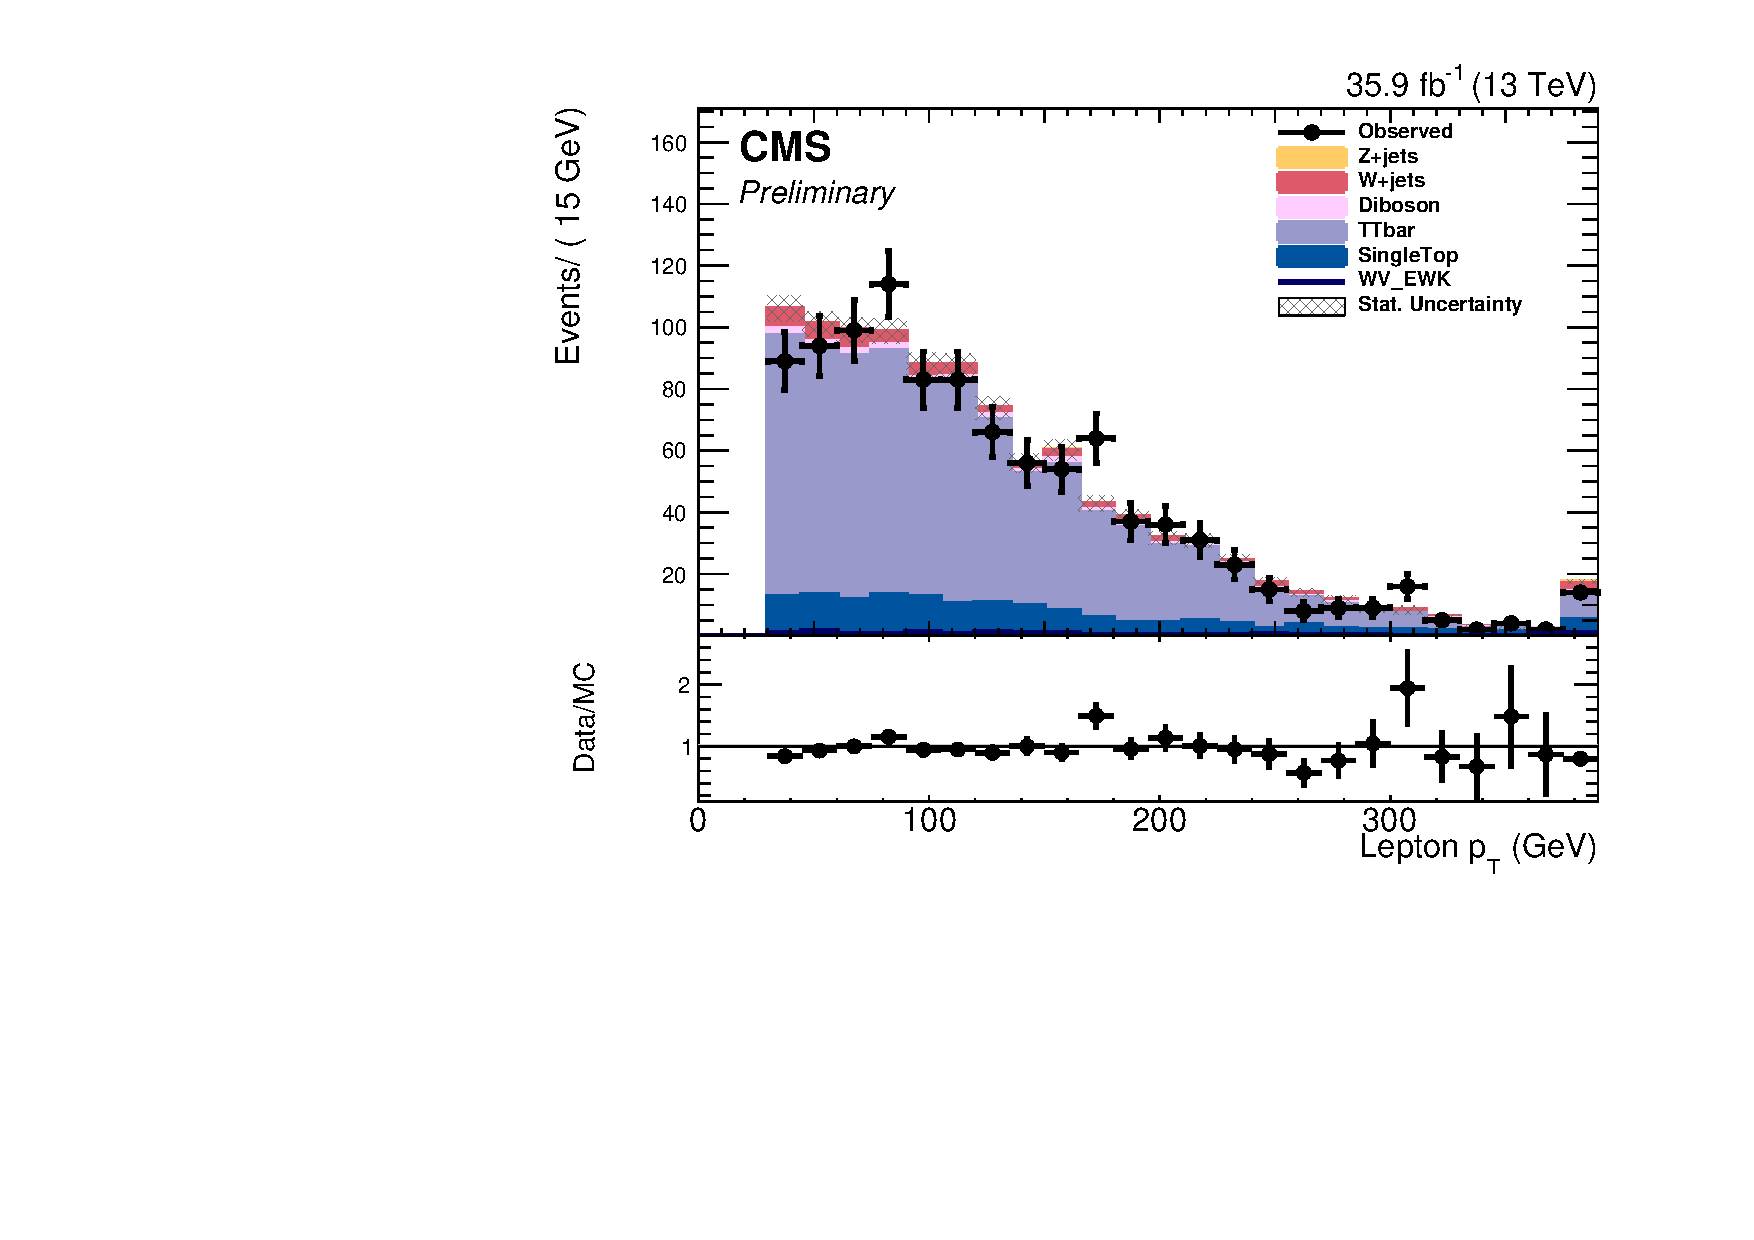
\includegraphics[width=0.45\textwidth]{Plots/plots/DibosonBoostedElMuCuts13TeV_TTBarControlRegion_CHS_lepton_pt.pdf}%
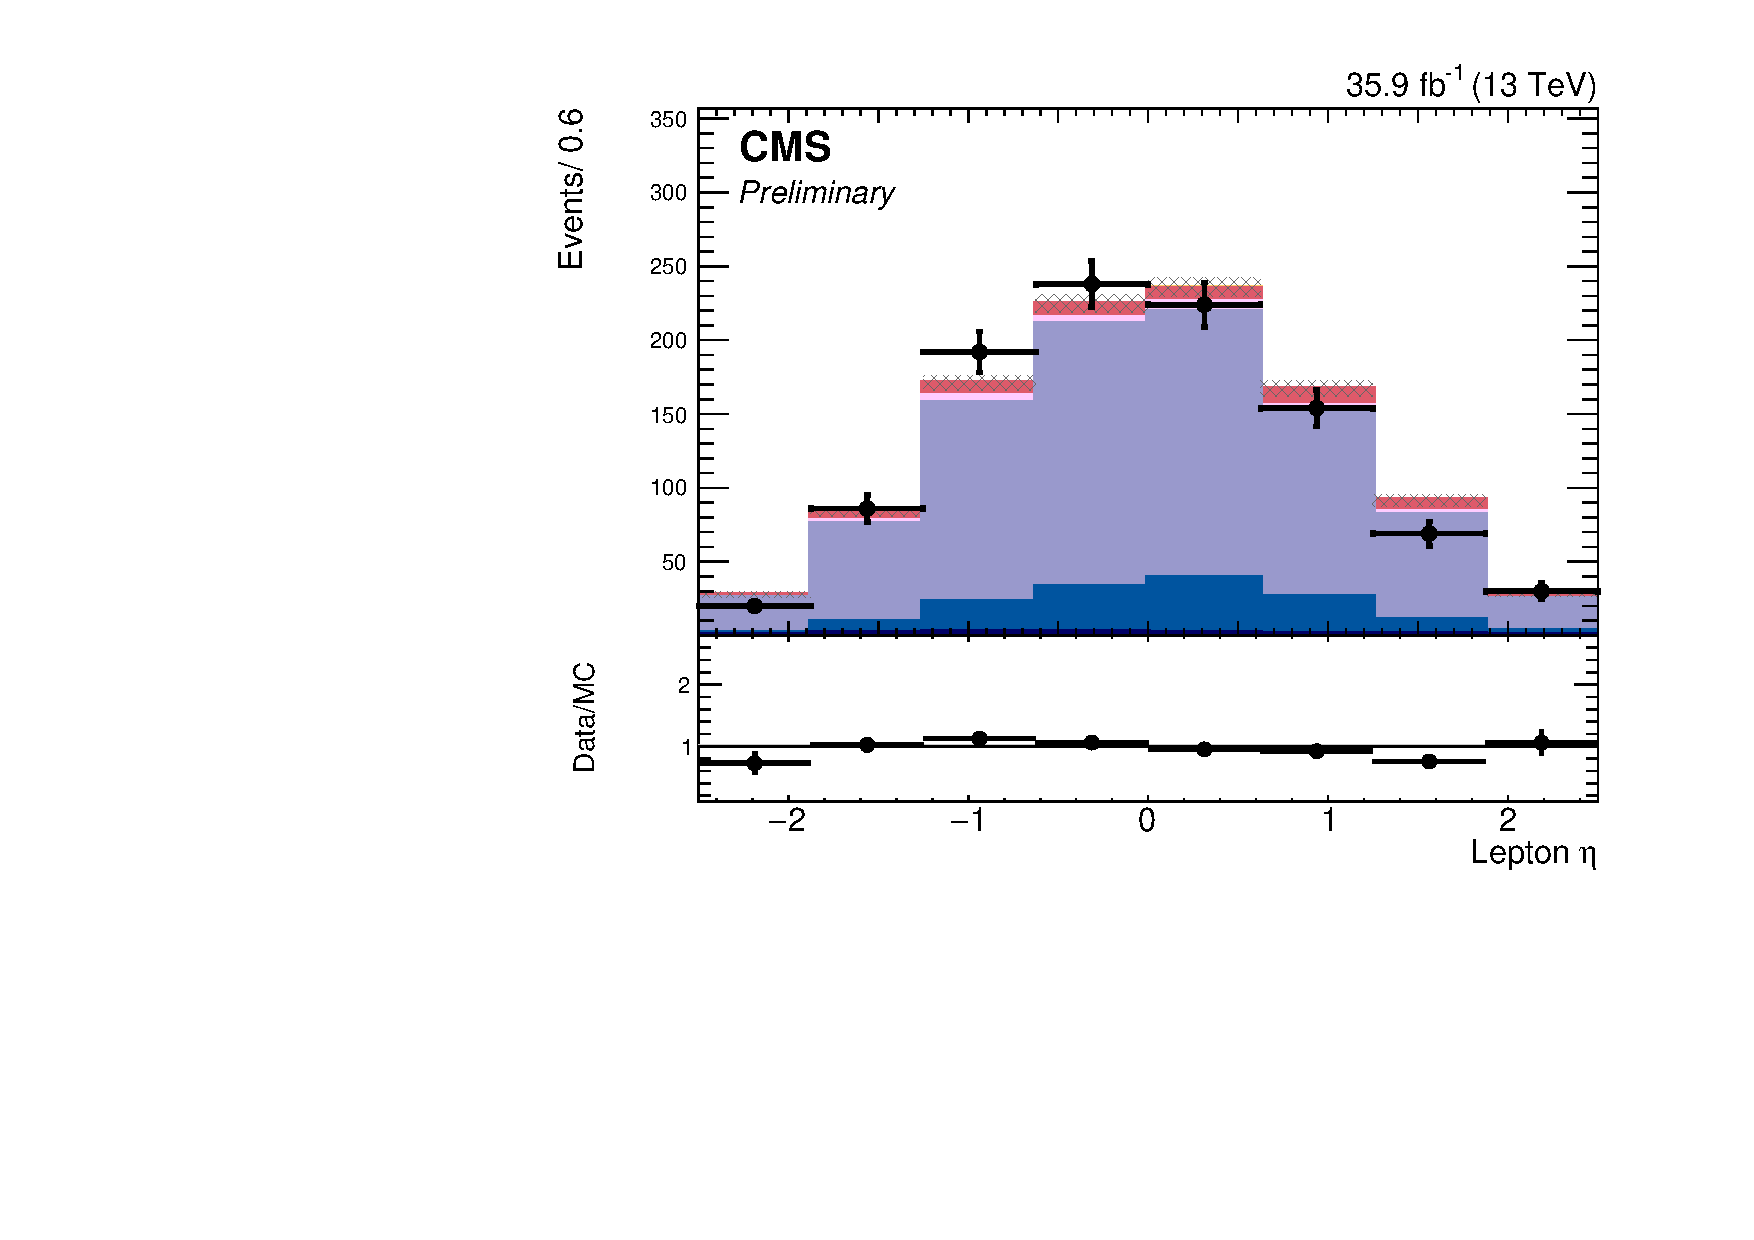
\includegraphics[width=0.45\textwidth]{Plots/plots/DibosonBoostedElMuCuts13TeV_TTBarControlRegion_CHS_lepton_eta.pdf}\\
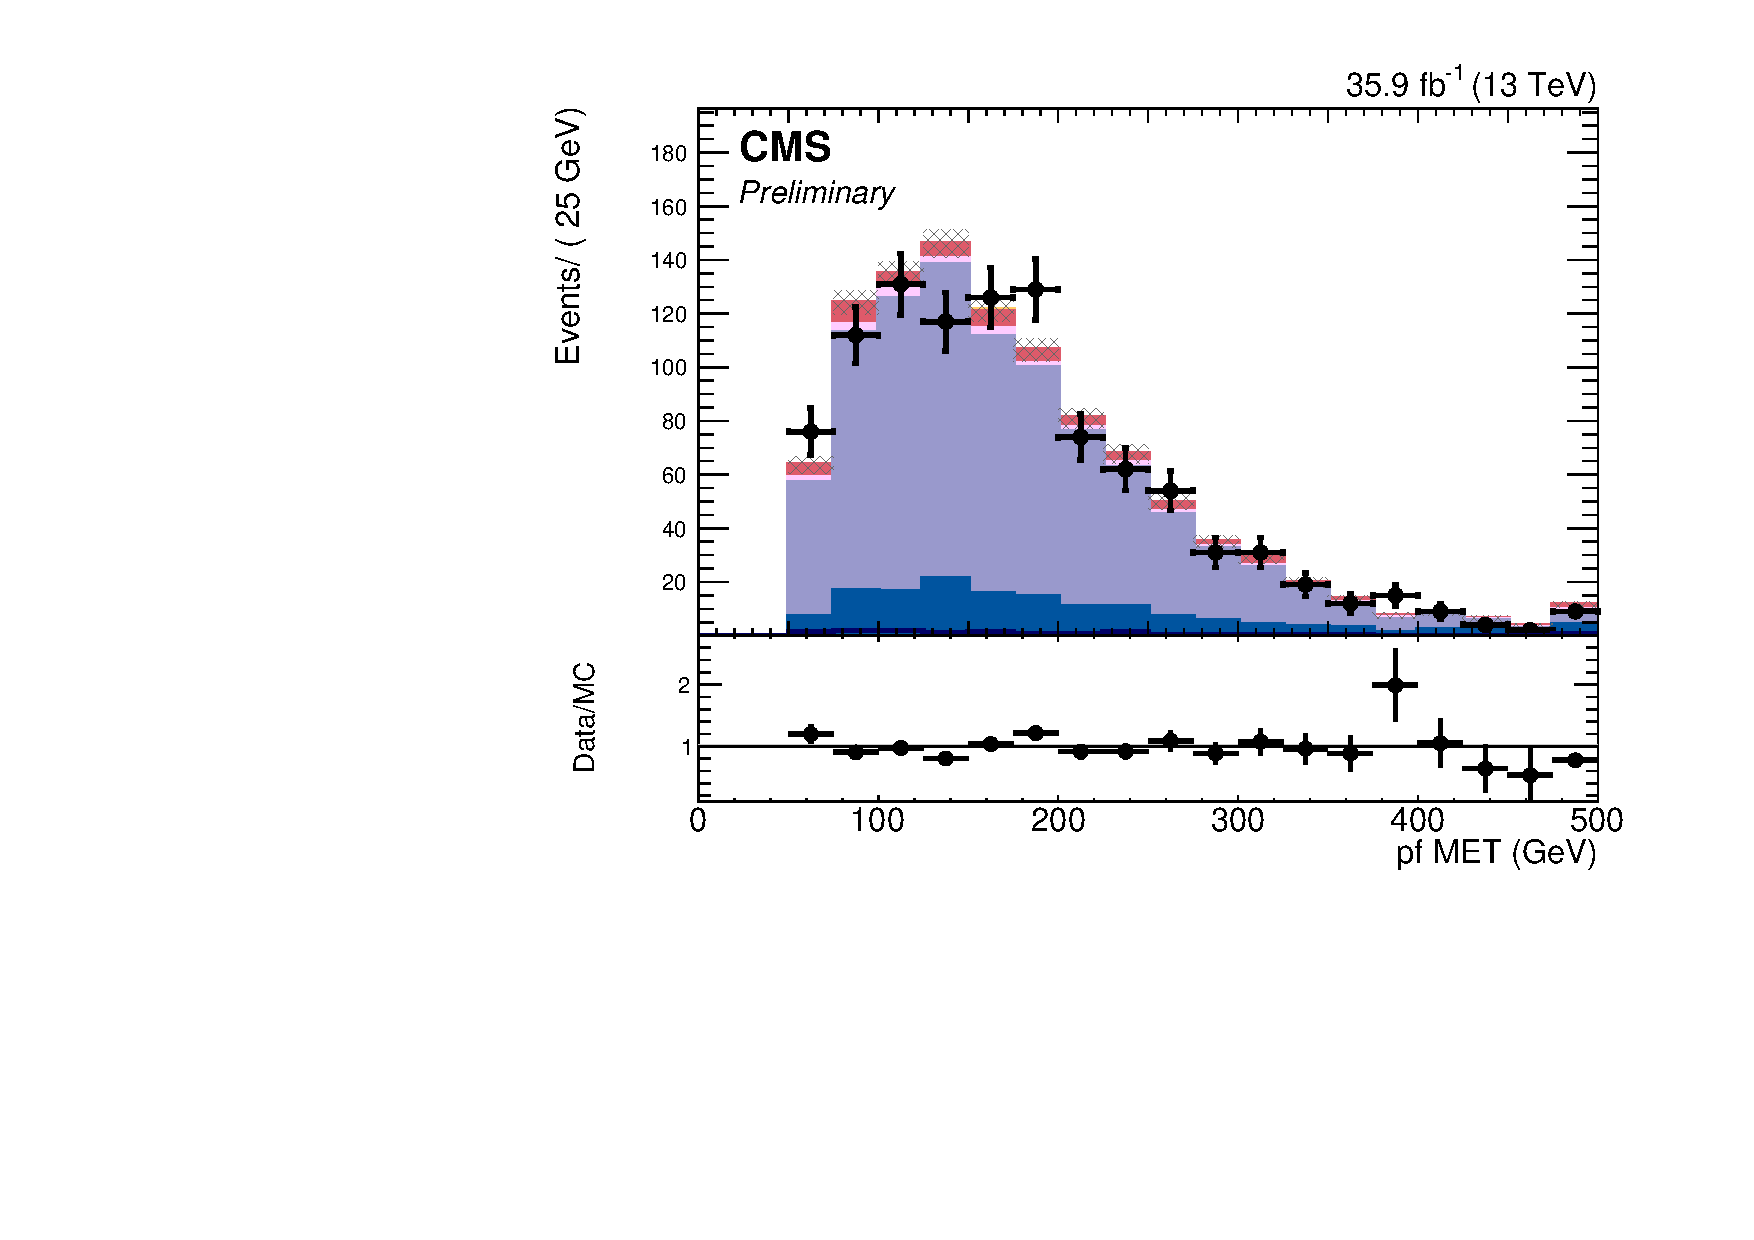
\includegraphics[width=0.45\textwidth]{Plots/plots/DibosonBoostedElMuCuts13TeV_TTBarControlRegion_CHS_pfMET_Corr.pdf}%
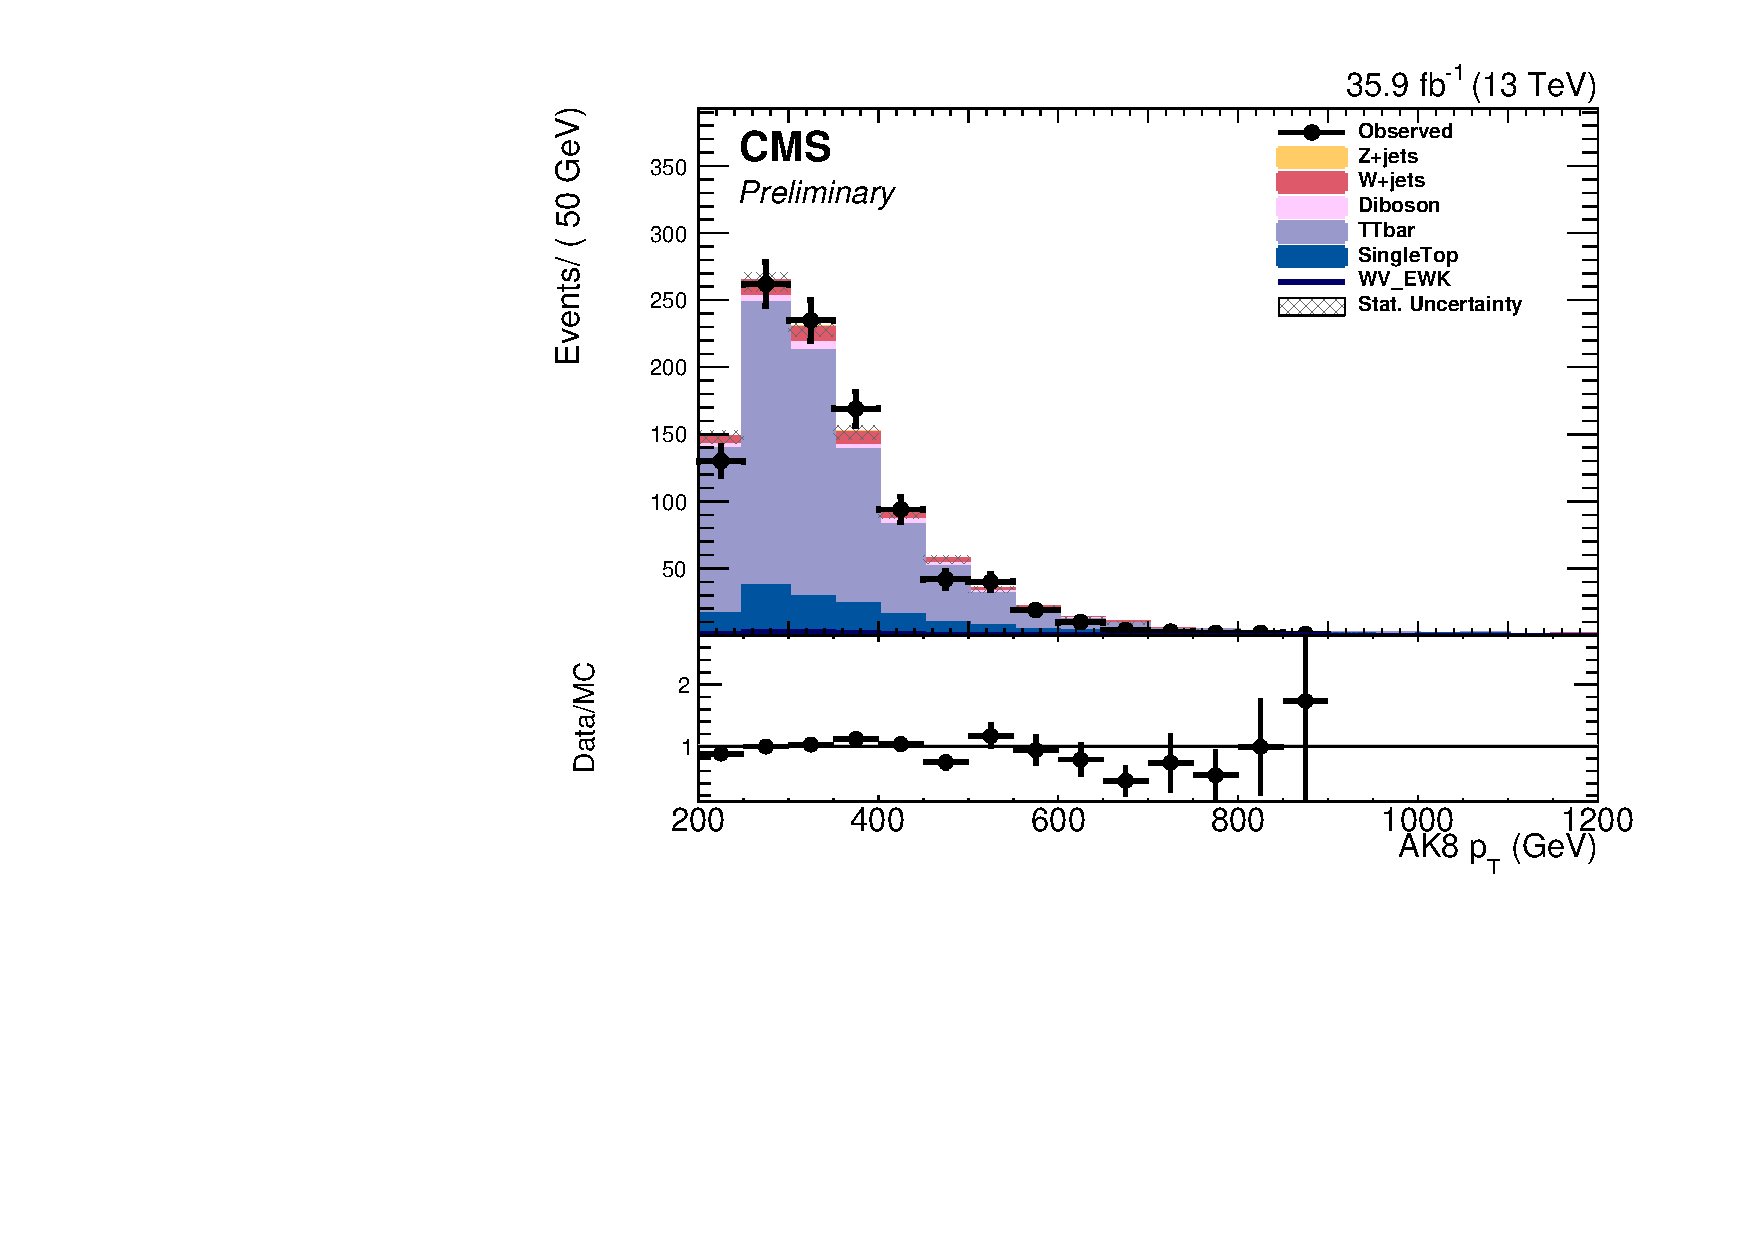
\includegraphics[width=0.45\textwidth]{Plots/plots/DibosonBoostedElMuCuts13TeV_TTBarControlRegion_CHS_ungroomed_PuppiAK8_jet_pt.pdf}\\
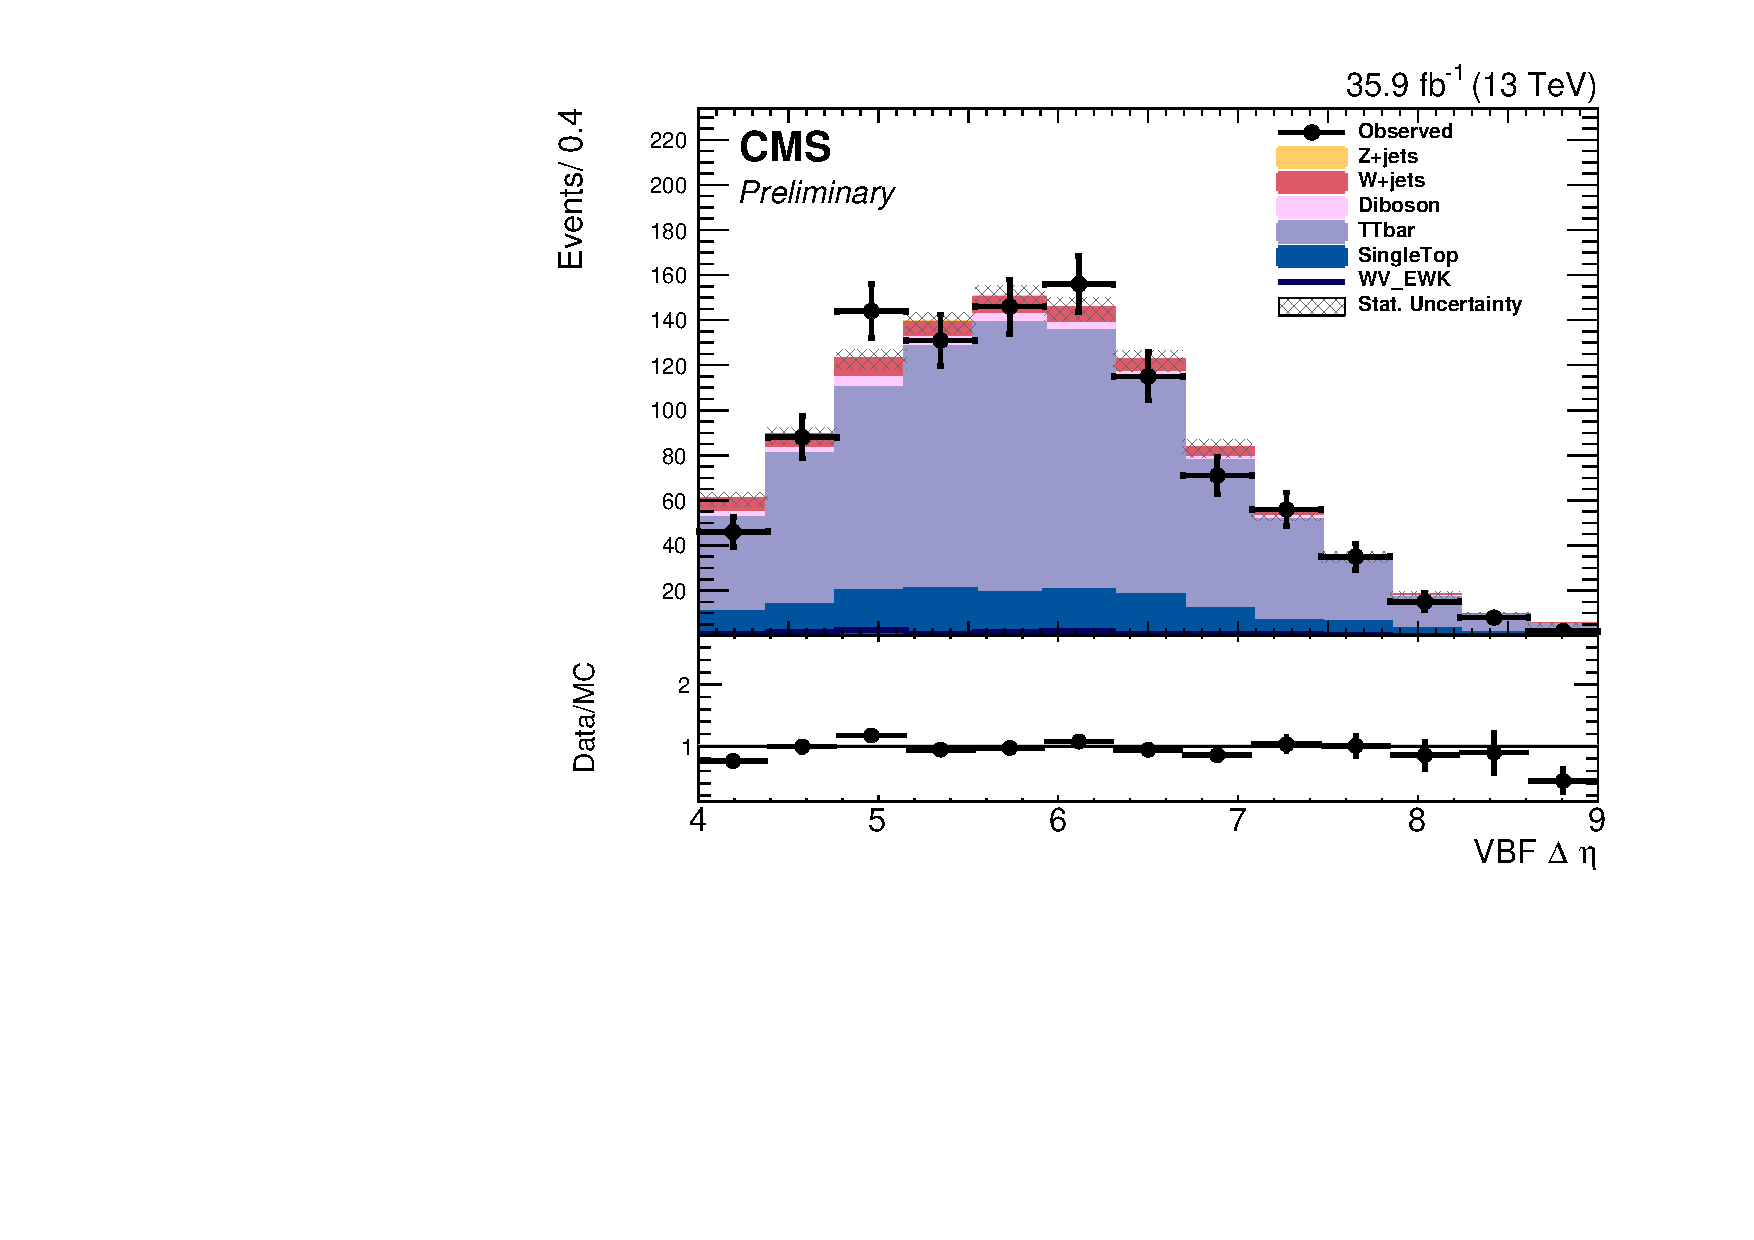
\includegraphics[width=0.45\textwidth]{Plots/plots/DibosonBoostedElMuCuts13TeV_TTBarControlRegion_CHS_vbf_maxpt_jj_Deta.pdf}%
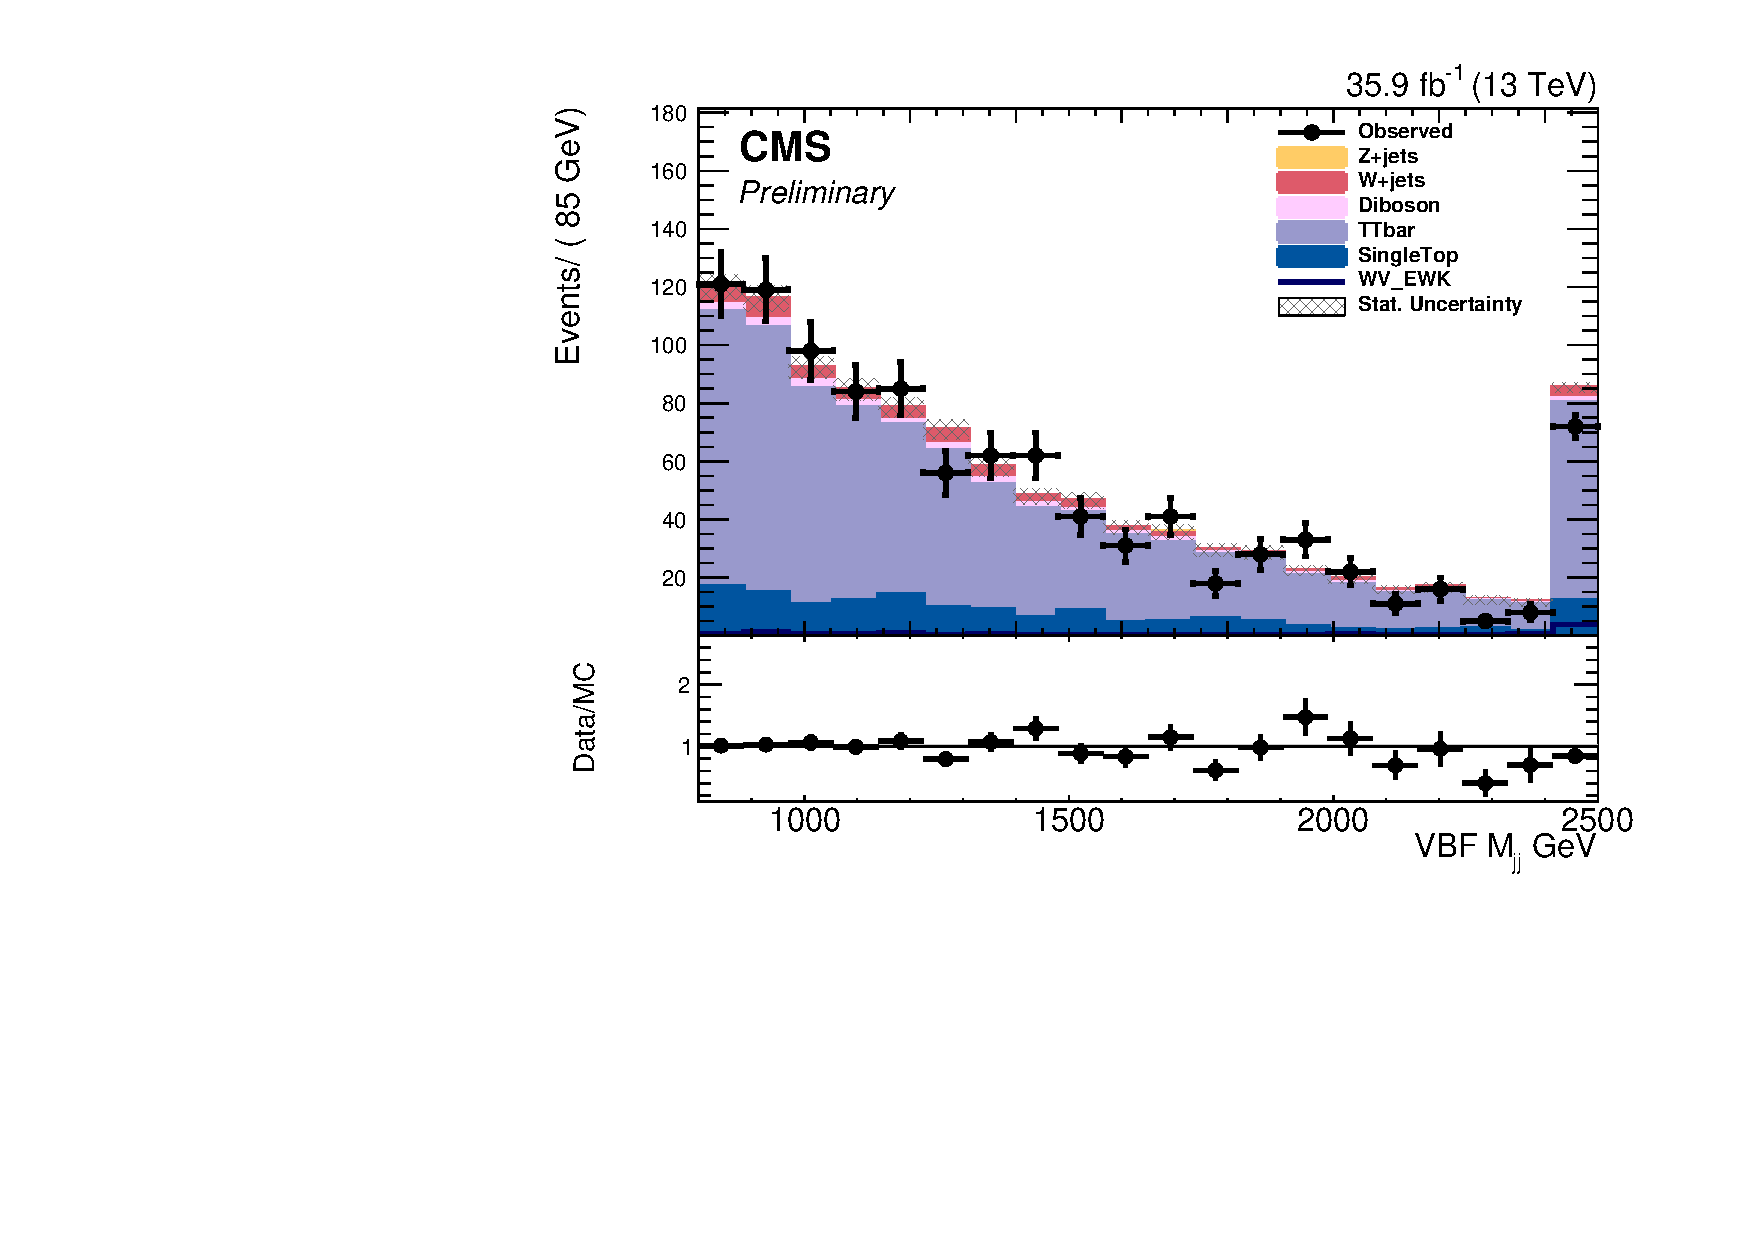
\includegraphics[width=0.45\textwidth]{Plots/plots/DibosonBoostedElMuCuts13TeV_TTBarControlRegion_CHS_vbf_maxpt_jj_m.pdf}\\
\caption{Kinematic distributions in the top background control region. The hatched bands include statistical uncertainties from the predicted yields.}
\label{fig:top_control}
\end{figure*}


\section{$W+$jets}
$W+$jets enriched control region is defined by selecting events with $40~GeV < m_{V} < 65~GeV$ or $105~GeV < m_{V} < 150~GeV$, where the full signal selection is applied. Figure~\ref{fig:wjet_control} shows the distributions of jet kinematic variables in this sideband region where $W+$jets predictions are taken from the simulation. Similarly, figure~\ref{fig:wjet_control2} shows the distributions of the lepton, $\ptmiss$, and $V$ jet kinematic distributions. 

\begin{figure*}[htb]
\centering
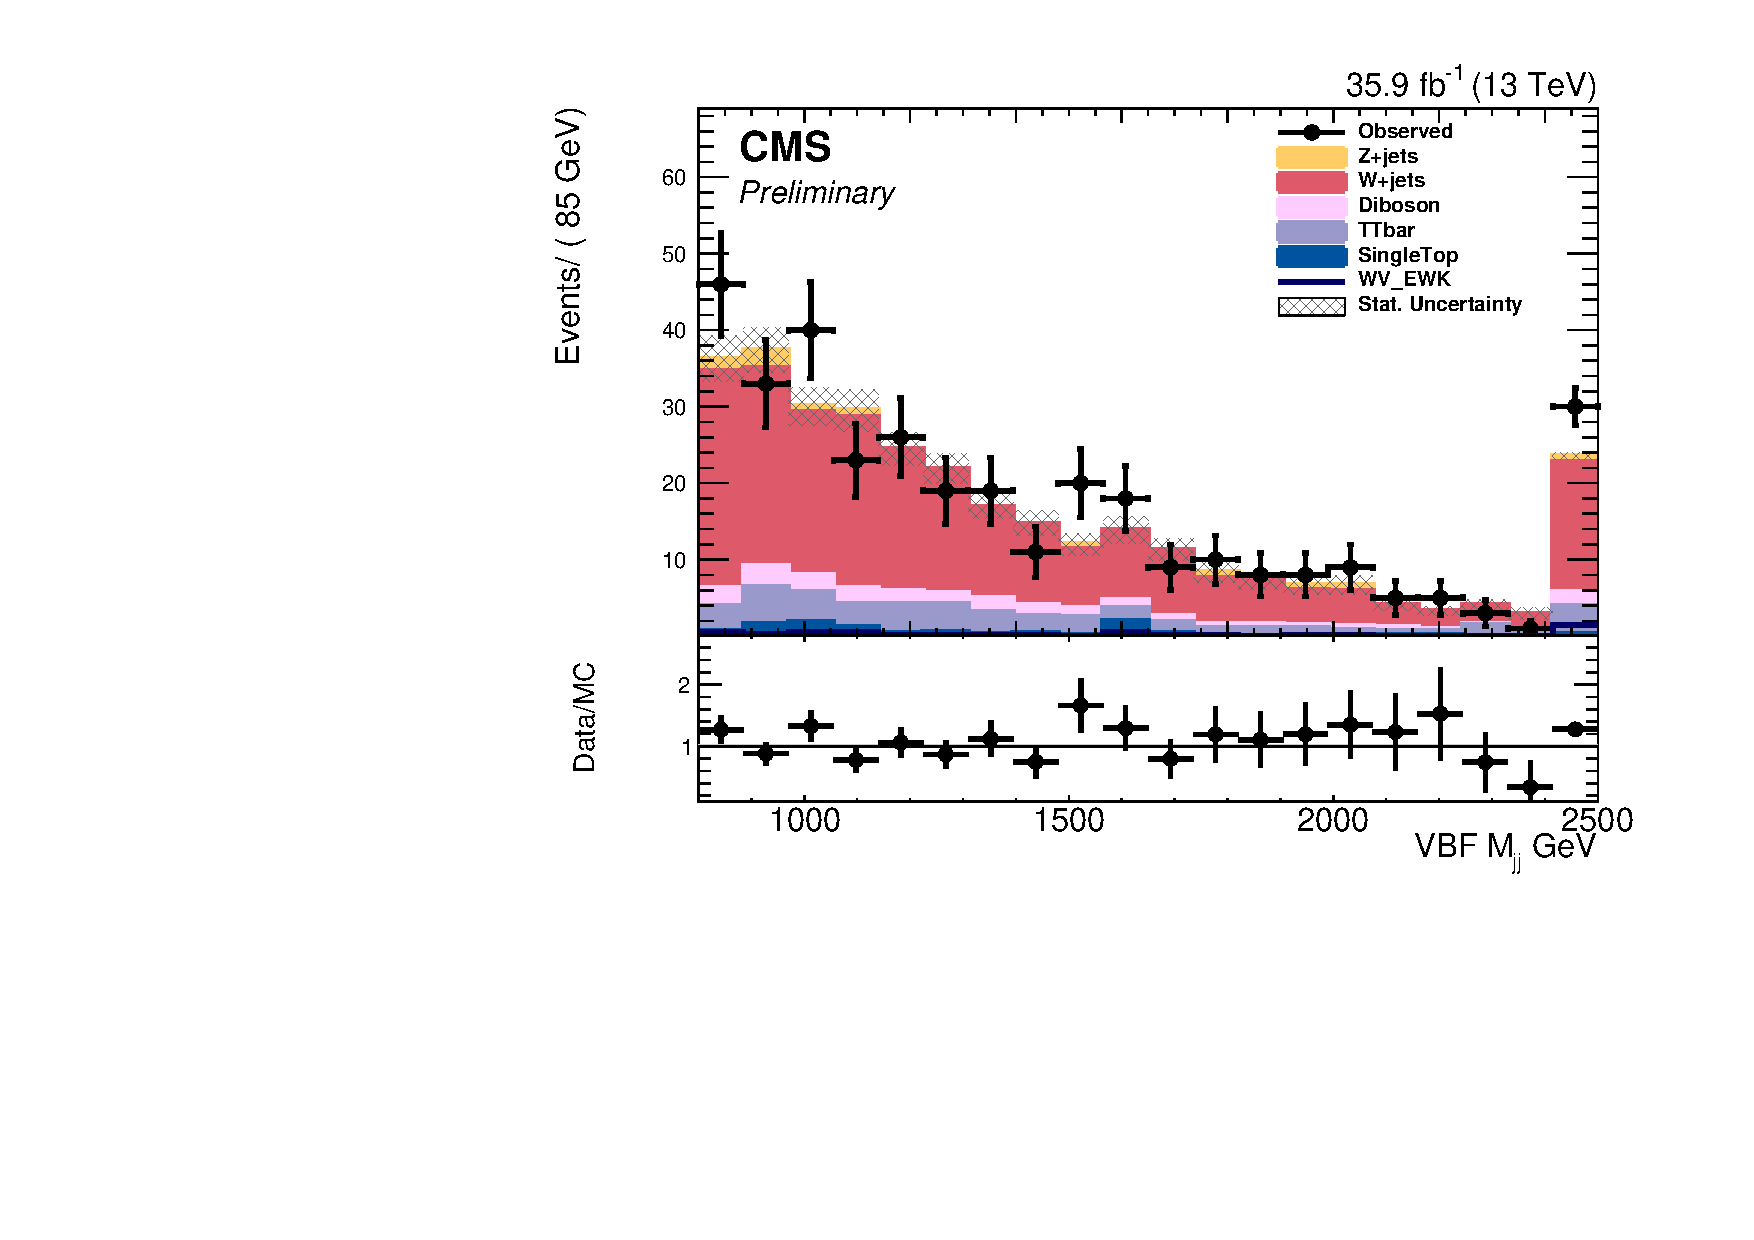
\includegraphics[width=0.45\textwidth]{Plots/plots/DibosonBoostedElMuCuts13TeV_WjetControlRegion_Tighter_CHS_vbf_maxpt_jj_m.pdf}%
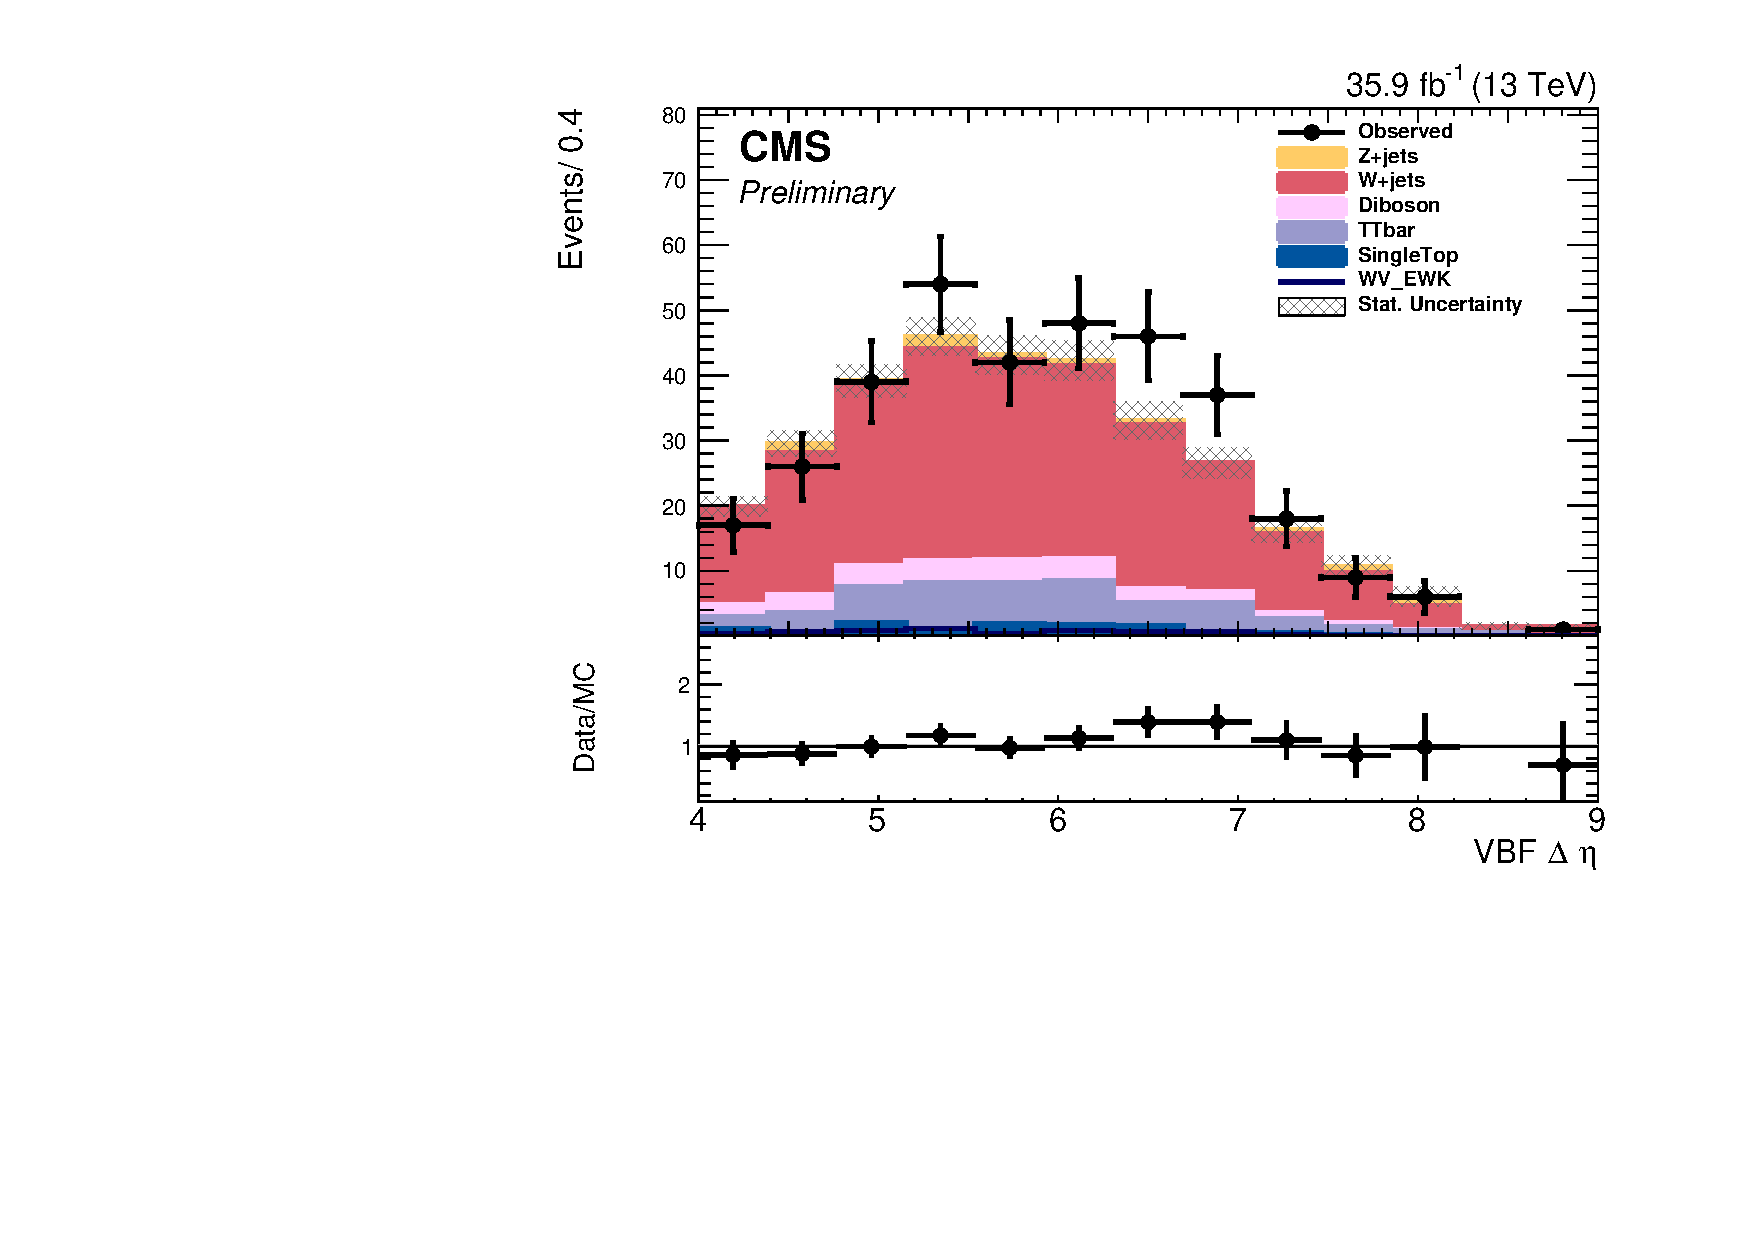
\includegraphics[width=0.45\textwidth]{Plots/plots/DibosonBoostedElMuCuts13TeV_WjetControlRegion_Tighter_CHS_vbf_maxpt_jj_Deta.pdf}\\
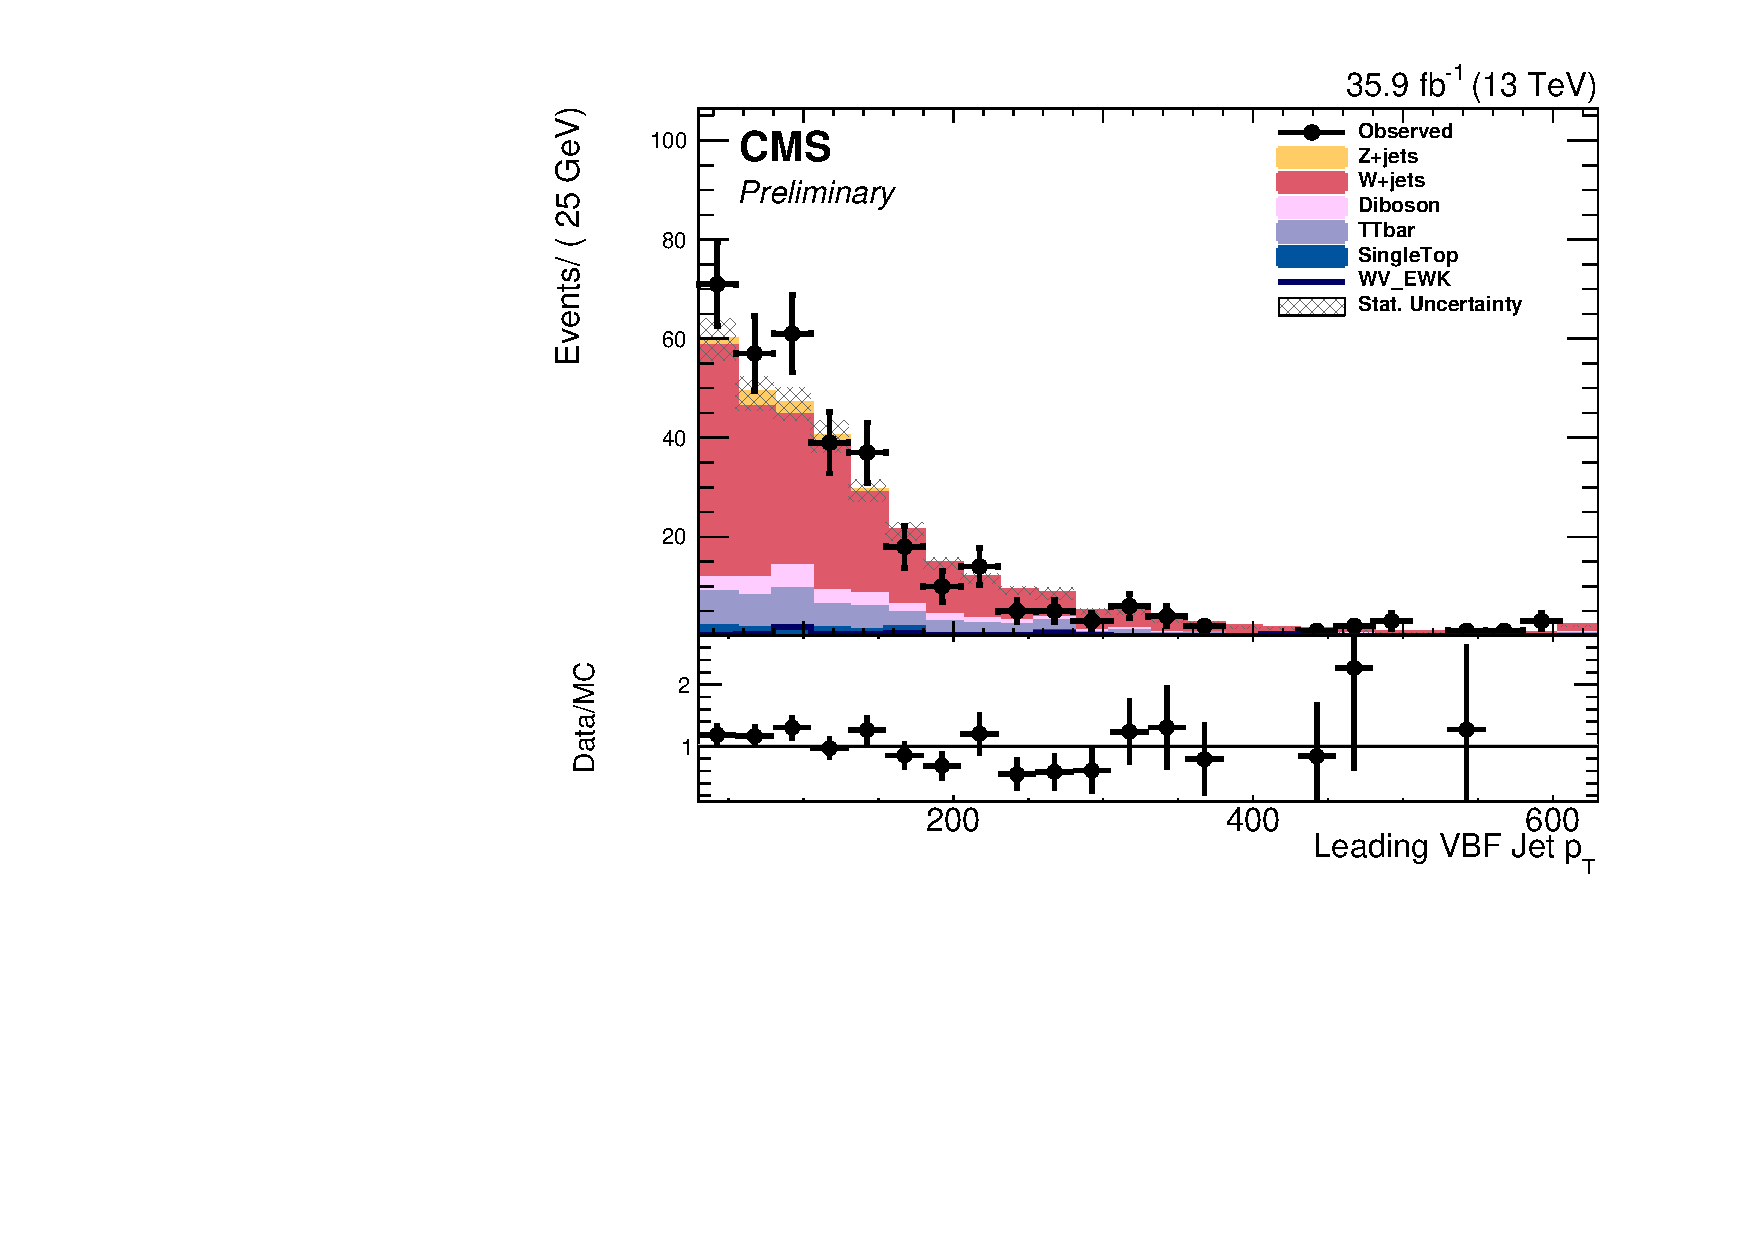
\includegraphics[width=0.45\textwidth]{Plots/plots/DibosonBoostedElMuCuts13TeV_WjetControlRegion_Tighter_CHS_vbf_maxpt_j1_pt.pdf}%
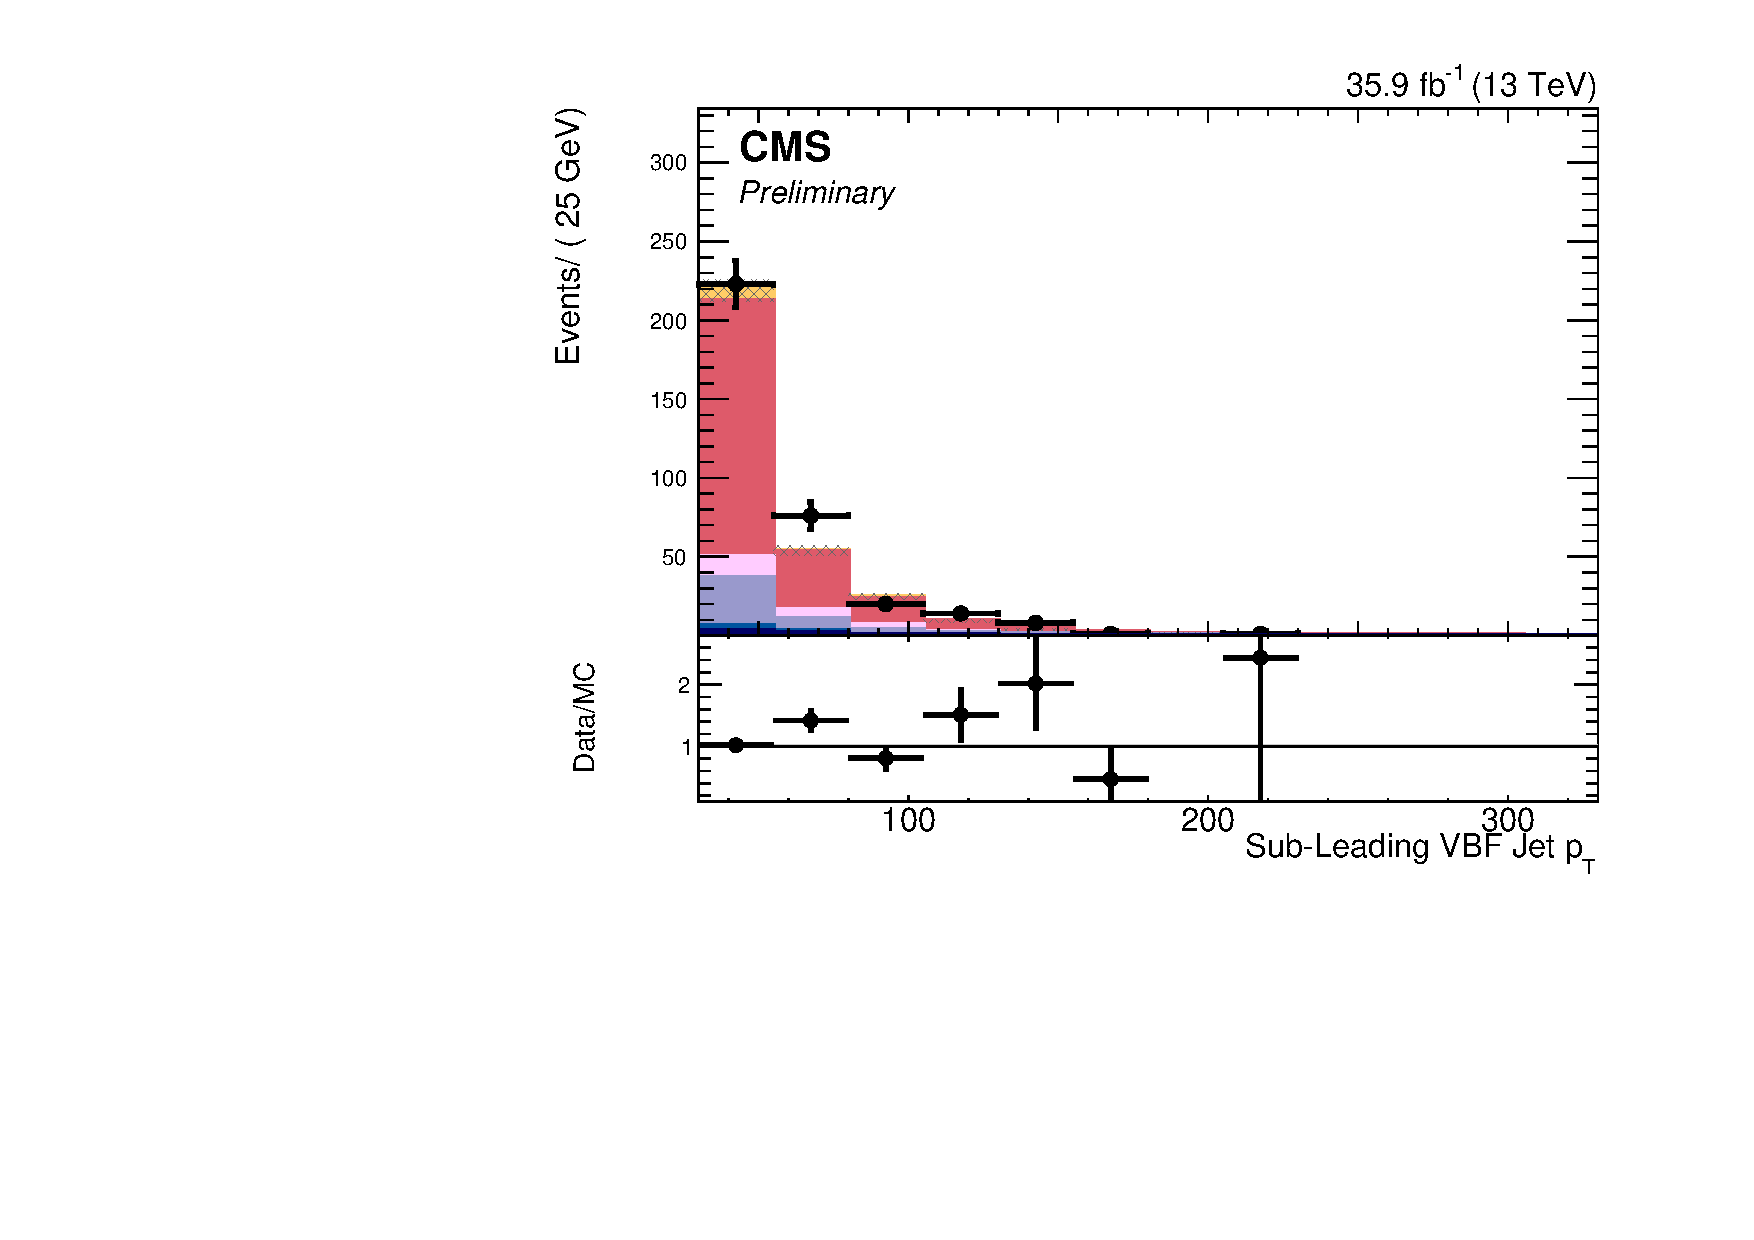
\includegraphics[width=0.45\textwidth]{Plots/plots/DibosonBoostedElMuCuts13TeV_WjetControlRegion_Tighter_CHS_vbf_maxpt_j2_pt.pdf}\\
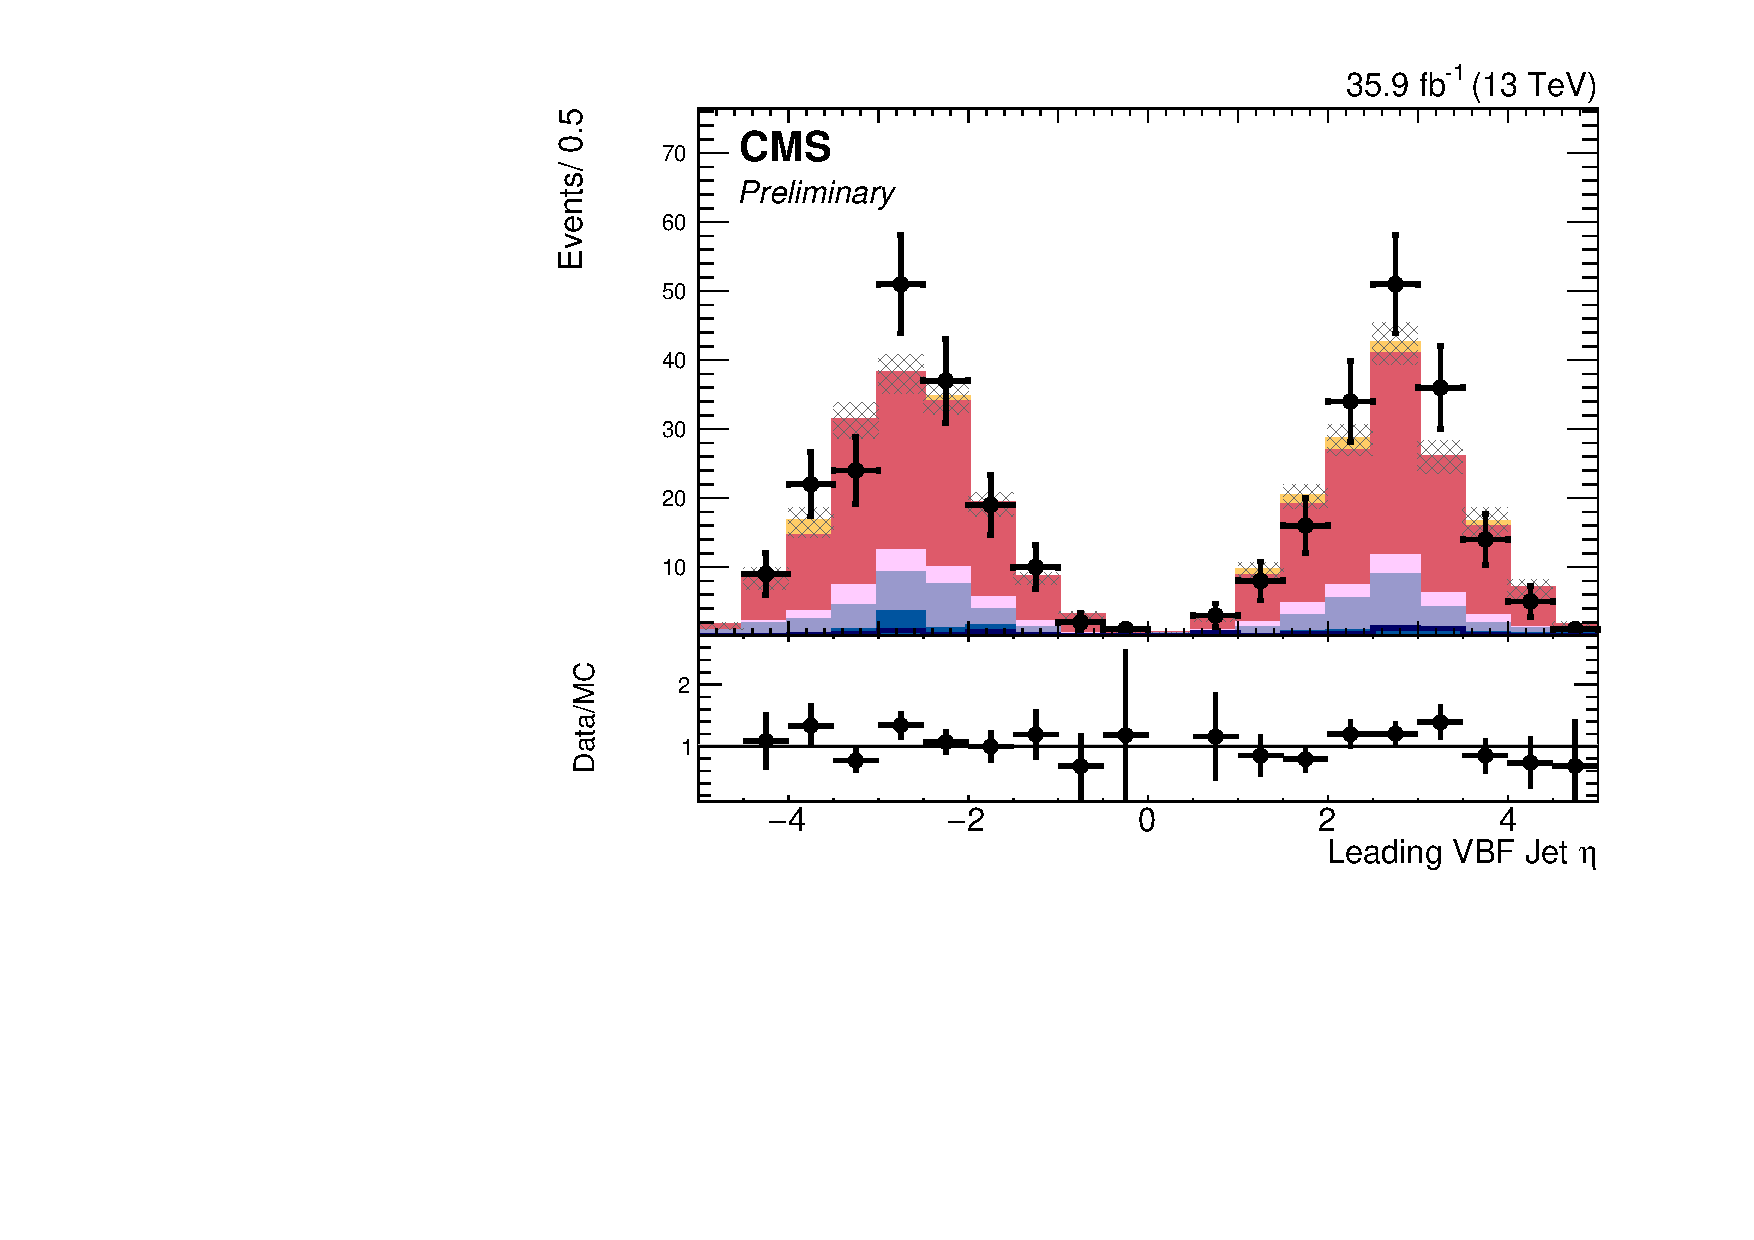
\includegraphics[width=0.45\textwidth]{Plots/plots/DibosonBoostedElMuCuts13TeV_WjetControlRegion_Tighter_CHS_vbf_maxpt_j1_eta.pdf}%
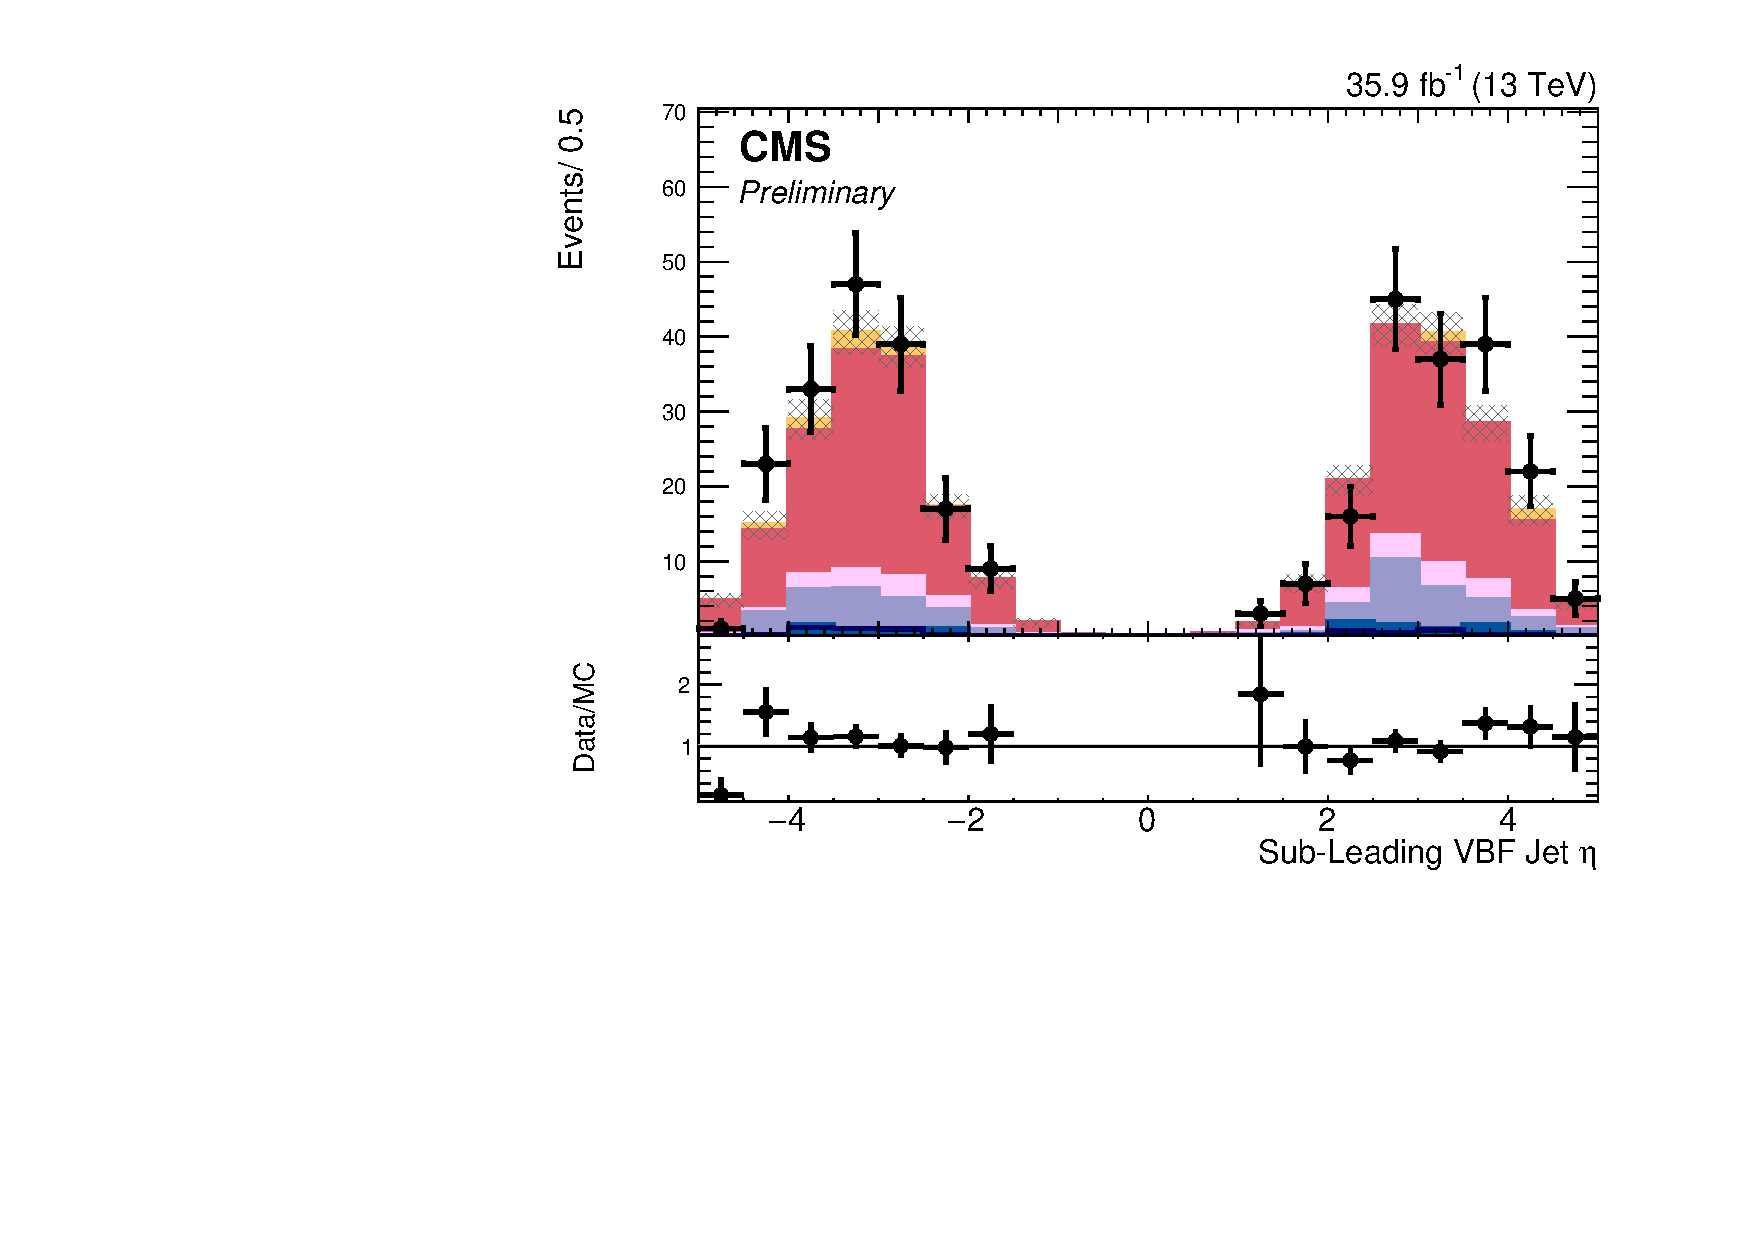
\includegraphics[width=0.45\textwidth]{Plots/plots/DibosonBoostedElMuCuts13TeV_WjetControlRegion_Tighter_CHS_vbf_maxpt_j2_eta.pdf}\\
\caption{Kinematic distributions in the $W+$jets background sideband region. $W+$jets predictions are taken from the simulation. The hatched bands include statistical uncertainties from the predicted yields.}
\label{fig:wjet_control}
\end{figure*}
 
\begin{figure*}[htb]
\centering
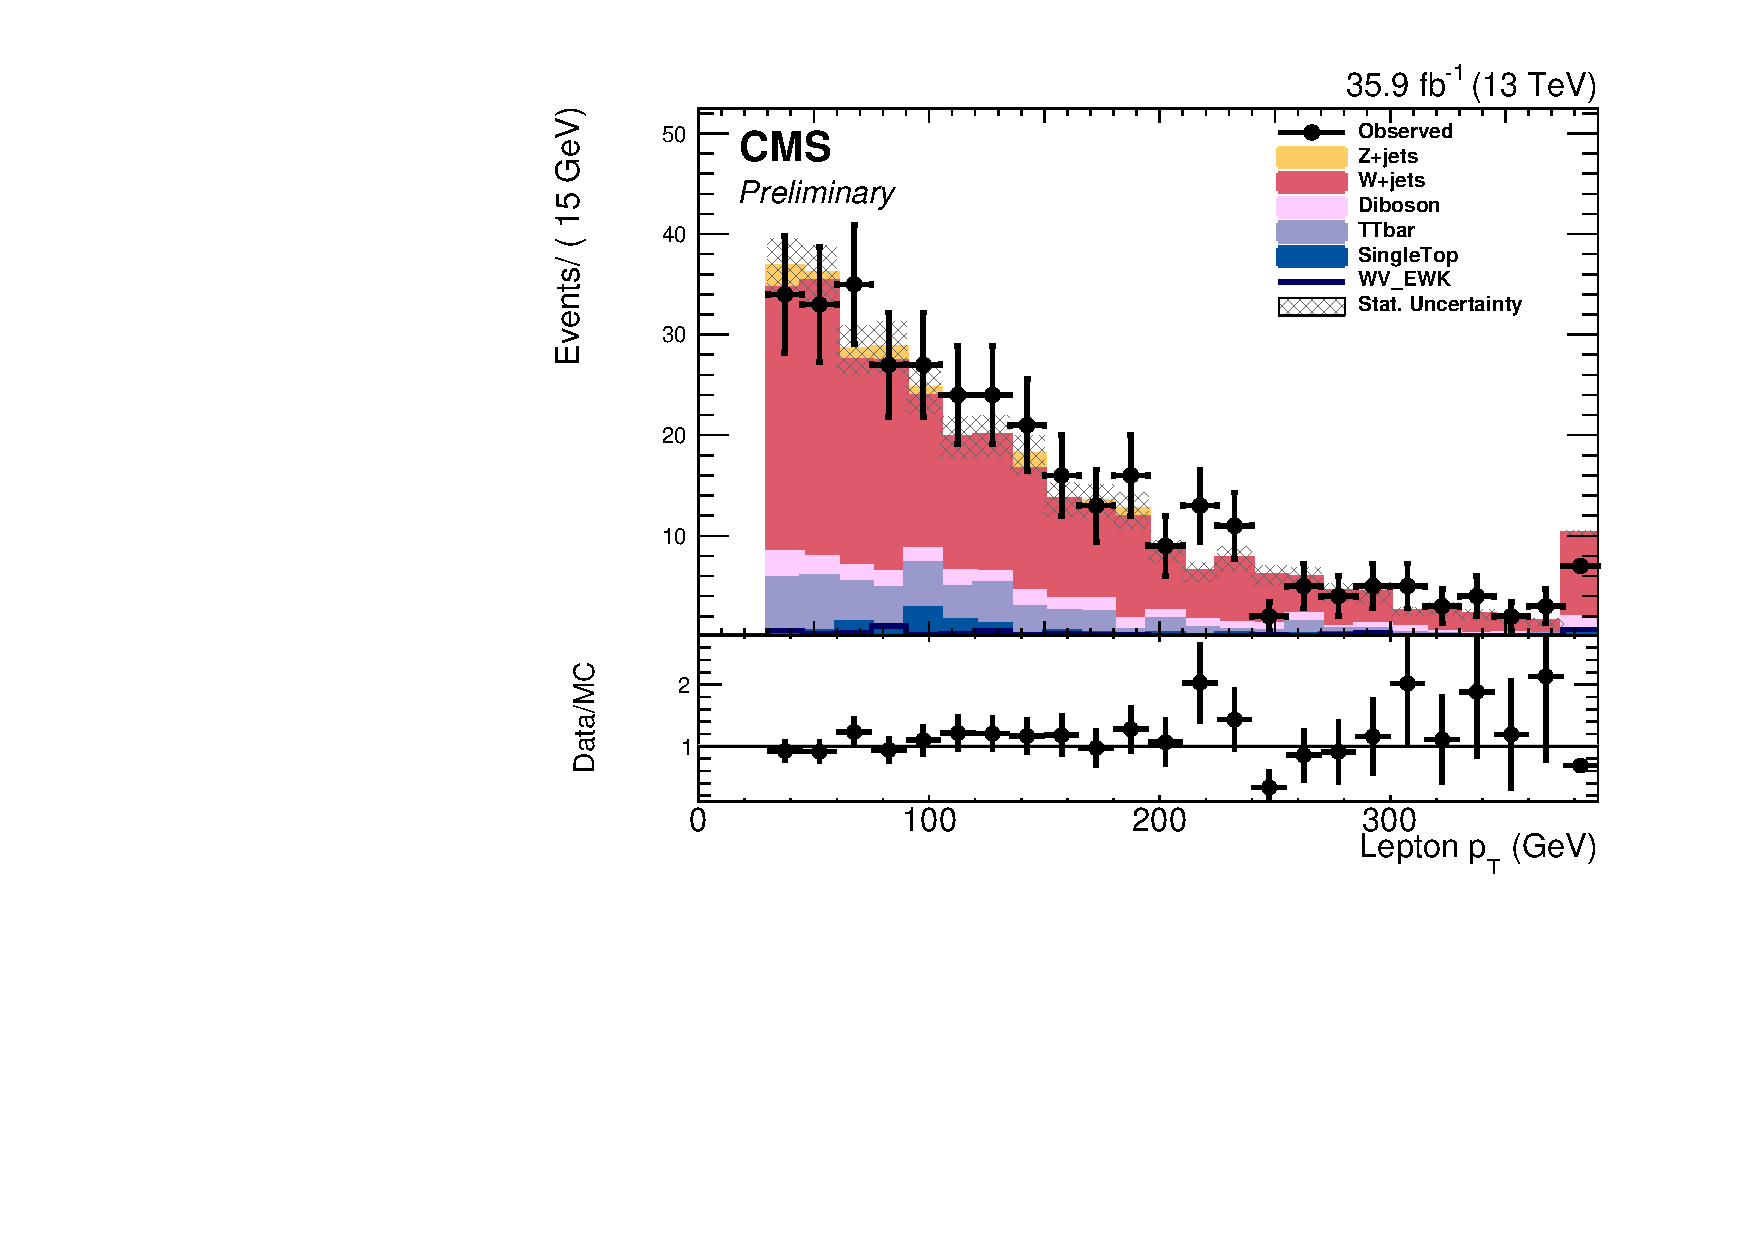
\includegraphics[width=0.45\textwidth]{Plots/plots/DibosonBoostedElMuCuts13TeV_WjetControlRegion_Tighter_CHS_lepton_pt.pdf}%
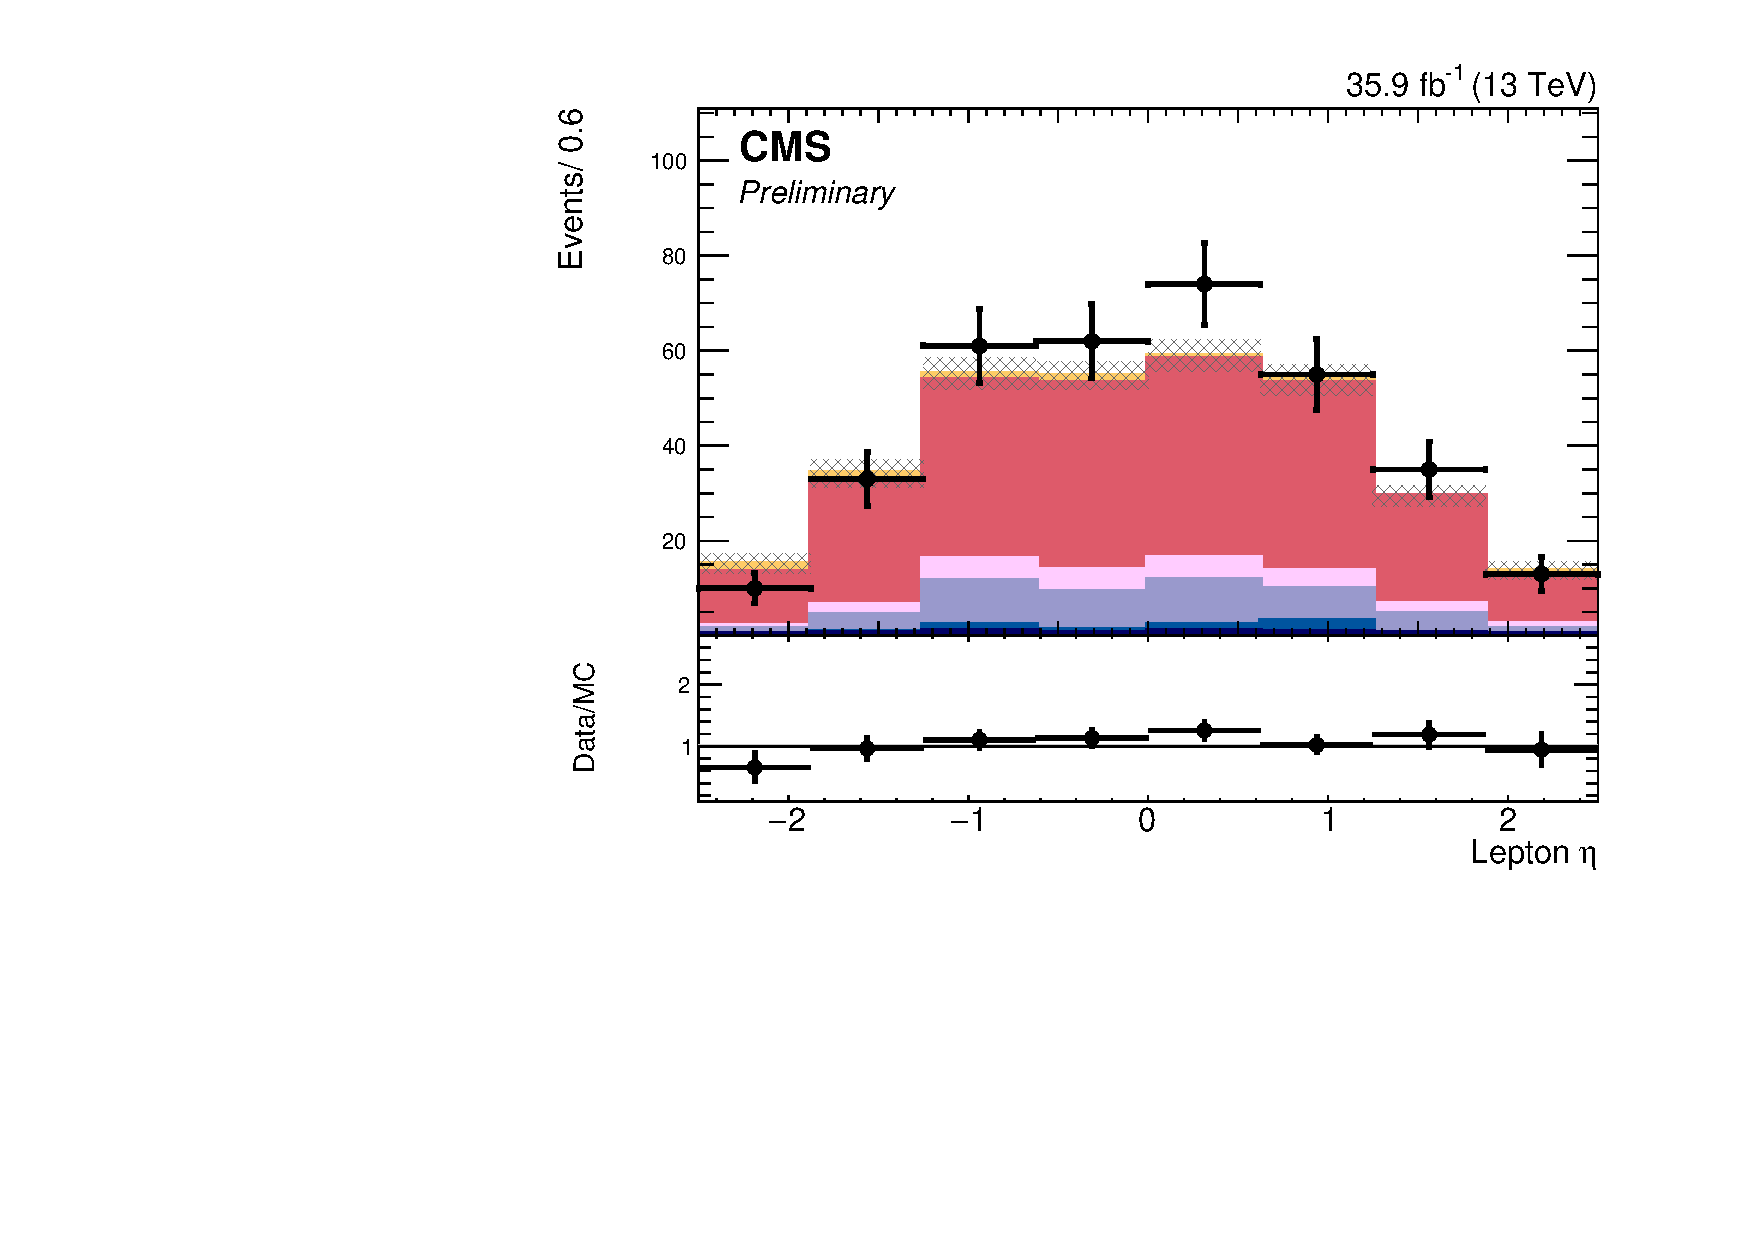
\includegraphics[width=0.45\textwidth]{Plots/plots/DibosonBoostedElMuCuts13TeV_WjetControlRegion_Tighter_CHS_lepton_eta.pdf}\\
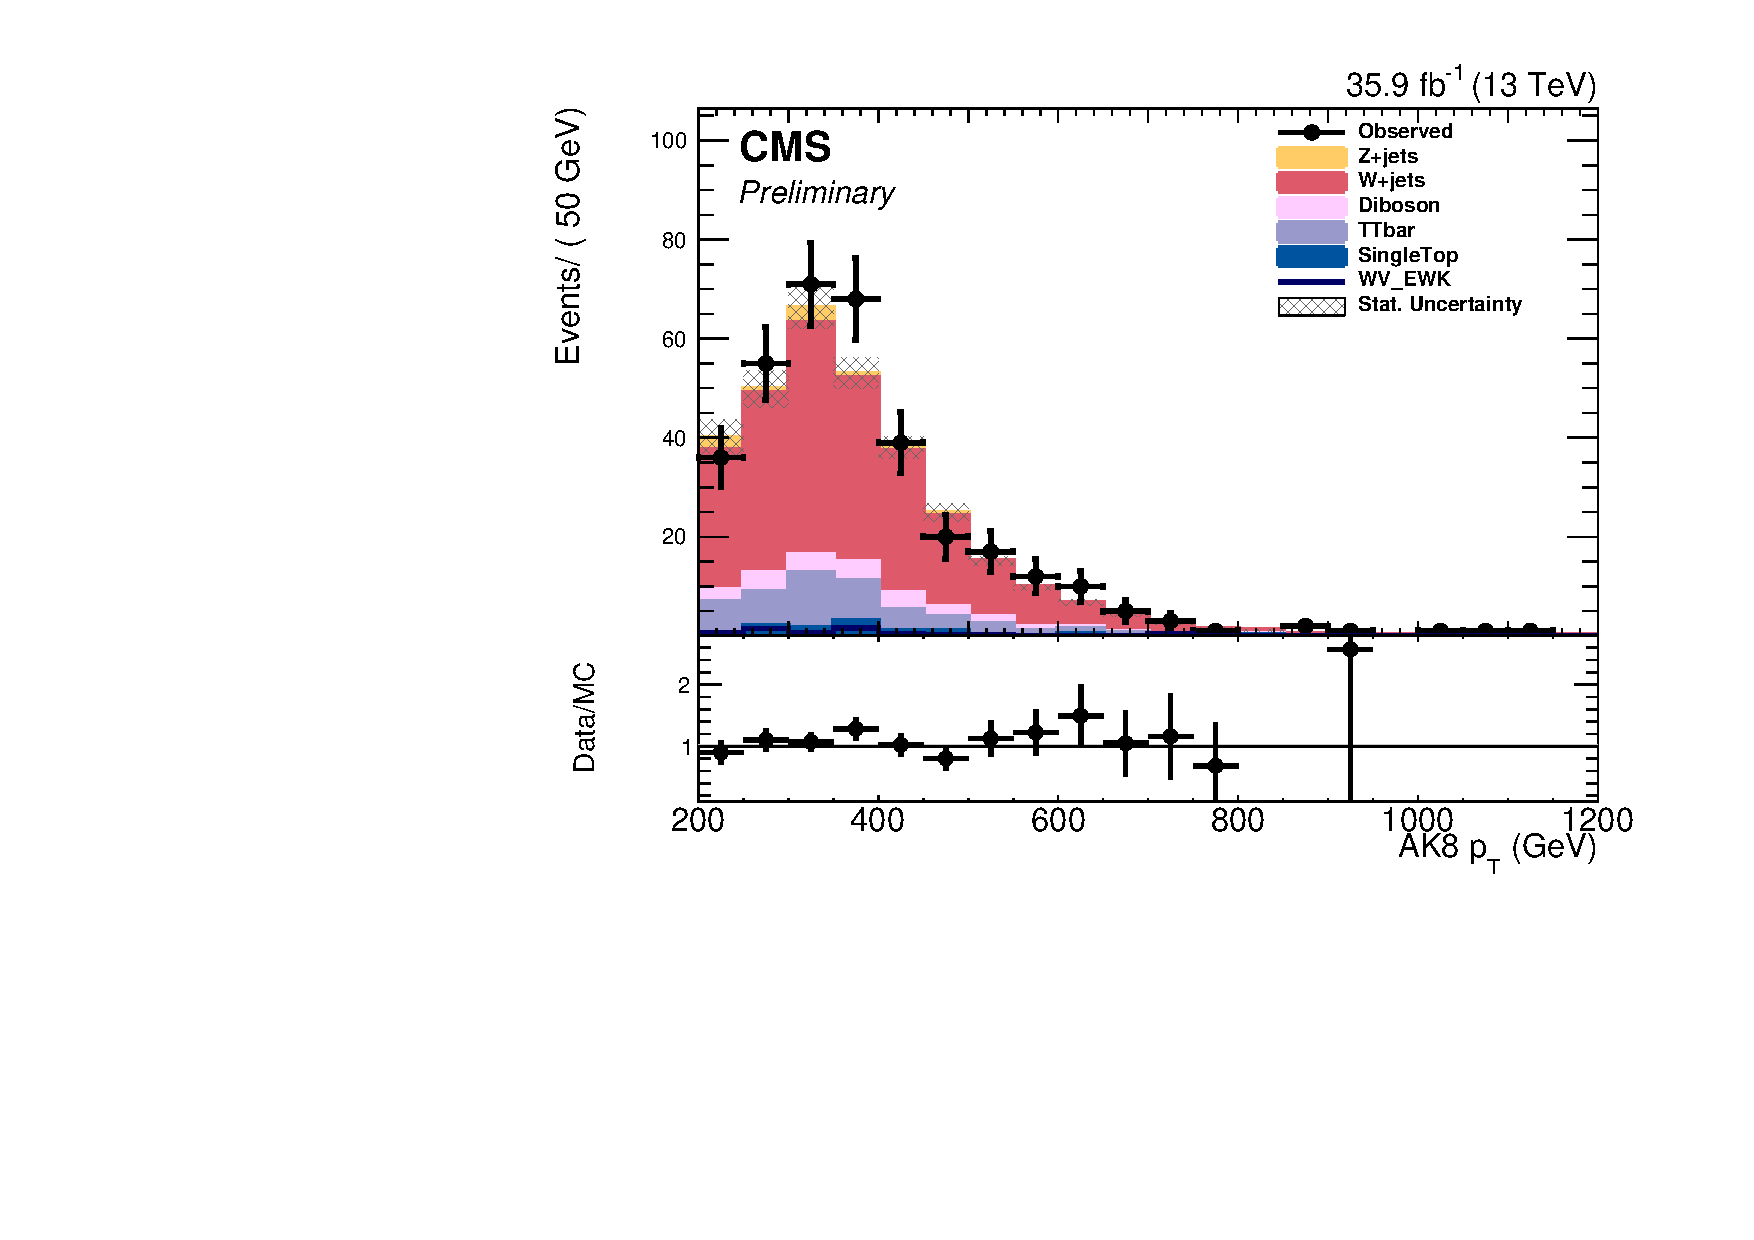
\includegraphics[width=0.45\textwidth]{Plots/plots/DibosonBoostedElMuCuts13TeV_WjetControlRegion_Tighter_CHS_ungroomed_PuppiAK8_jet_pt.pdf}%
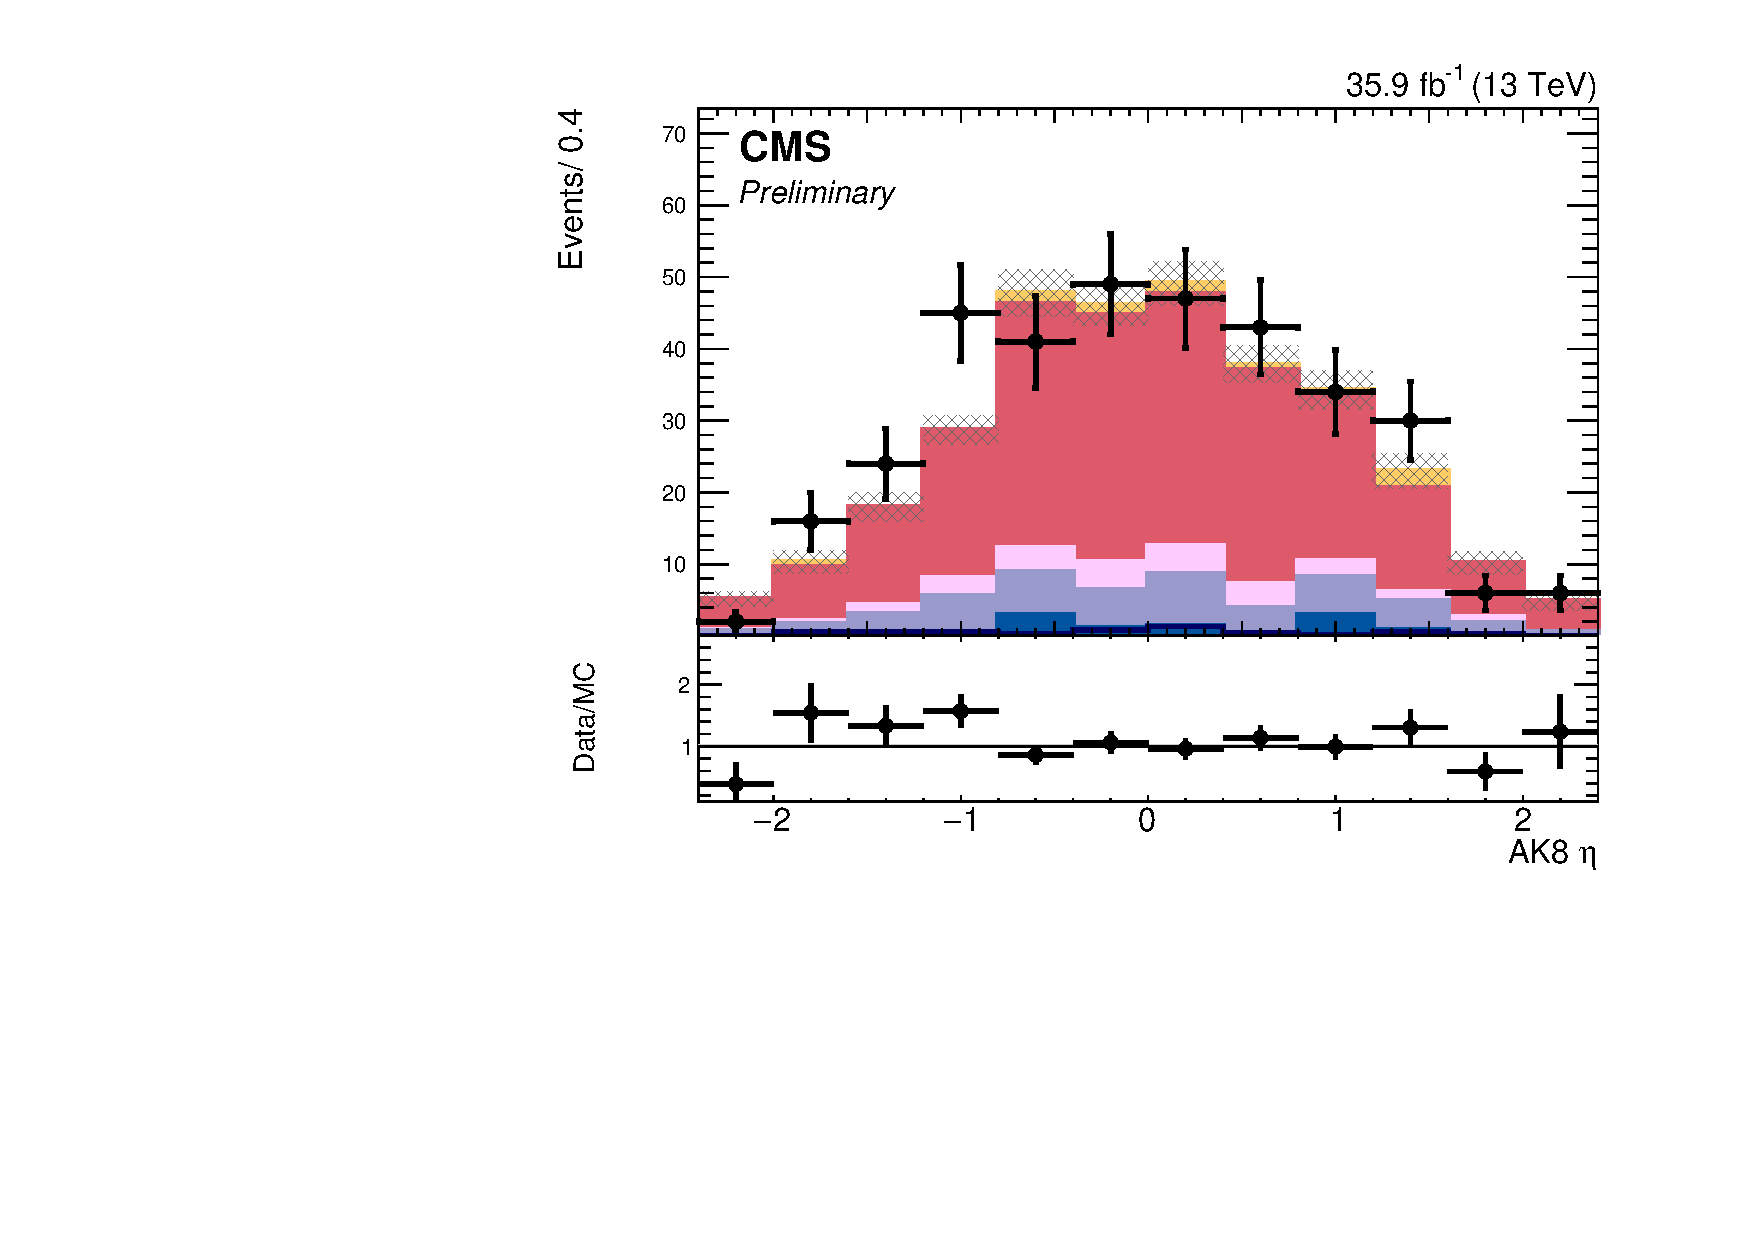
\includegraphics[width=0.45\textwidth]{Plots/plots/DibosonBoostedElMuCuts13TeV_WjetControlRegion_Tighter_CHS_ungroomed_PuppiAK8_jet_eta.pdf}\\
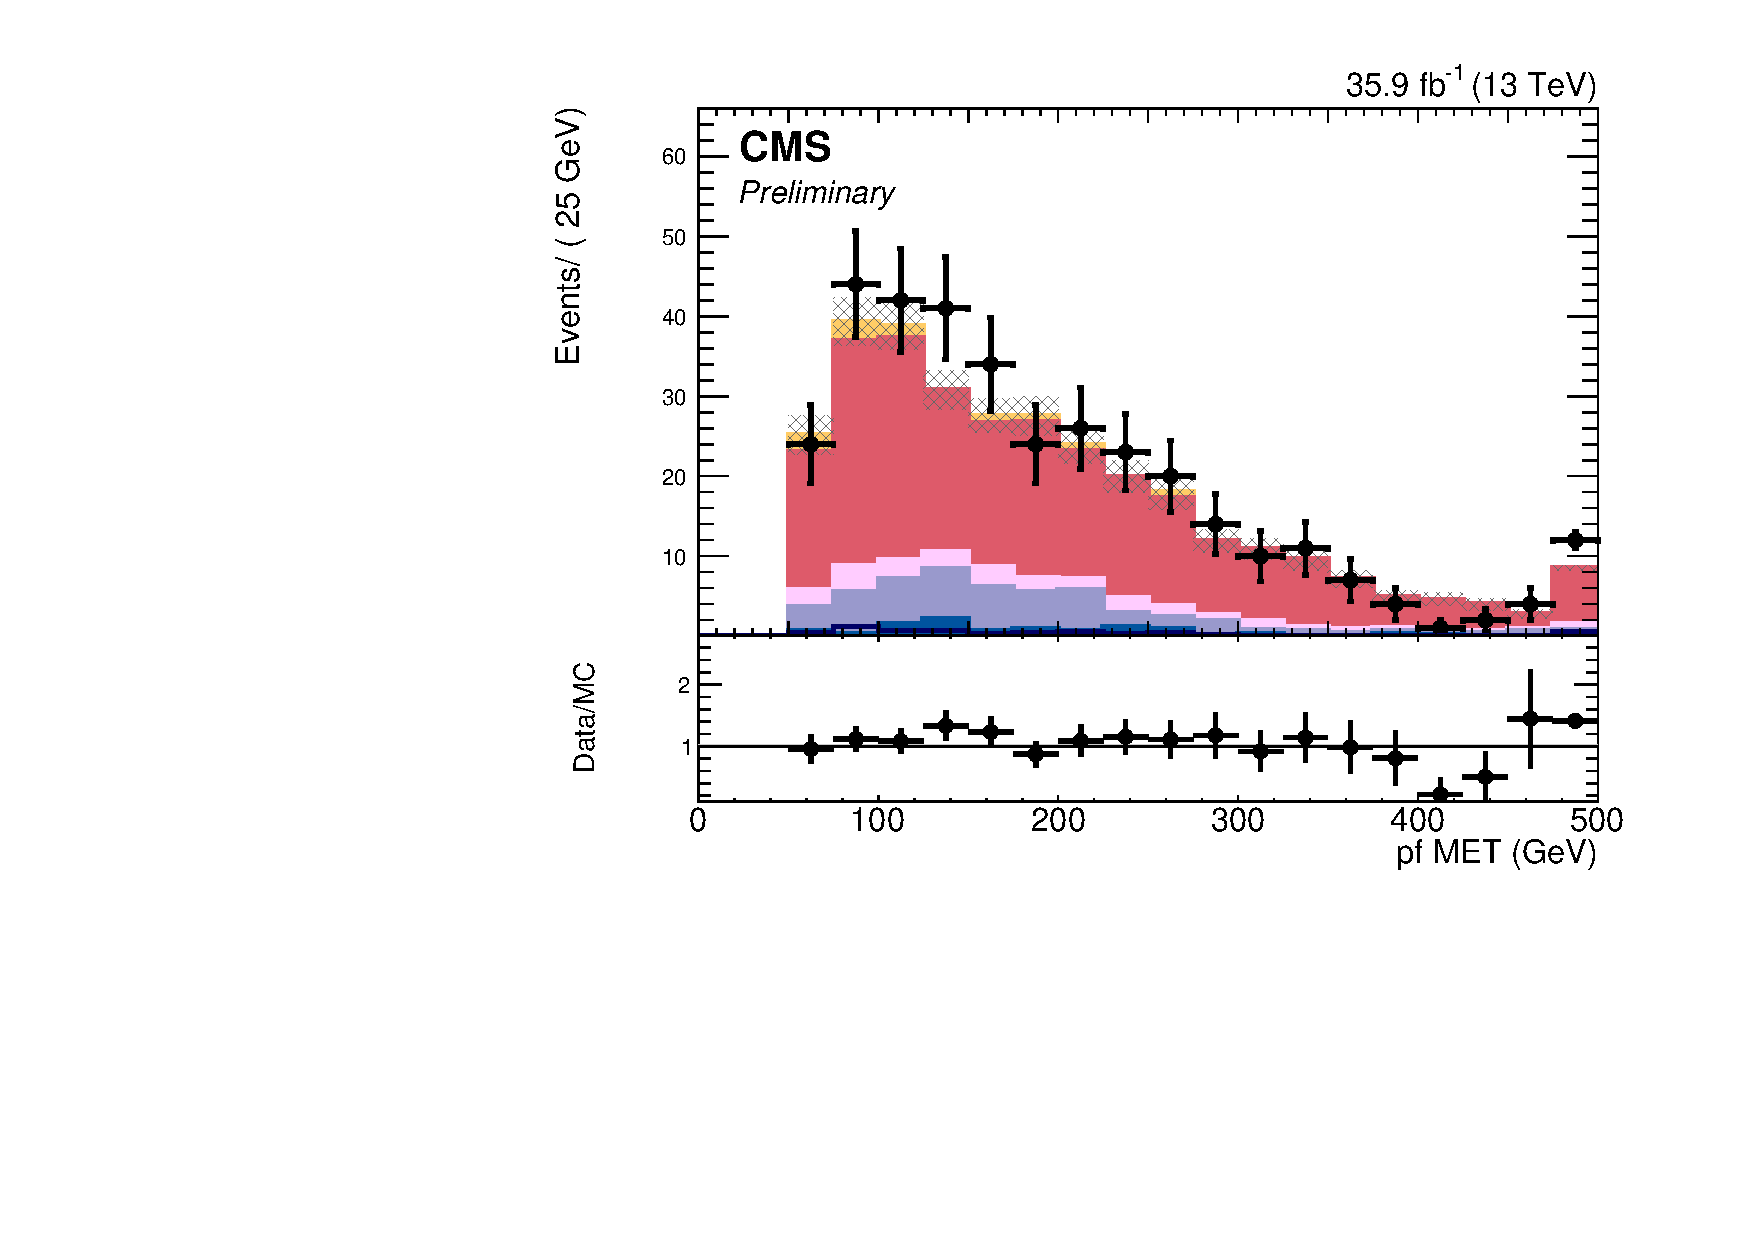
\includegraphics[width=0.45\textwidth]{Plots/plots/DibosonBoostedElMuCuts13TeV_WjetControlRegion_Tighter_CHS_pfMET_Corr.pdf}%
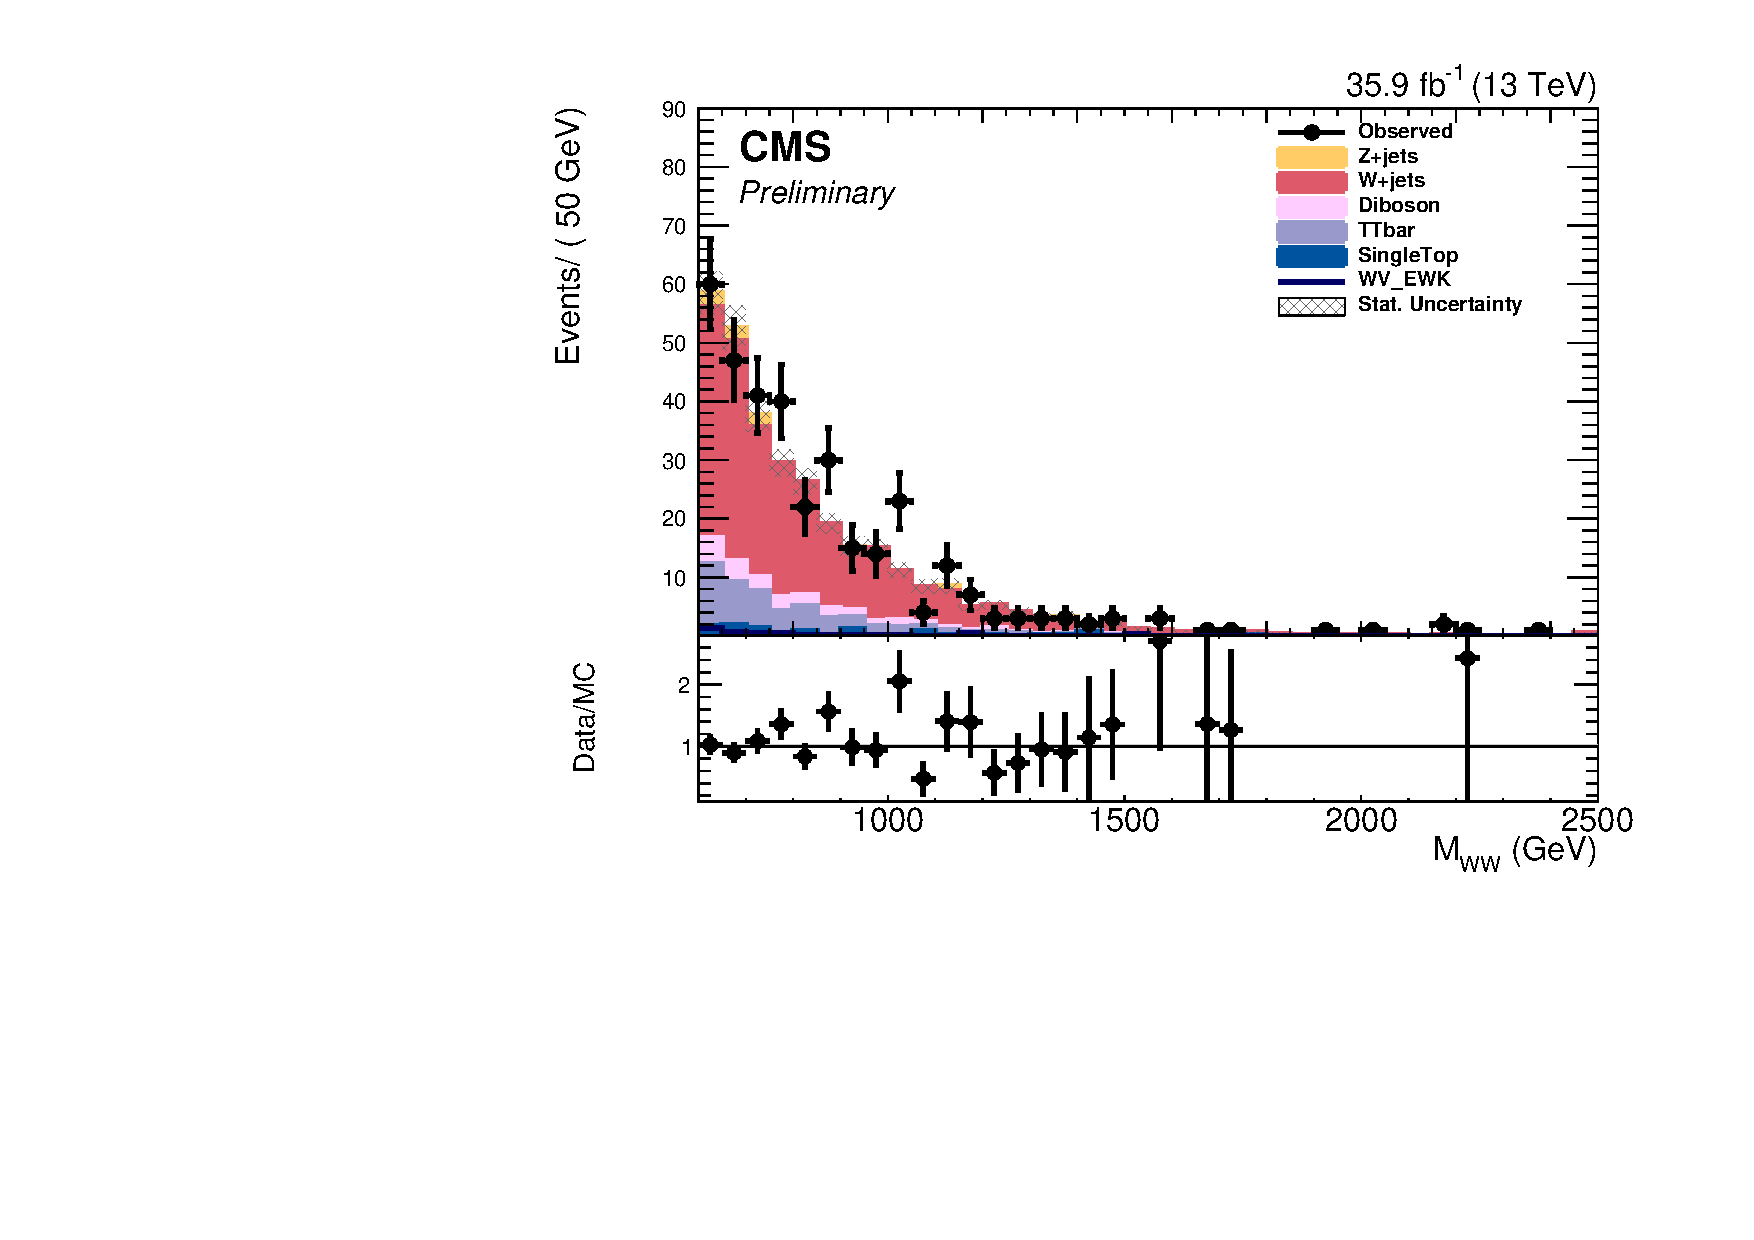
\includegraphics[width=0.45\textwidth]{Plots/plots/DibosonBoostedElMuCuts13TeV_WjetControlRegion_Tighter_CHS_mass_lvj_type0_PuppiAK8.pdf}\\
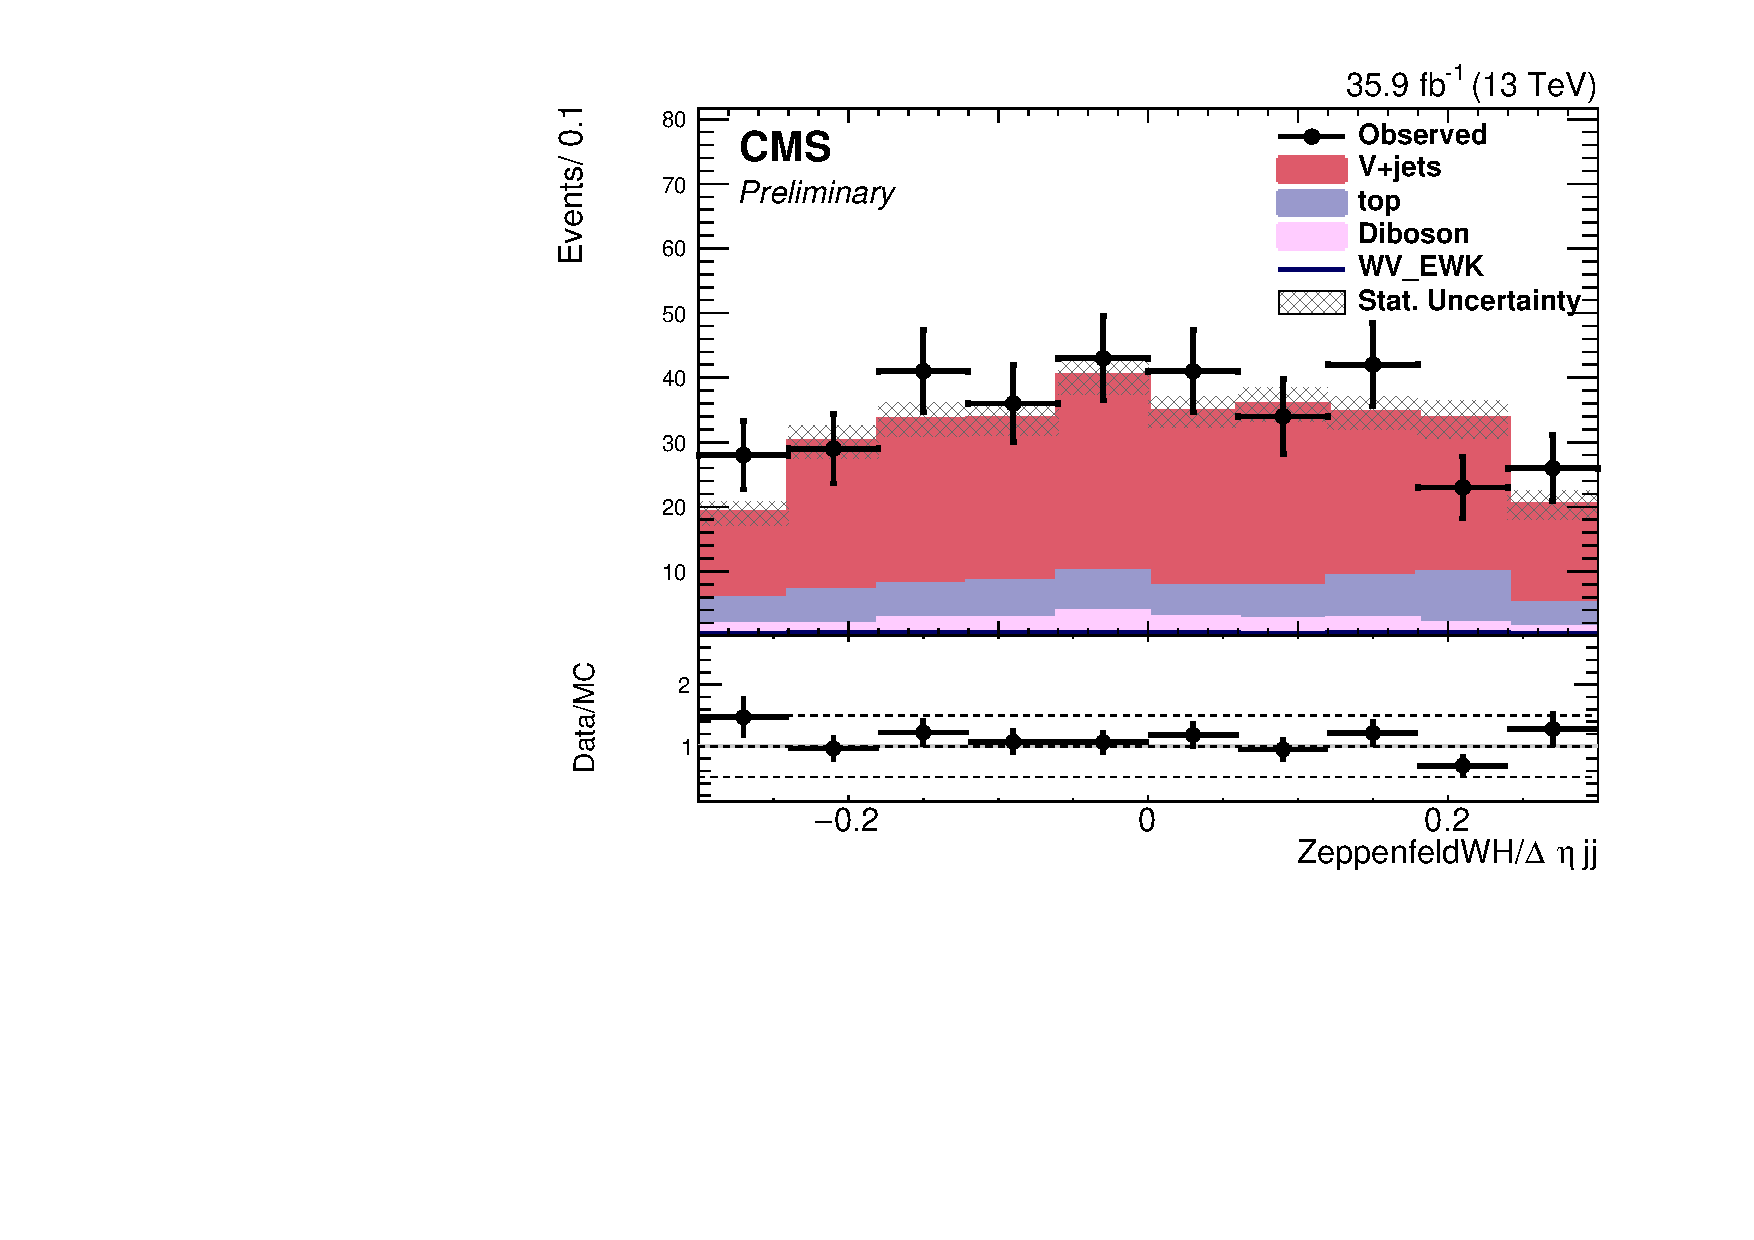
\includegraphics[width=0.45\textwidth]{Plots/plots/DibosonBoostedElMuCuts13TeV_WjetControlRegion_Tighter_CHS_ZeppenfeldWH_new.pdf}%
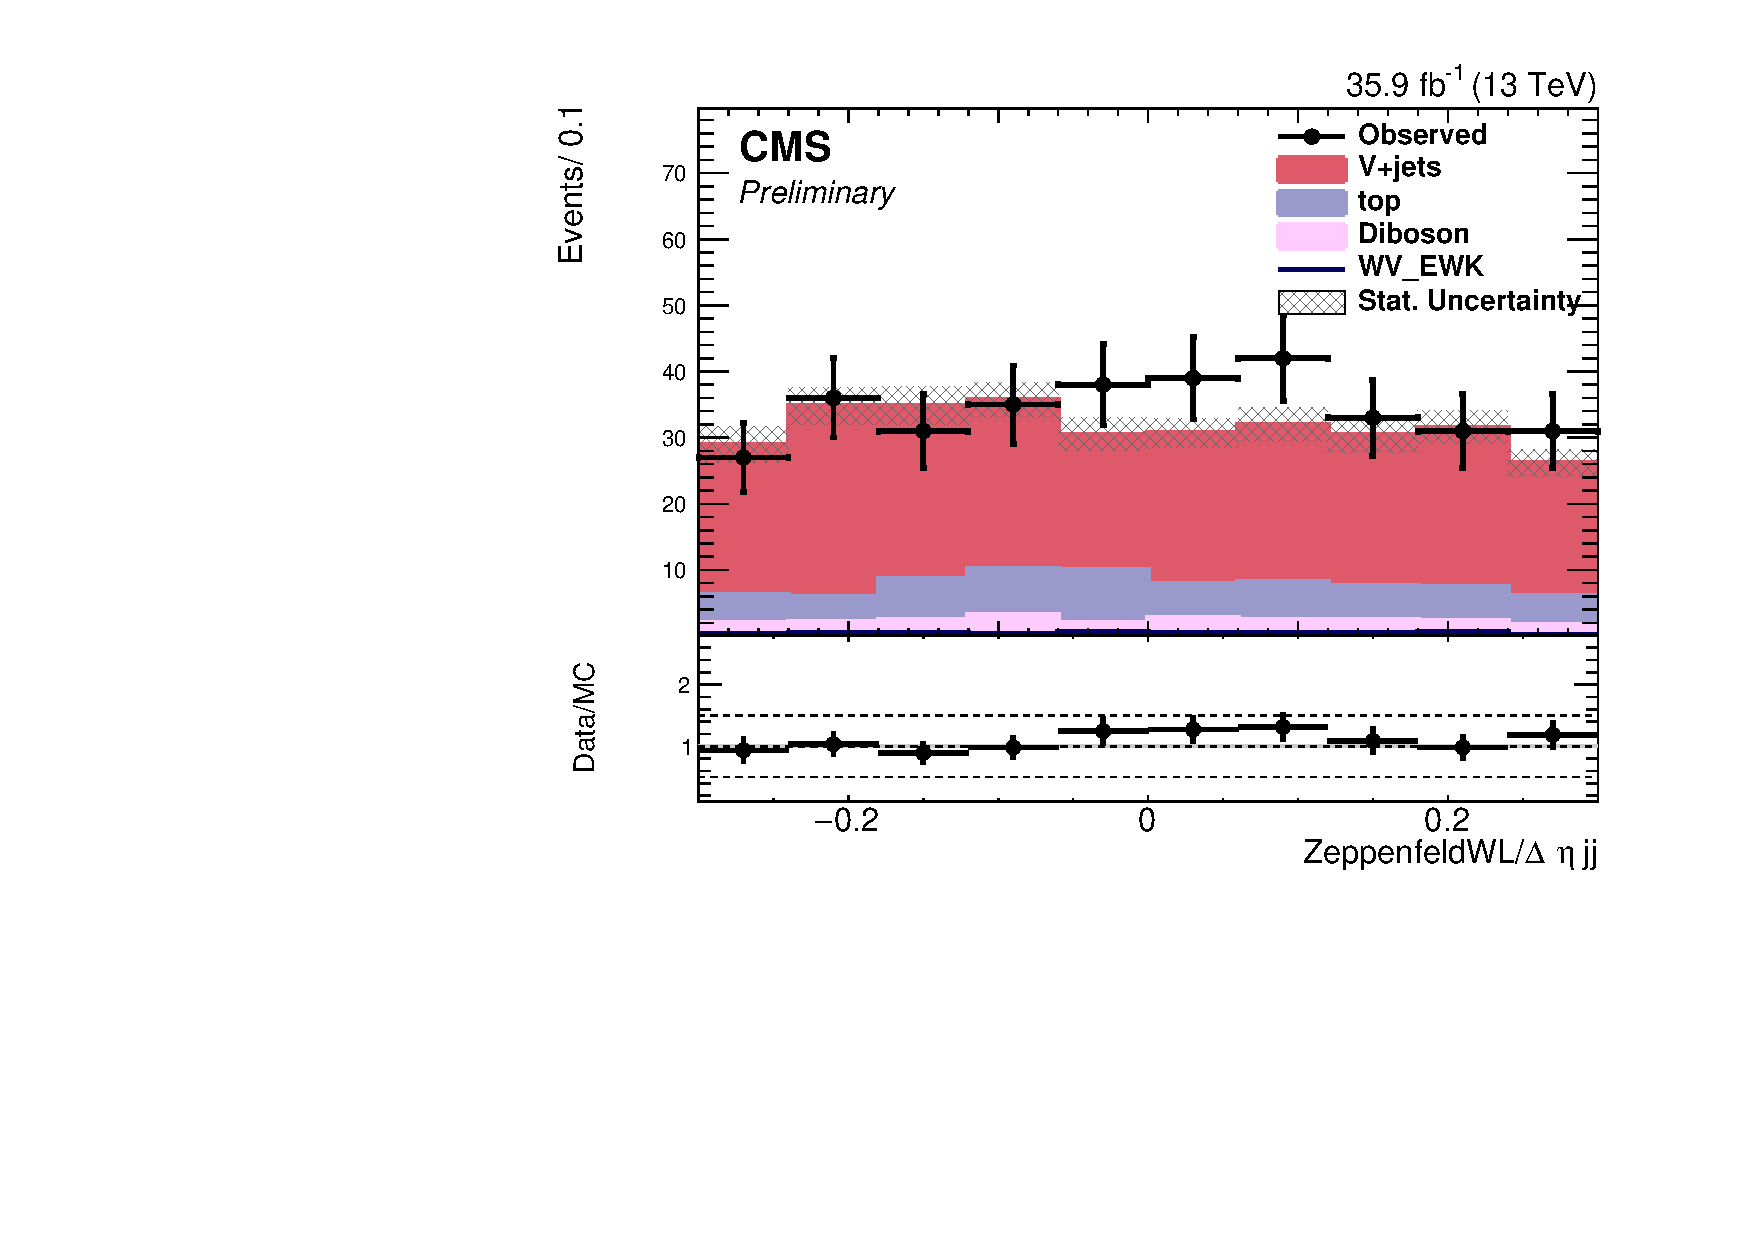
\includegraphics[width=0.45\textwidth]{Plots/plots/DibosonBoostedElMuCuts13TeV_WjetControlRegion_Tighter_CHS_ZeppenfeldWL_type0_new.pdf}\\
% 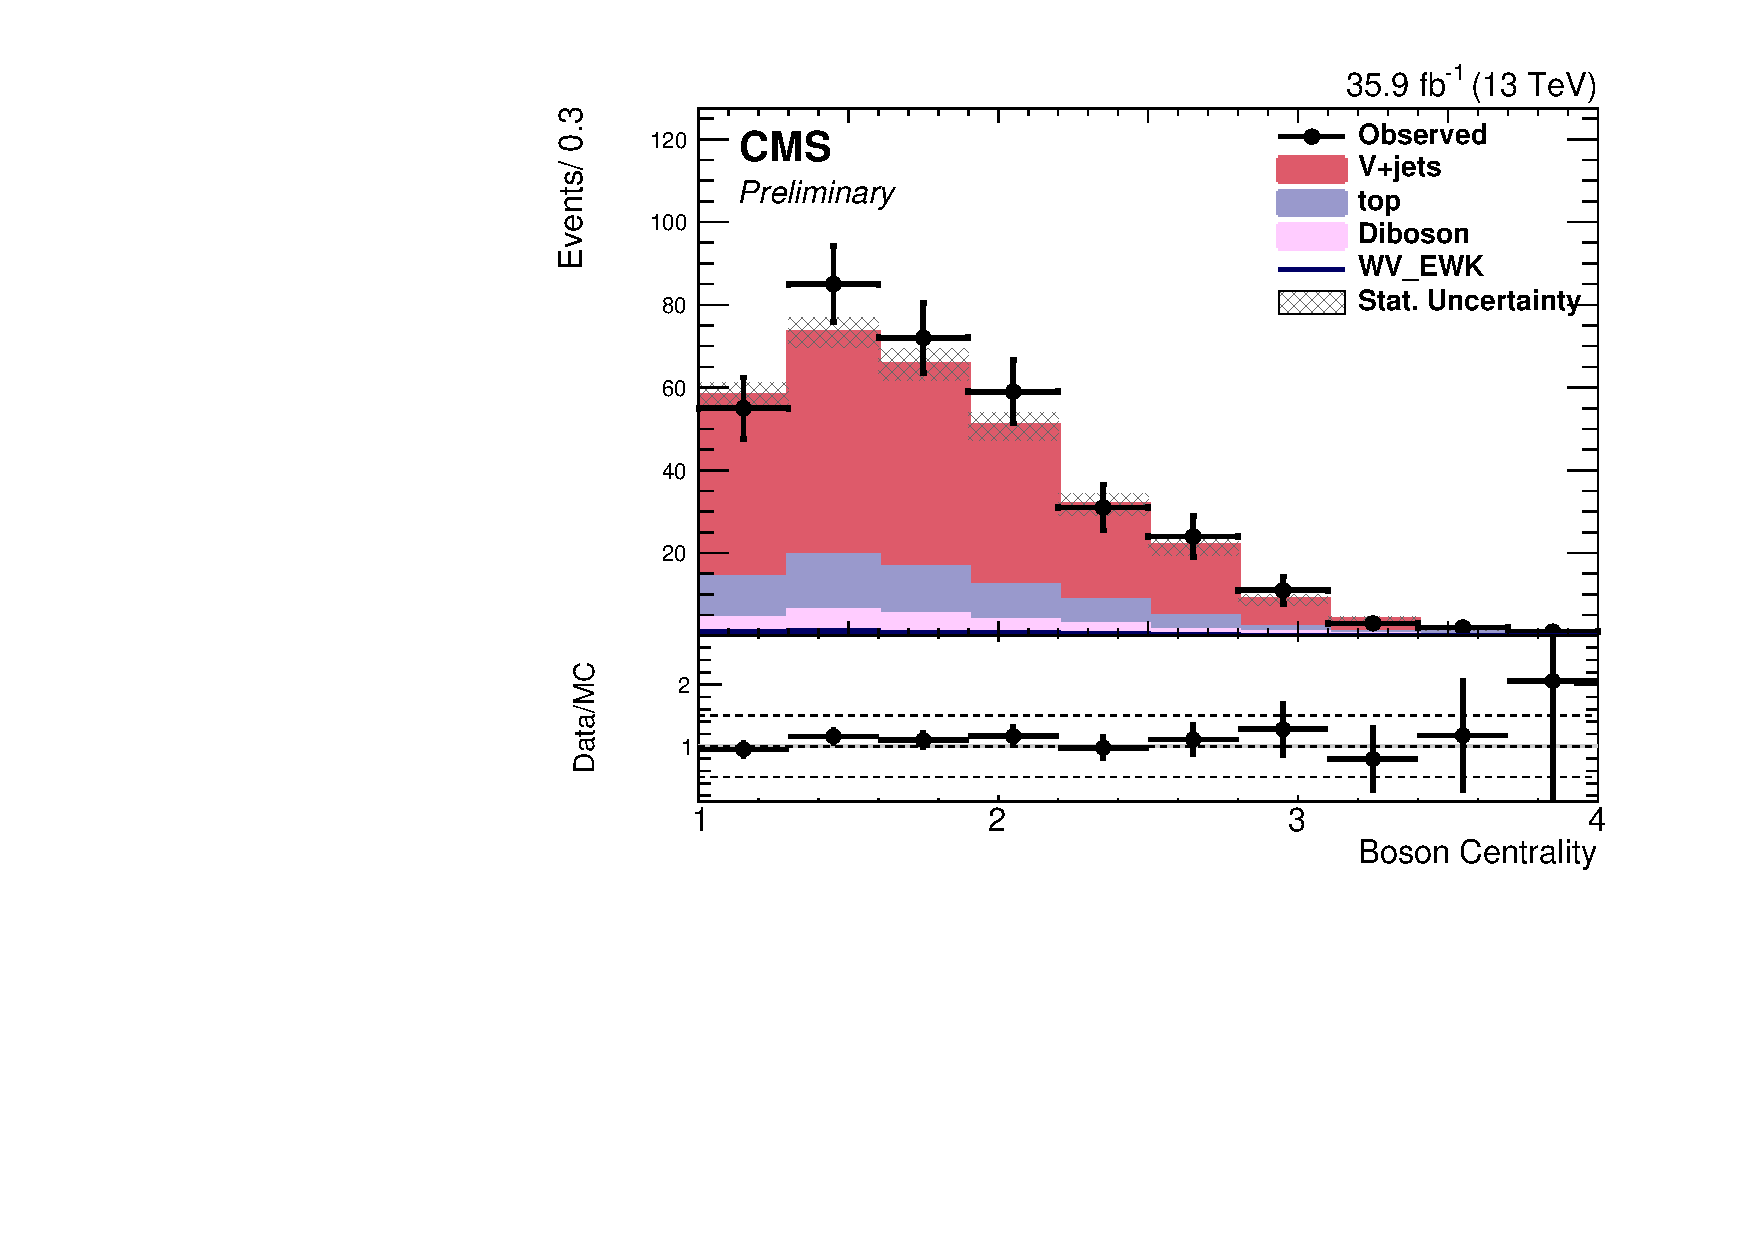
\includegraphics[width=0.45\textwidth]{Plots/plots/DibosonBoostedElMuCuts13TeV_WjetControlRegion_Tighter_CHS_BosonCentrality_type0.pdf}
\caption{Kinematic distributions in the $W+$jets background sideband region. $W+$jets predictions are taken from the simulation. The hatched bands include statistical uncertainties from the predicted yields.}
\label{fig:wjet_control2}
\end{figure*}

The $W+$jet predictions from the simulation are not used in the statistical analysis of the event yields. The shape and normalization of this background are extracted from data in the sideband region given above. The background estimation described below closely follows the method used in previous inclusive searches in $W V$ final state~\cite{resonances,cmsnote}. More detailed description of the method can be found in the references. 

The AQGC limits are extracted using a fit to the $m_{WV}$ distribution in the $W V$ final state. The prediction of the $W+$jets background is obtained by performing a fit to the $m_{WV}$ distribution in the sideband region. The extrapolation factors (denoted as alpha-ratio values) to the signal region are obtained from the $W+$jet simulation as a function of the $m_{WV}$ variable as described below.   

The shapes of the $t\bar{t}$, single top, diboson, and $W+$jet processes are represented by parametric shapes extracted from simulation. The following parametric functions are used: 

\begin{description}
	\item [Main function] $f_{ExpTail} = \exp(\frac{-x}{a+bx})$
	\item [Alternate Function] $f_{Exp} = \exp(cx)$
\end{description}

The resulting shapes are shown in Figure~\ref{fig:mWW_1}. The shown error band is determined by evaluating the fitted functions many times for several points along the x axis with the fitted parameters randomized according to their resulting uncertainty. The extracted fit parameters are summarized in Table~\ref{Table:BackgroundEstimation_mWWFitPars}. These templates are then used to fit the $m_{WV}$ distribution in the sideband region. The normalization and shape of the  $W$+jets process is floated in the fit. The other background processes are fixed to the SM predictions. The resulting fit is shown in Figure~\ref{fig:DataMCForMWW}.

\begin{figure}[htbp] 
	 \centering 
	 \begin{tabular}{cc}
	 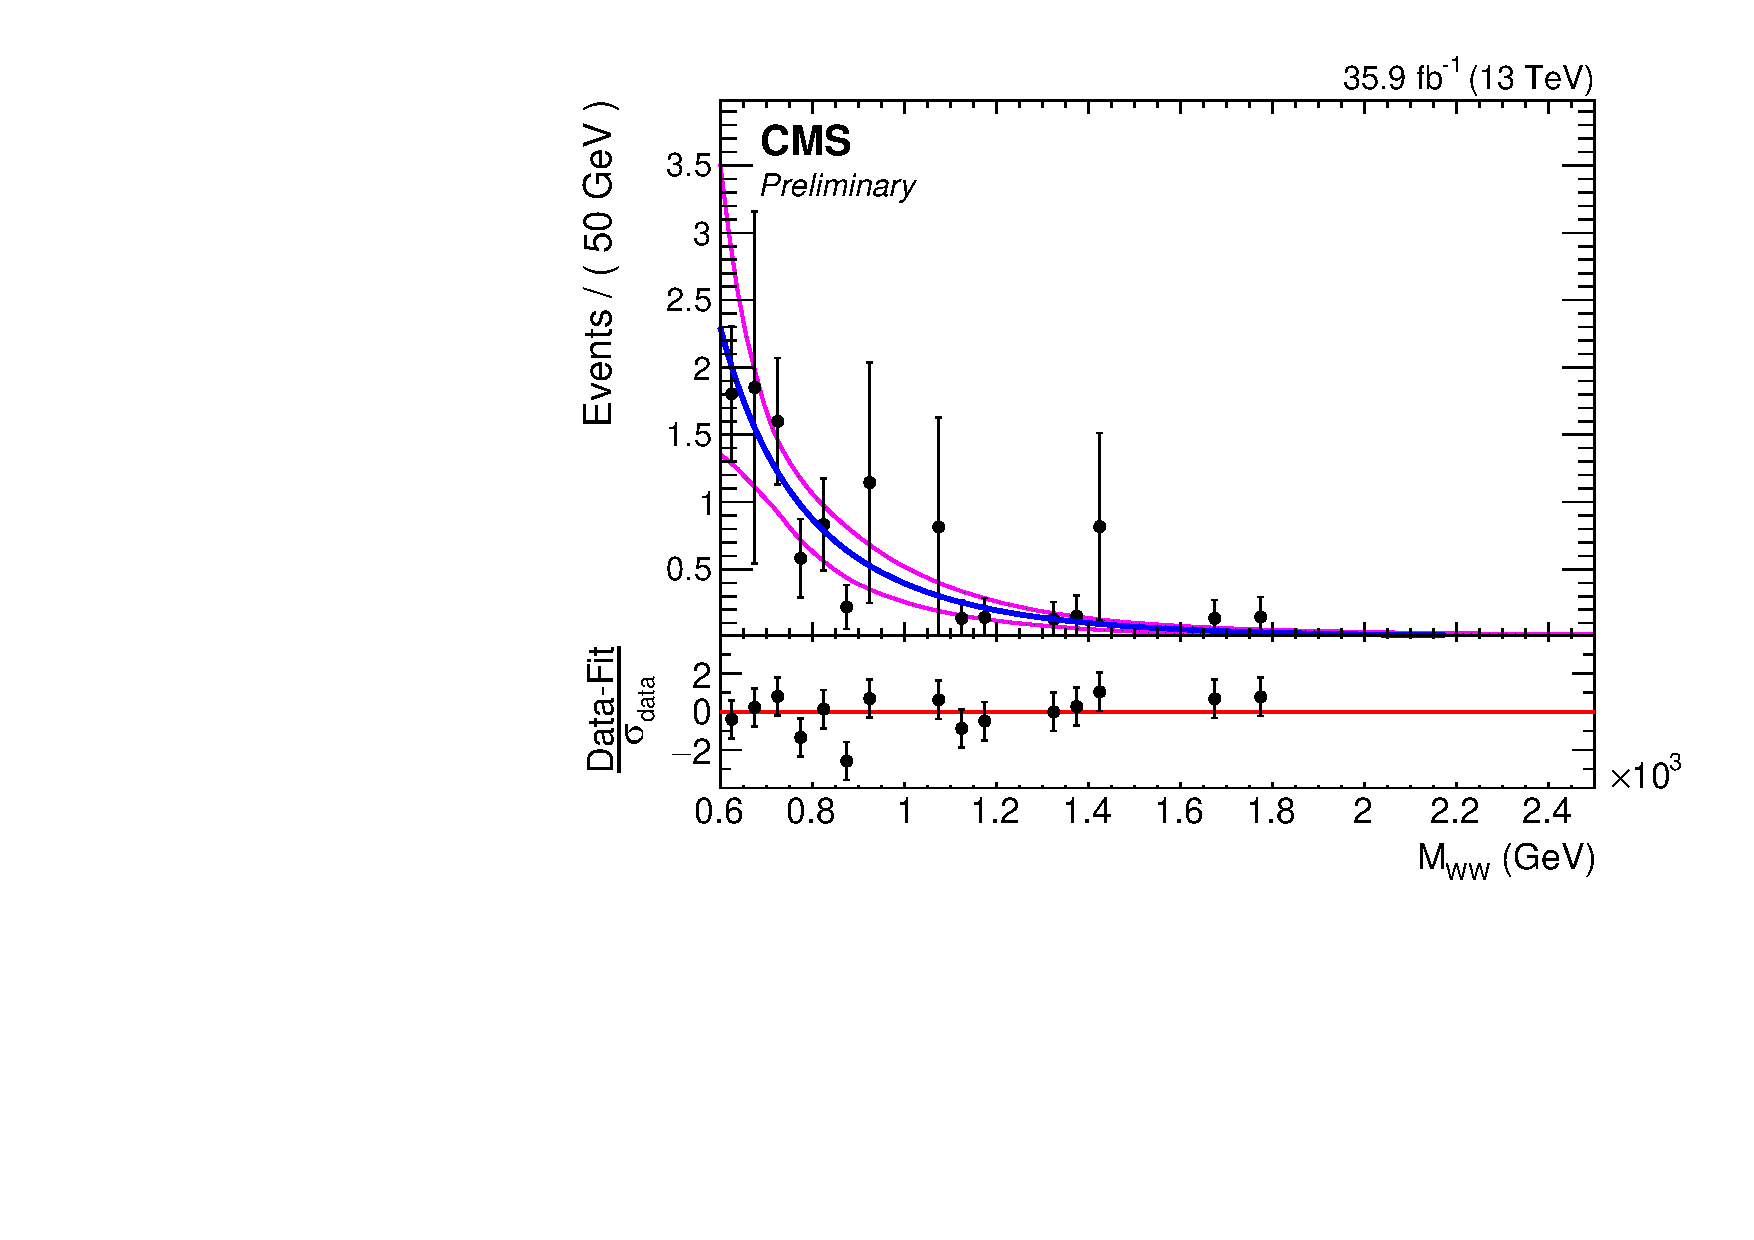
\includegraphics[width=0.48\textwidth]{Plots/BackgroundEstimation/WV/m_lvj_fitting/WWTree_STop_m_lvj_sb_loExpN_with_pull.pdf}
	 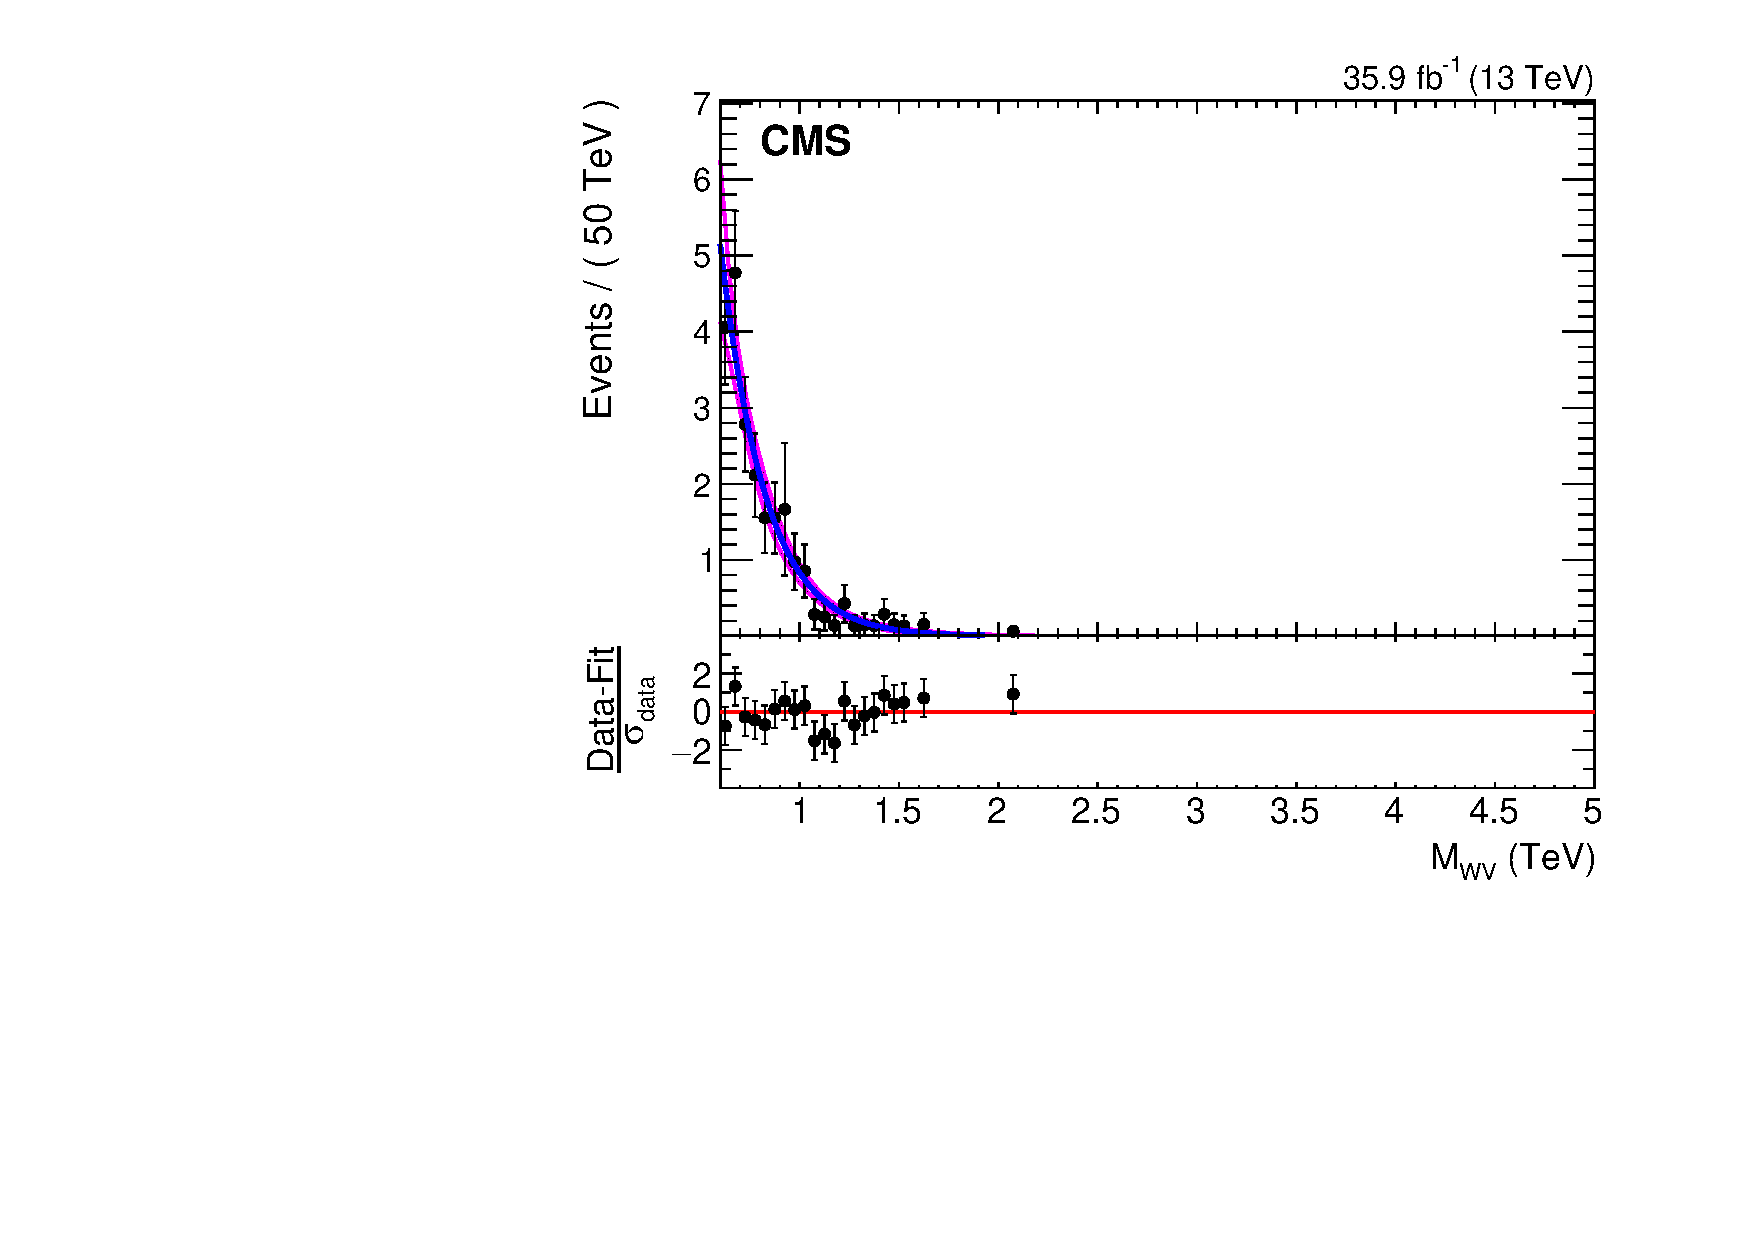
\includegraphics[width=0.48\textwidth]{Plots/BackgroundEstimation/WV/m_lvj_fitting/WWTree_STop_m_lvj_signal_regionExpN_with_pull.pdf}\\
	 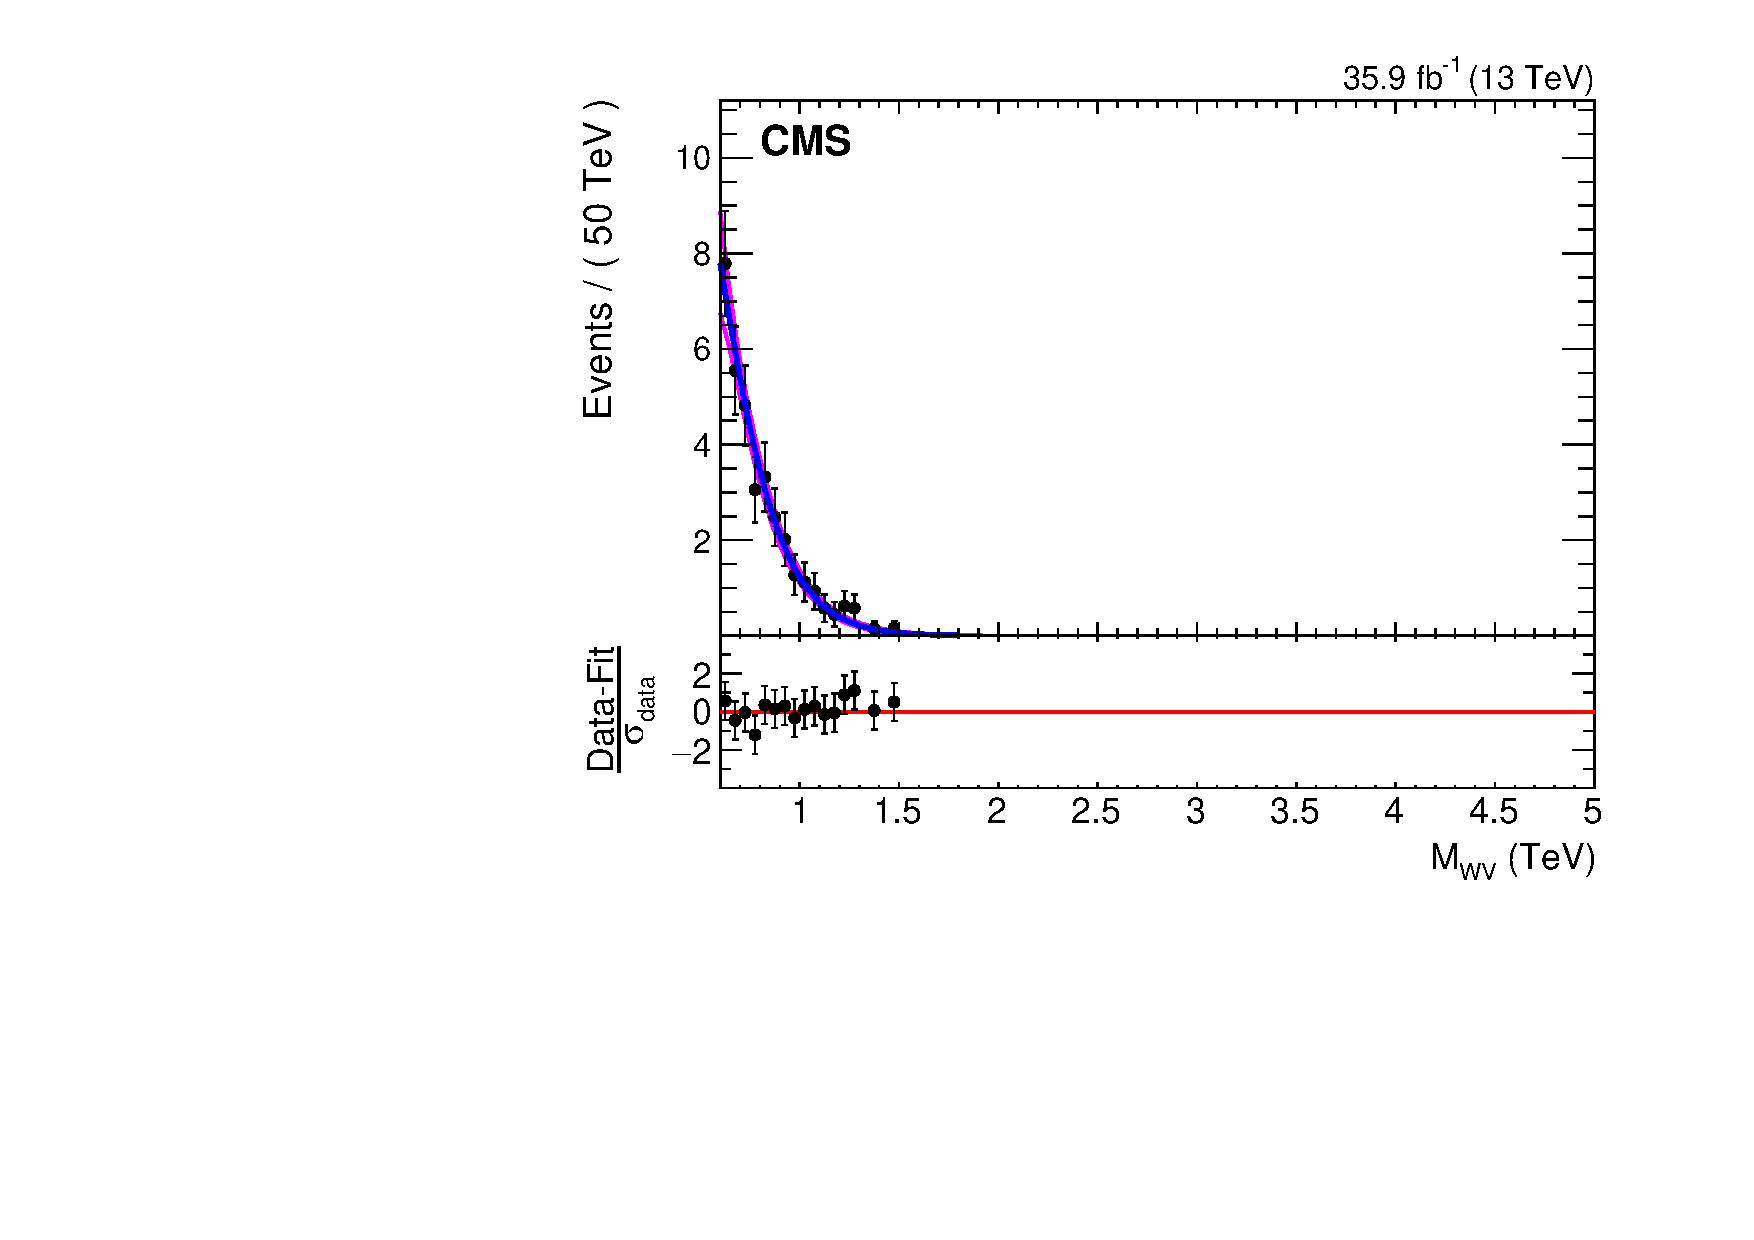
\includegraphics[width=0.48\textwidth]{Plots/BackgroundEstimation/WV/m_lvj_fitting/WWTree_TTbar_m_lvj_sb_loExpN_with_pull.pdf}
	 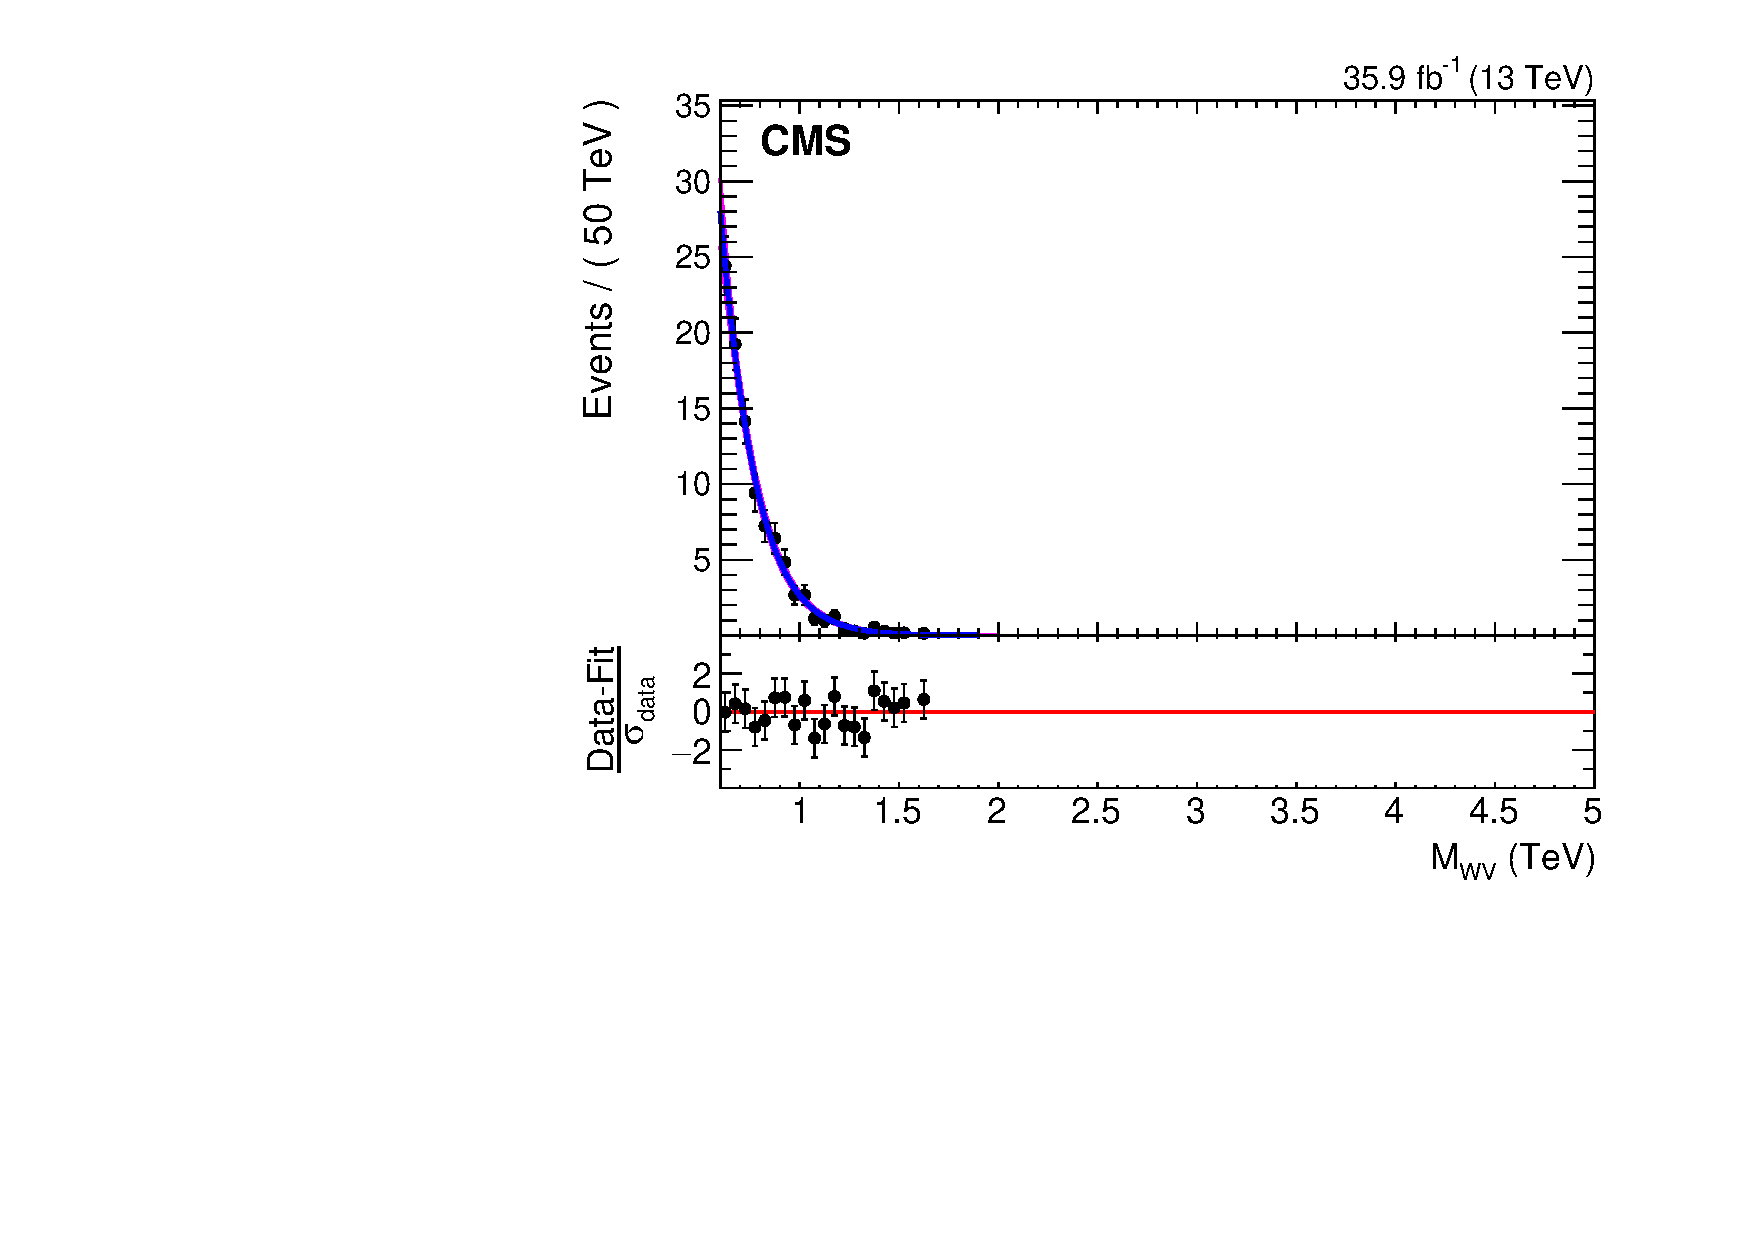
\includegraphics[width=0.48\textwidth]{Plots/BackgroundEstimation/WV/m_lvj_fitting/WWTree_TTbar_m_lvj_signal_regionExpN_with_pull.pdf}\\
	 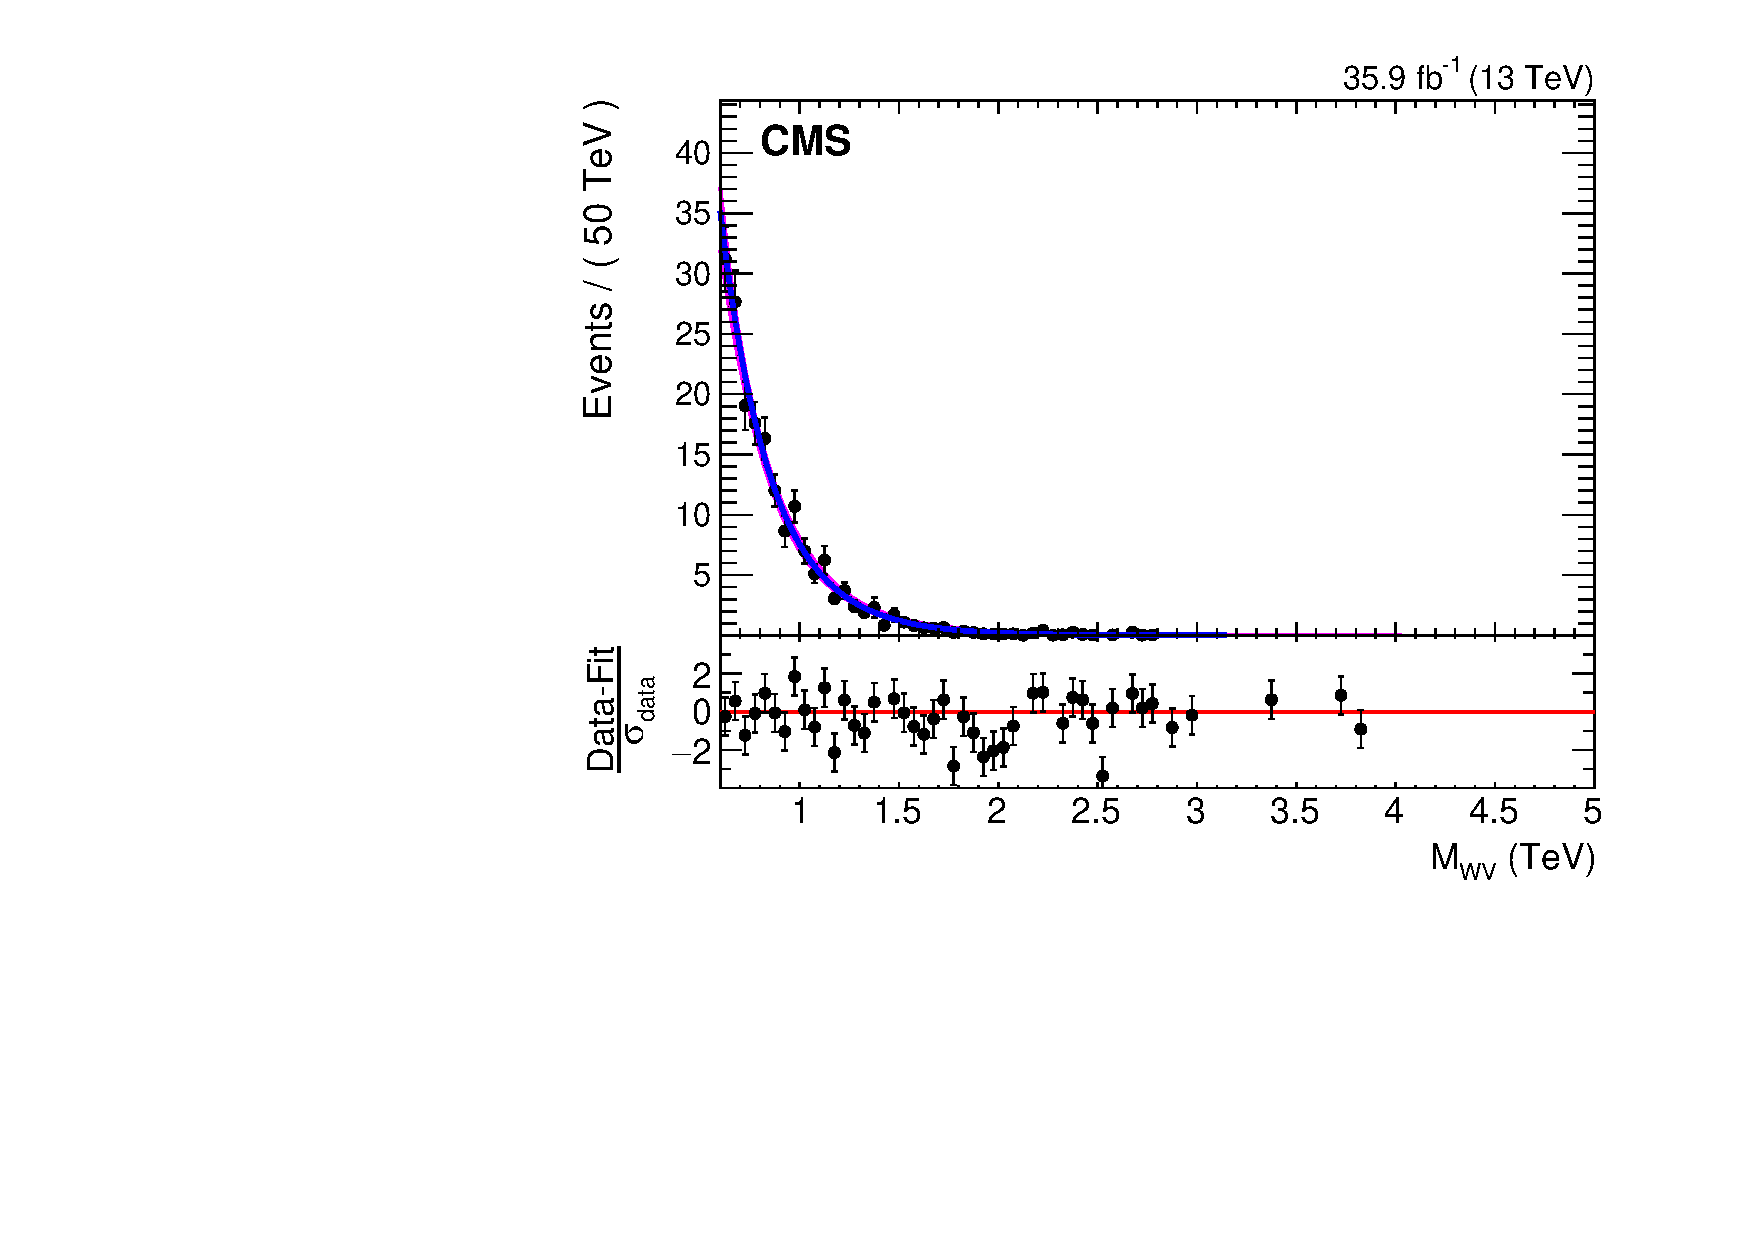
\includegraphics[width=0.48\textwidth]{Plots/BackgroundEstimation/WV/m_lvj_fitting/WWTree_VJets_m_lvj_sb_loExpTail_with_pull.pdf}
	 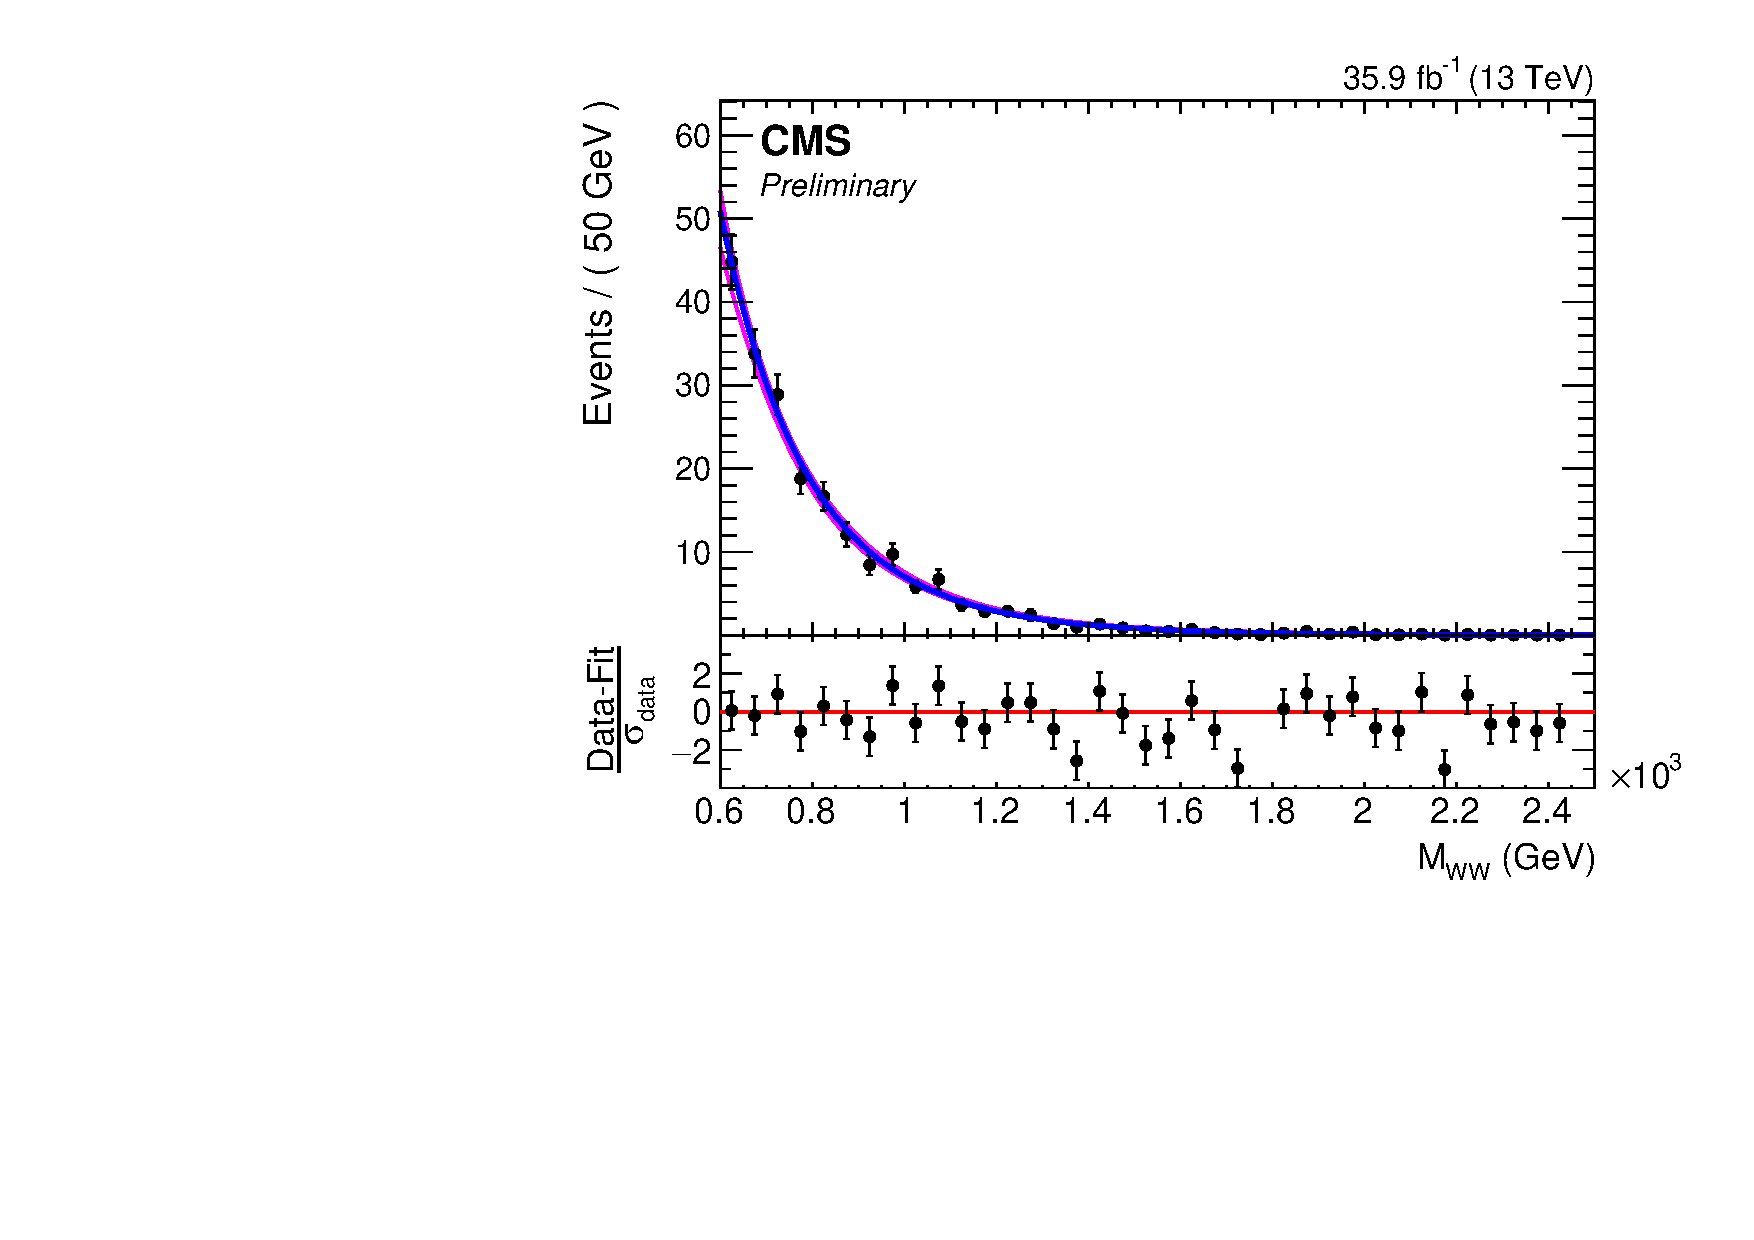
\includegraphics[width=0.48\textwidth]{Plots/BackgroundEstimation/WV/m_lvj_fitting/WWTree_VJets_m_lvj_signal_regionExpTail_with_pull.pdf}\\
	 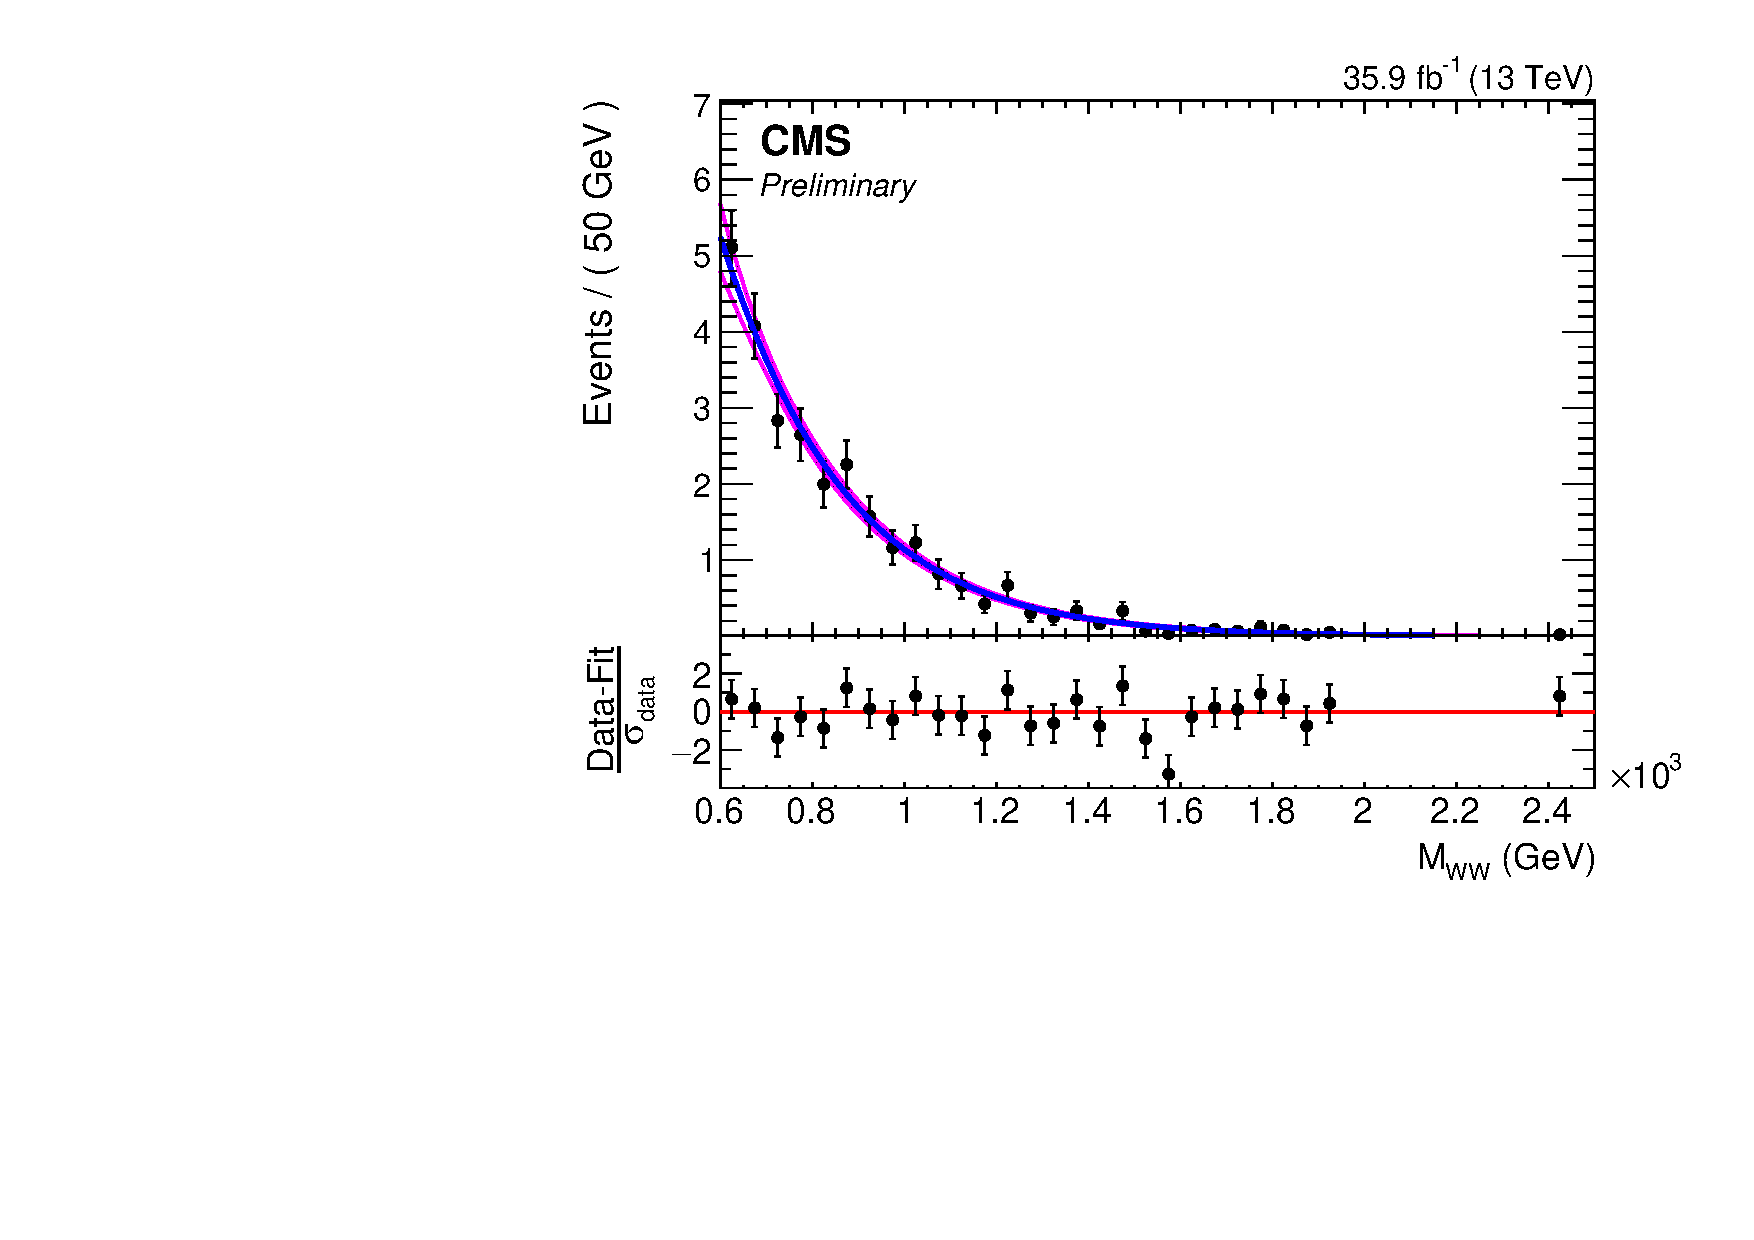
\includegraphics[width=0.48\textwidth]{Plots/BackgroundEstimation/WV/m_lvj_fitting/WWTree_VV_EWK_QCD_m_lvj_sb_loExpN_with_pull.pdf}
	 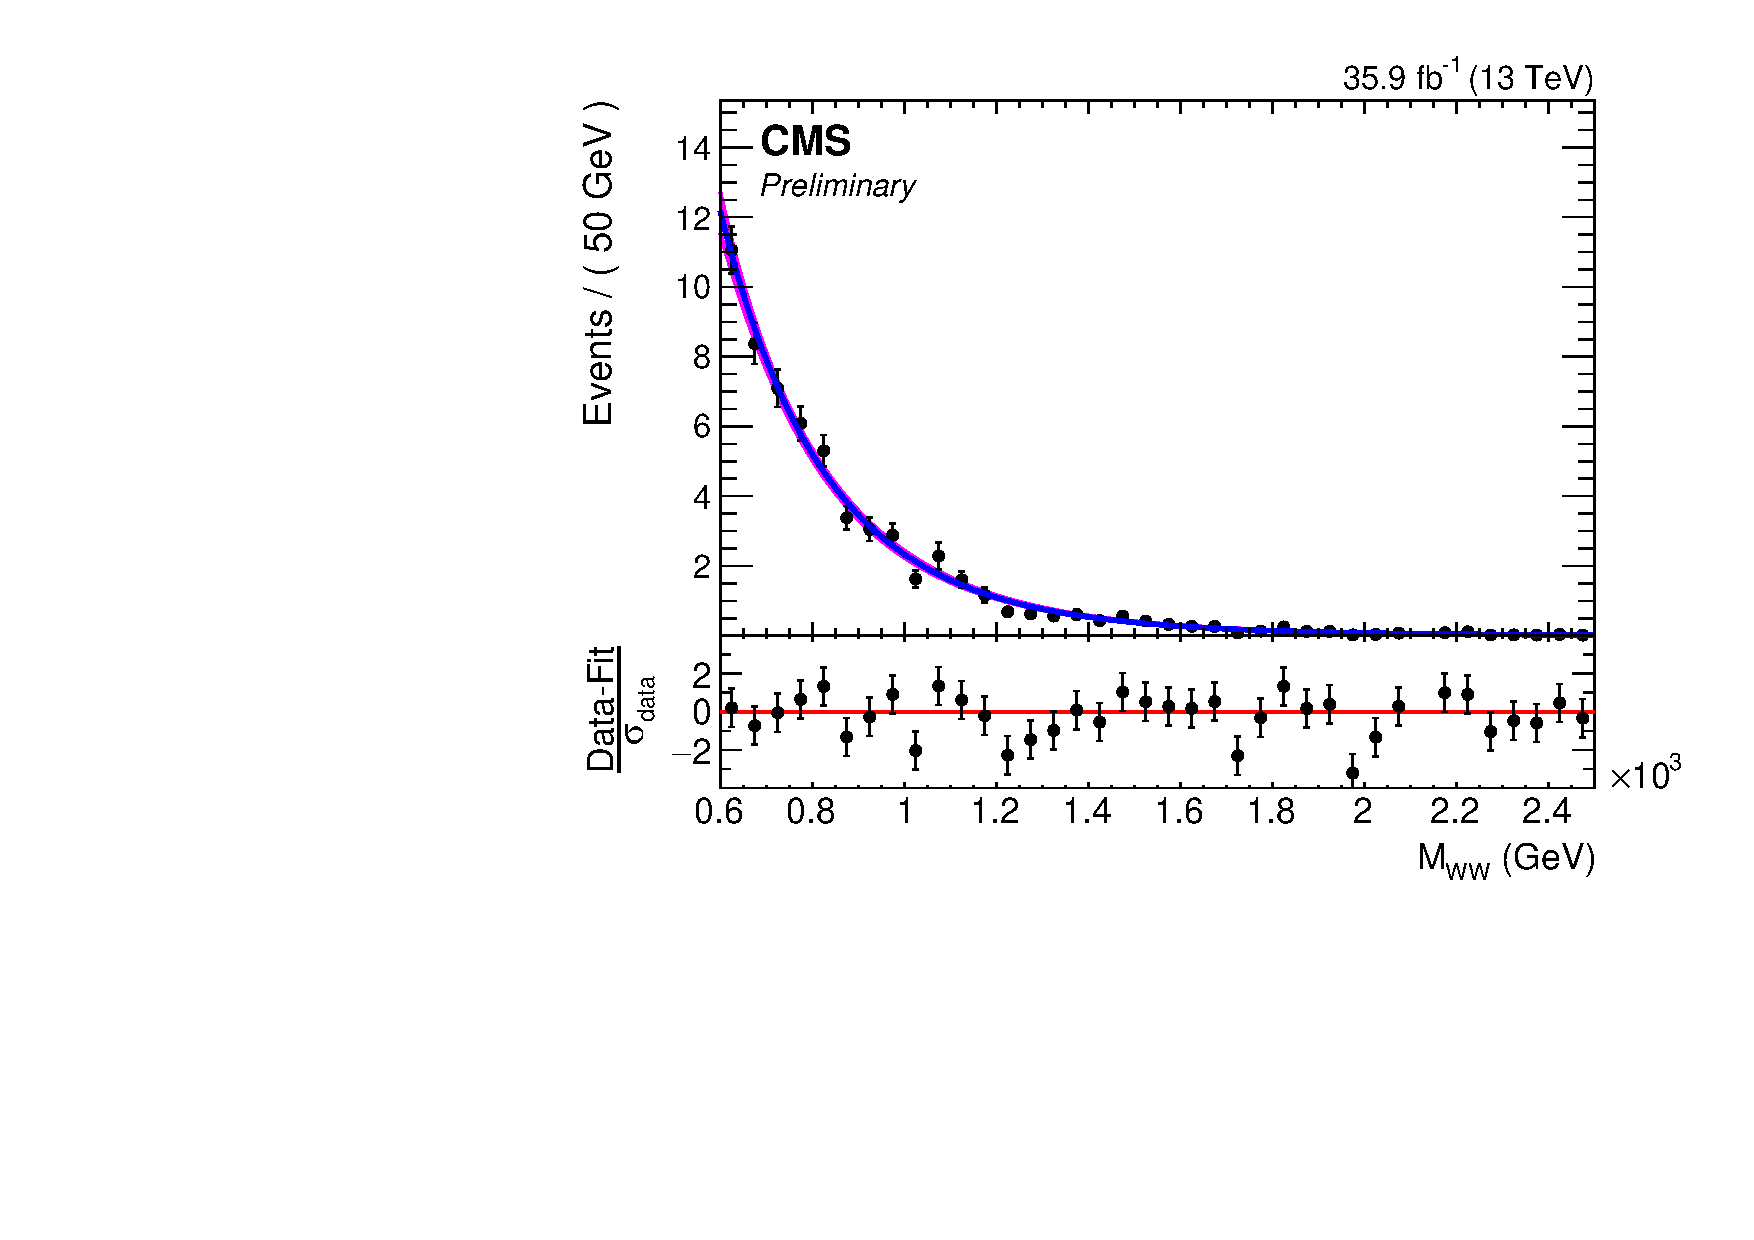
\includegraphics[width=0.48\textwidth]{Plots/BackgroundEstimation/WV/m_lvj_fitting/WWTree_VV_EWK_QCD_m_lvj_signal_regionExpTail_with_pull.pdf}
	 \end{tabular}
	 \caption{MC-data and fit shape $m_{WV}$ distributions in the sideband (left) and signal regions (right). From top to bottom: single top, $t\bar{t}$, $W+$jets and dibosons.}
	 \label{fig:mWW_1}
\end{figure}

\begin{table}[h!]
	\centering
	\begin{tabular}{||c | c||} 
	 \hline
	 parameter & Values \\
	 \hline \hline
	 \multicolumn{2}{|c|}{W+jets, $f_{ExpTail}$}\\
	 \hline
	 a 			&	0.0360242 $\pm$ 0.0259207\\
	 b 			&	196.282	$\pm$ 69.6708\\
	 $N$ 		&	240.834 $\pm$ 17.9165\\
	 \hline \hline
	 \multicolumn{2}{|c|}{W+jets (alternate function), $f_{Exp}$}\\
	 \hline
	 c 			&	-0.00349426 $\pm$ 0.000258006\\
	 $N$ 		&	240.69 $\pm$ 17.9176\\
	 \hline \hline
	 \multicolumn{2}{|c|}{Diboson, $f_{ExpN}$}\\
	 \hline
	 c 			&	-0.00415878 $\pm$ 0.000478786\\
	 n 			&	-203.63 $\pm$ 424.762\\
	 $N$ 		&	27.4306 $\pm$ 1.10149\\
	 \hline \hline
	 \multicolumn{2}{|c|}{TTbar, $f_{ExpN}$}\\
	 \hline
	 c 			&	-0.00671012 $\pm$ 0.00124636\\
	 n 			&	-983.791 $\pm$ 914.875\\
	 $N$ 		&	42.0095 $\pm$ 2.51186\\
	 \hline \hline
	 \multicolumn{2}{|c|}{Single Top, $f_{ExpN}$}\\
	 \hline
	 c 			&	-0.0026518 $\pm$ 0.00234551\\
	 n 			&	1045.48 $\pm$ 2235.03\\
	 $N$ 		&	10.5114 $\pm$ 2.11656\\
	 \hline \hline
	\end{tabular}
 	\caption{Extracted fit parameters for the functions describing the $m_{WV}$ distributions.}
 	\label{Table:BackgroundEstimation_mWWFitPars}
\end{table}


\begin{figure}[htbp] 
	 \centering 
	 \begin{tabular}{cc}
	 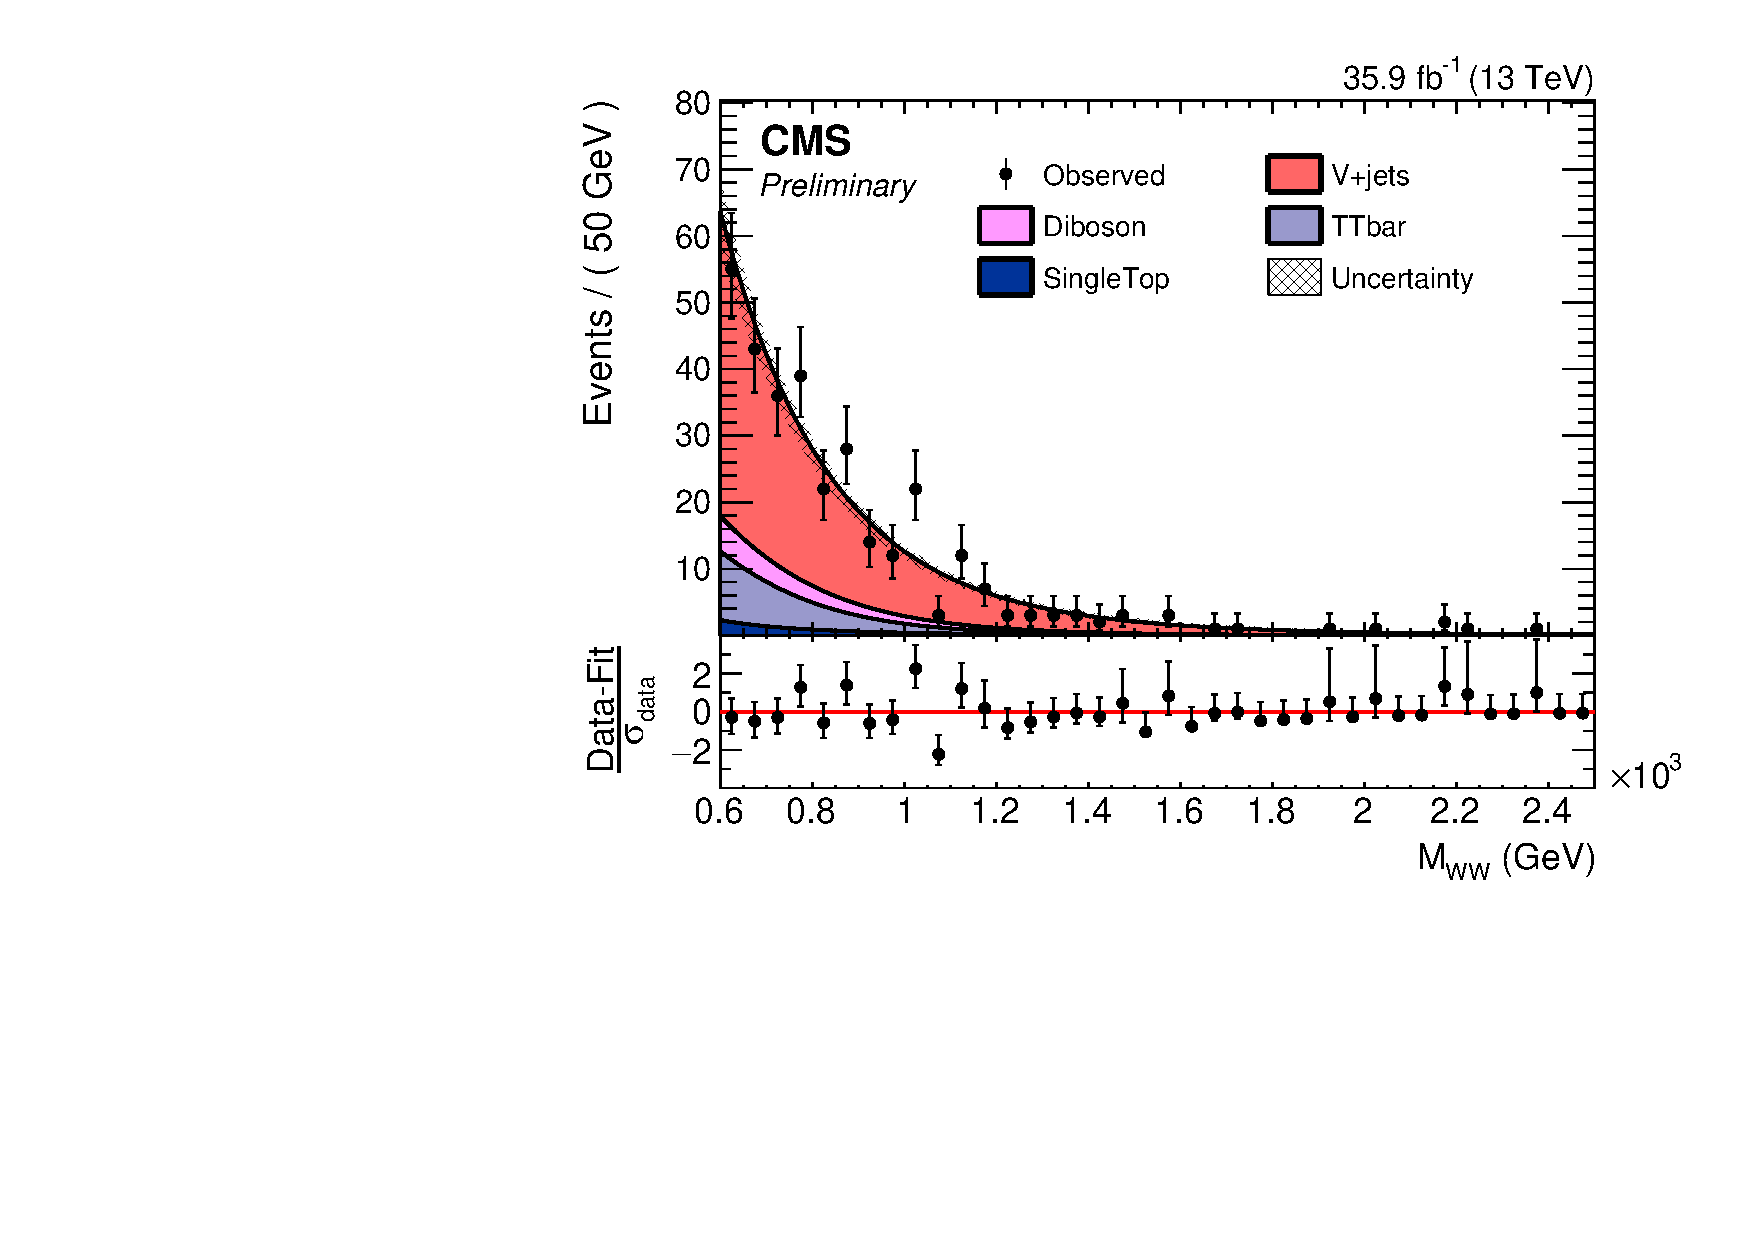
\includegraphics[width=0.48\textwidth]{Plots/BackgroundEstimation/WV/m_lvj_fitting/m_lvj_sb_lo_WJets0_xww__with_pull.pdf}
	 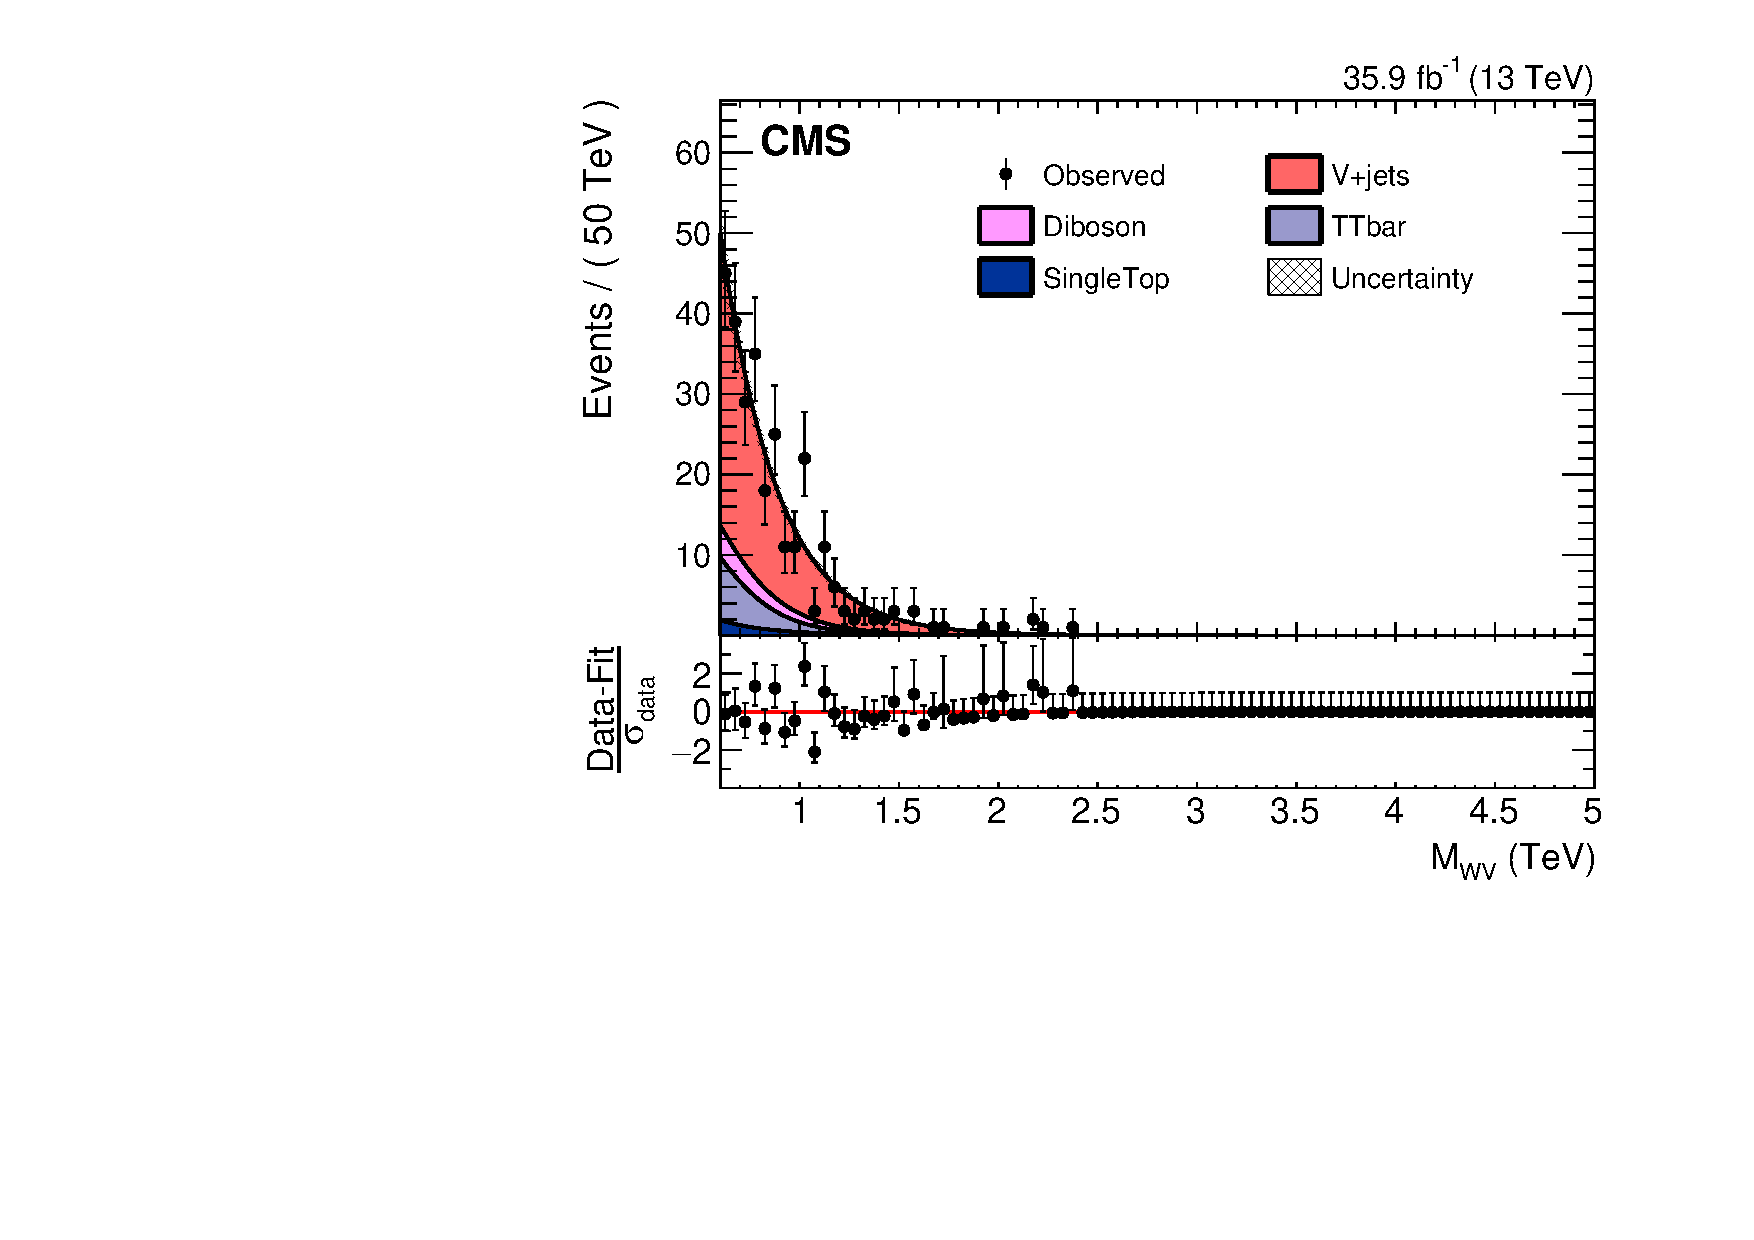
\includegraphics[width=0.48\textwidth]{Plots/BackgroundEstimation/WV/m_lvj_fitting/m_lvj_sb_lo_WJets01_xww__with_pull.pdf} 
	 \end{tabular}
	 \caption{The data distribution and the corresponding fit of the $m_{WV}$ distribution in the sideband region for the nominal parametric function (left) and a modified fparametric function (right).}
	 \label{fig:DataMCForMWW}
\end{figure}

 The contribution of the $W+$jet process in the signal region is obtained using the alpha-ratio-method~\cite{resonances,cmsnote}. The alpha-ratio values extrapolate the $W+$jet contribution from the sideband region to the signal region as a function of $m_{WV}$ using simulation. The resulting distribution is shown in Figure~\ref{fig:AlphaDis}. The statistical uncertainties are propagated to the result. The final $W+$jet prediction in the signal region is shown in Figure~\ref{fig:signal}. 

\begin{figure}[!htbp] 
	 \centering 
	 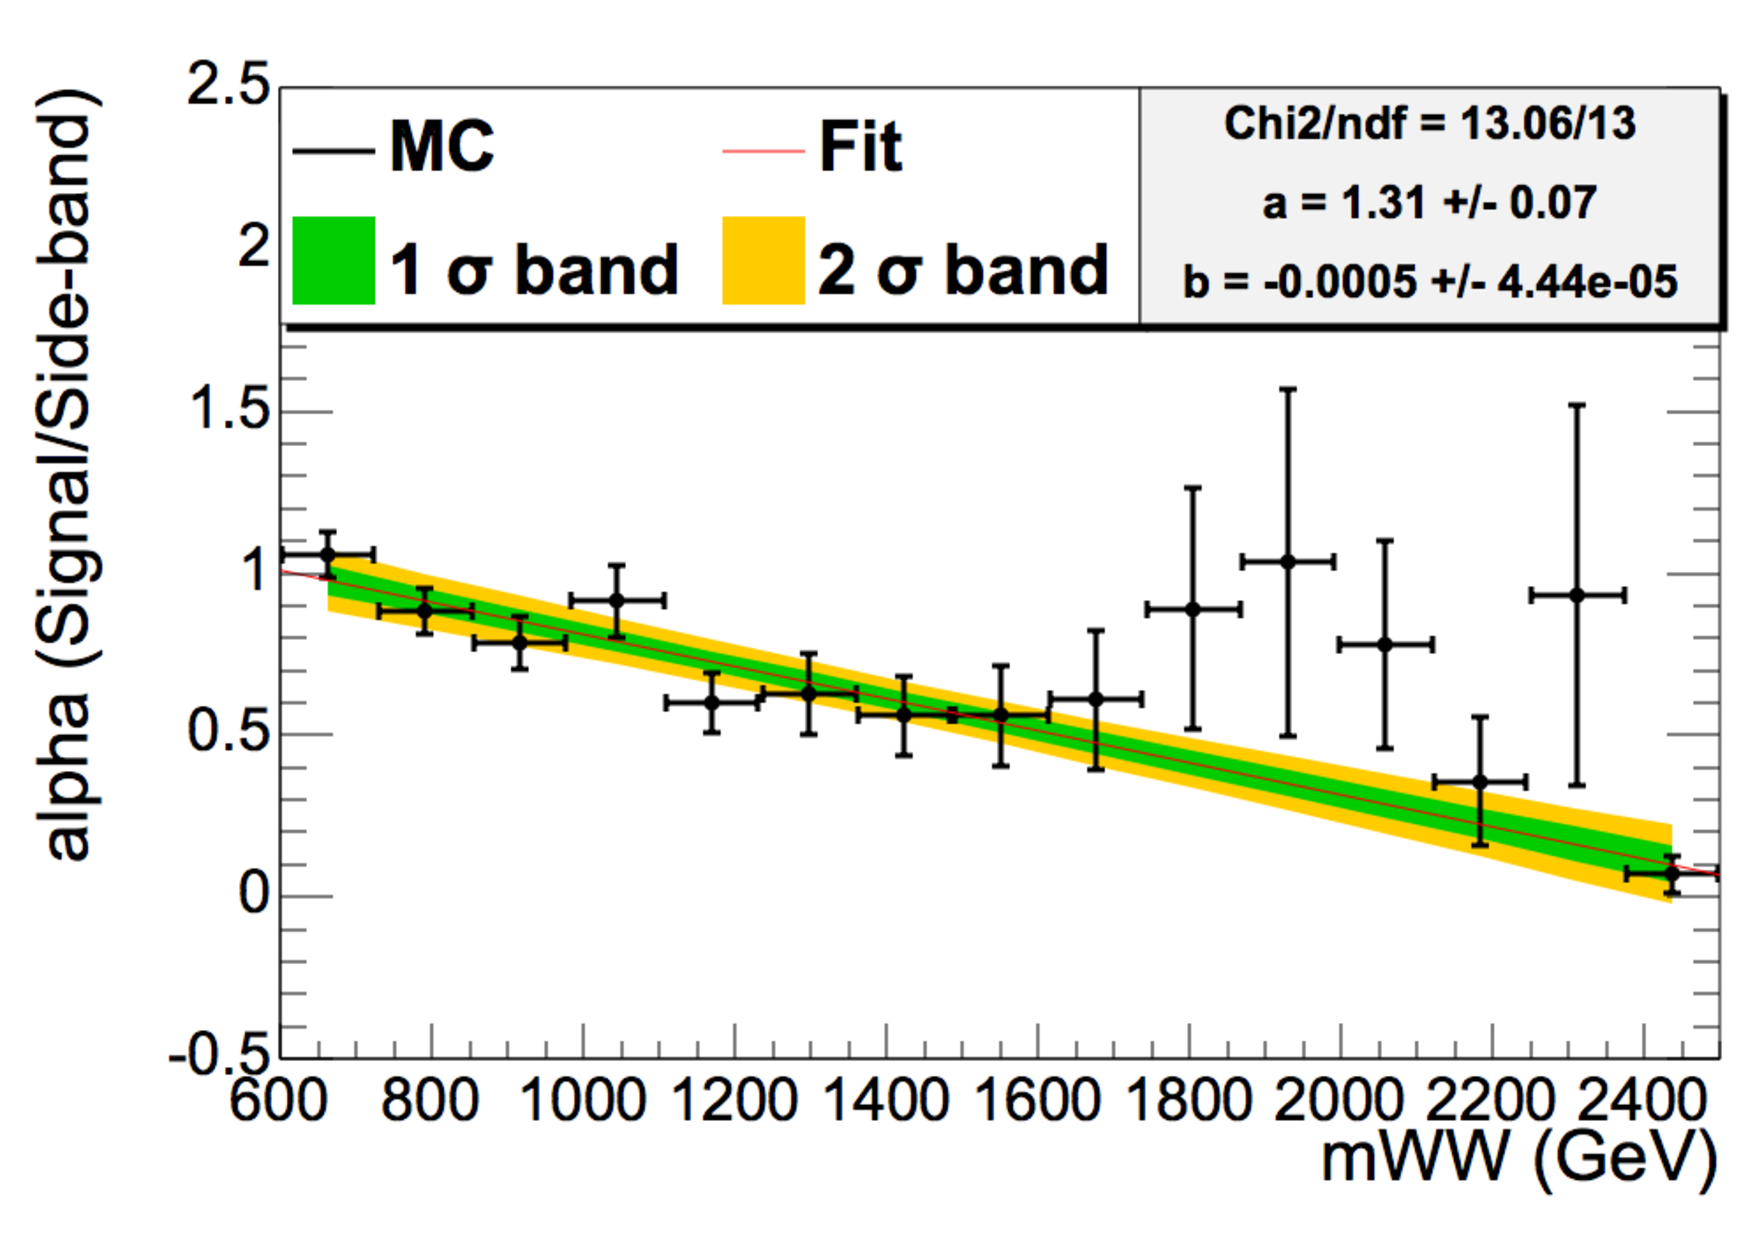
\includegraphics[width=0.48\textwidth]{Plots/BackgroundEstimation/WV/WVchannel_AlphaDistribution_AfterFit.pdf}
	 \caption{Alpha-ratio value (ratios of the $W+$jet MC contribution in the signal region to the sideband region) distribution. Red line is the fitted function used in the result.}
	 \label{fig:AlphaDis}
\end{figure}

\begin{figure}[h!] 
	 \centering 
	 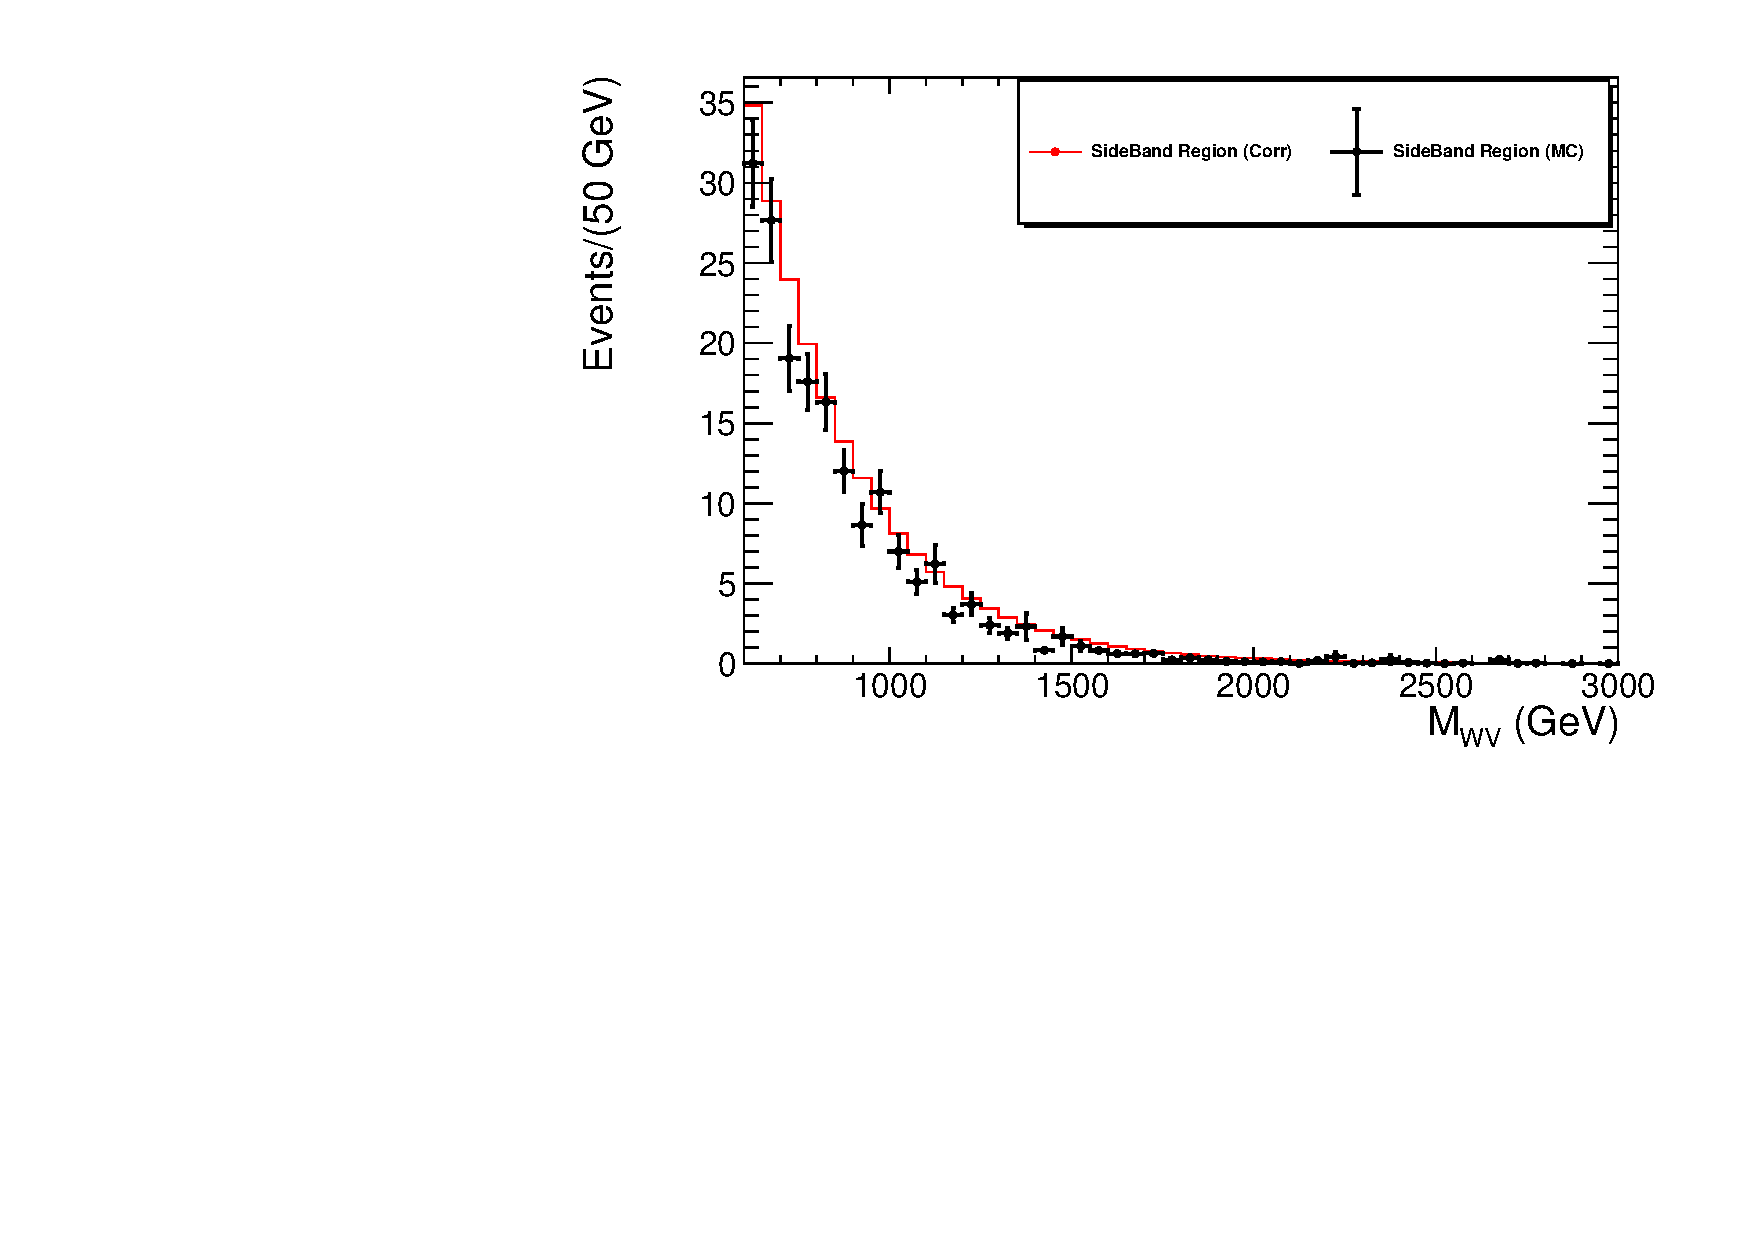
\includegraphics[width=0.48\textwidth]{Plots/BackgroundEstimation/WV/WVchannel_SideBandRegionComparison_VjetShape_MC_CorrShapeFromData.pdf}%
	 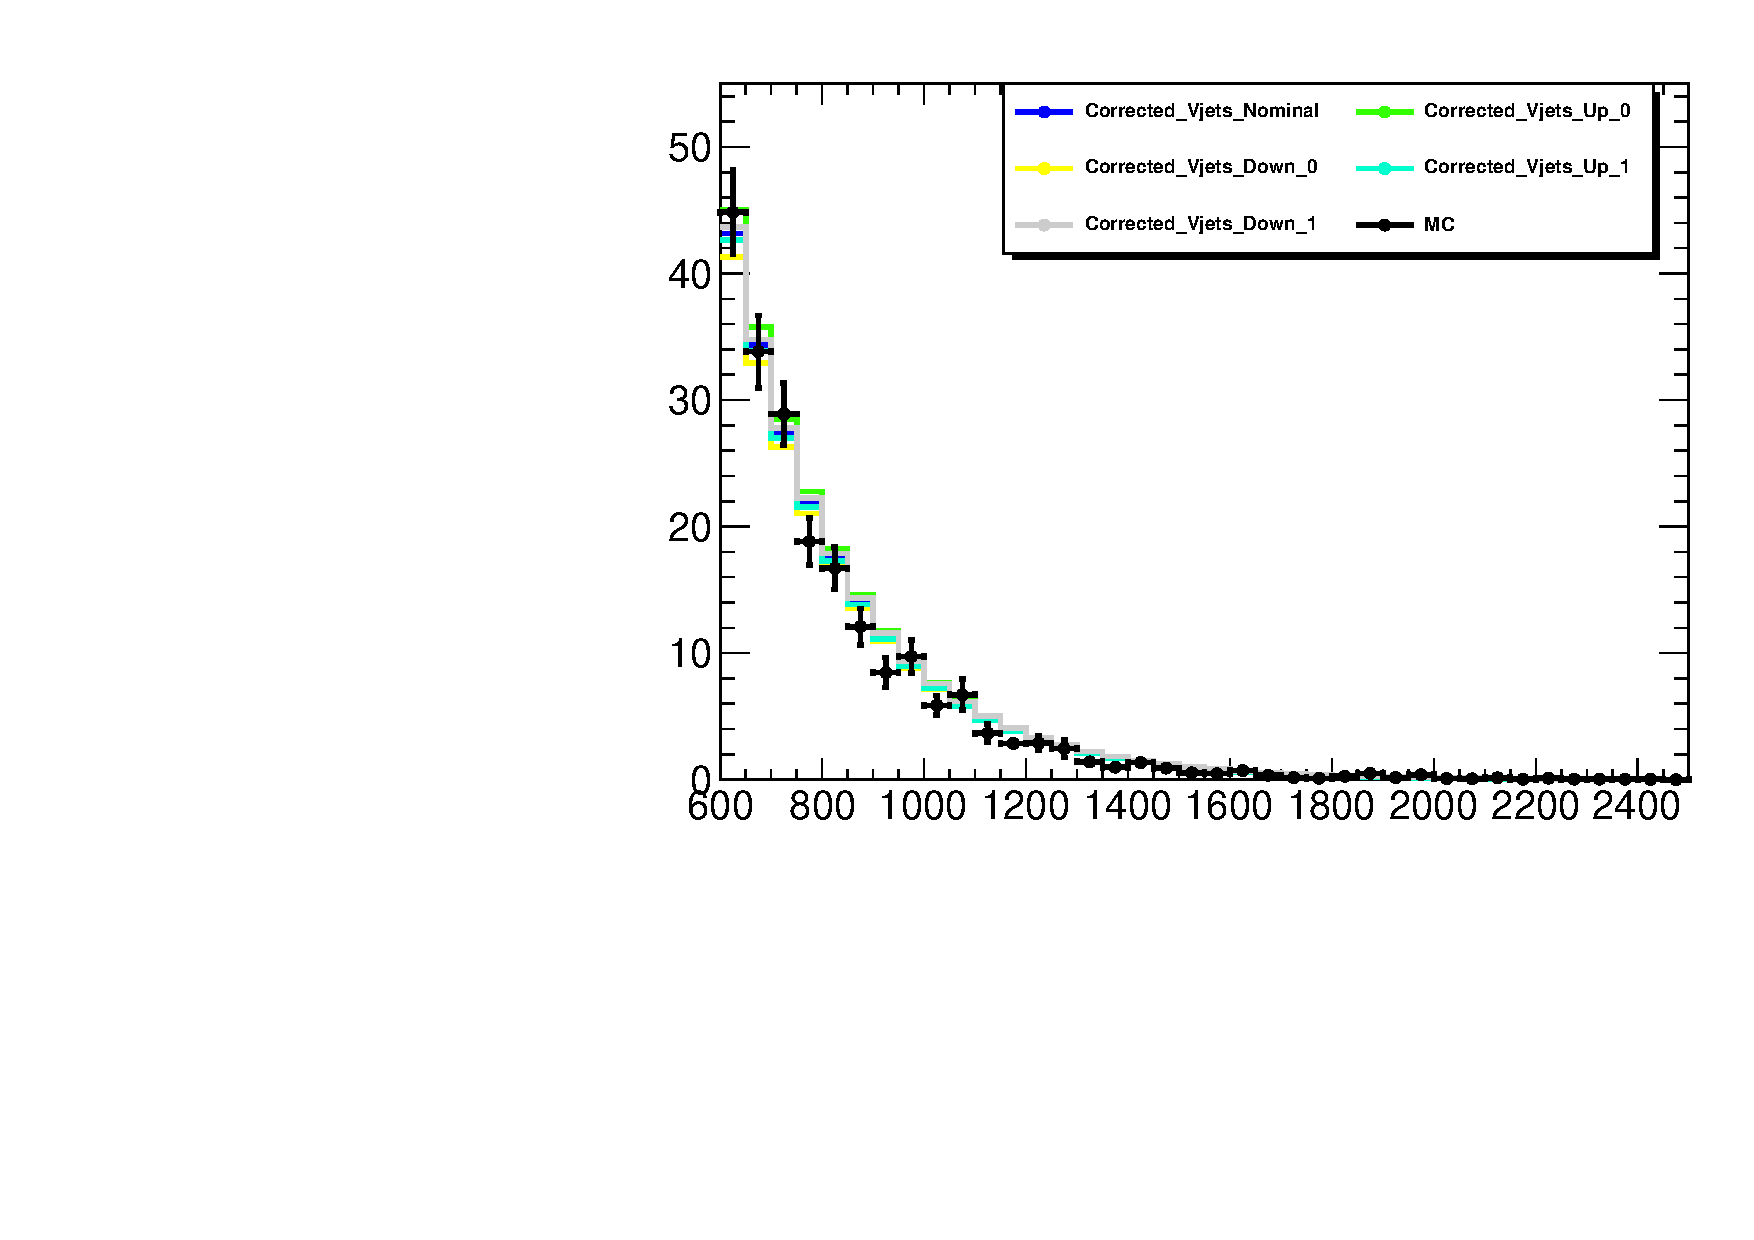
\includegraphics[width=0.48\textwidth]{Plots/BackgroundEstimation/WV/WVchannel_SignalRegionComparison_VjetShape_MC_CorrShapeFromData_38bin.pdf}
	 \caption{Comparison of the $W+$jet predictions using simulation (red) and the data-driven estimation in the sideband (left) and signal regions (right). The uncertainty band shows the fit uncertainty.}
	 \label{fig:signal}
\end{figure}
% \begin{figure}[h!]\ContinuedFloat
% 	 \centering 
% 	 \subfigure[]{\includegraphics[width=0.48\textwidth]{Plots/BackgroundEstimation/Wjet_SignalRegion_Nom_up_Down.png}}
% 	 \caption{}
% 	 \label{fig:WjetSignalRegionComp}
% \end{figure}

%\begin{figure}[htbp] 
%	 \centering 
%	 \begin{tabular}{cc}
%	 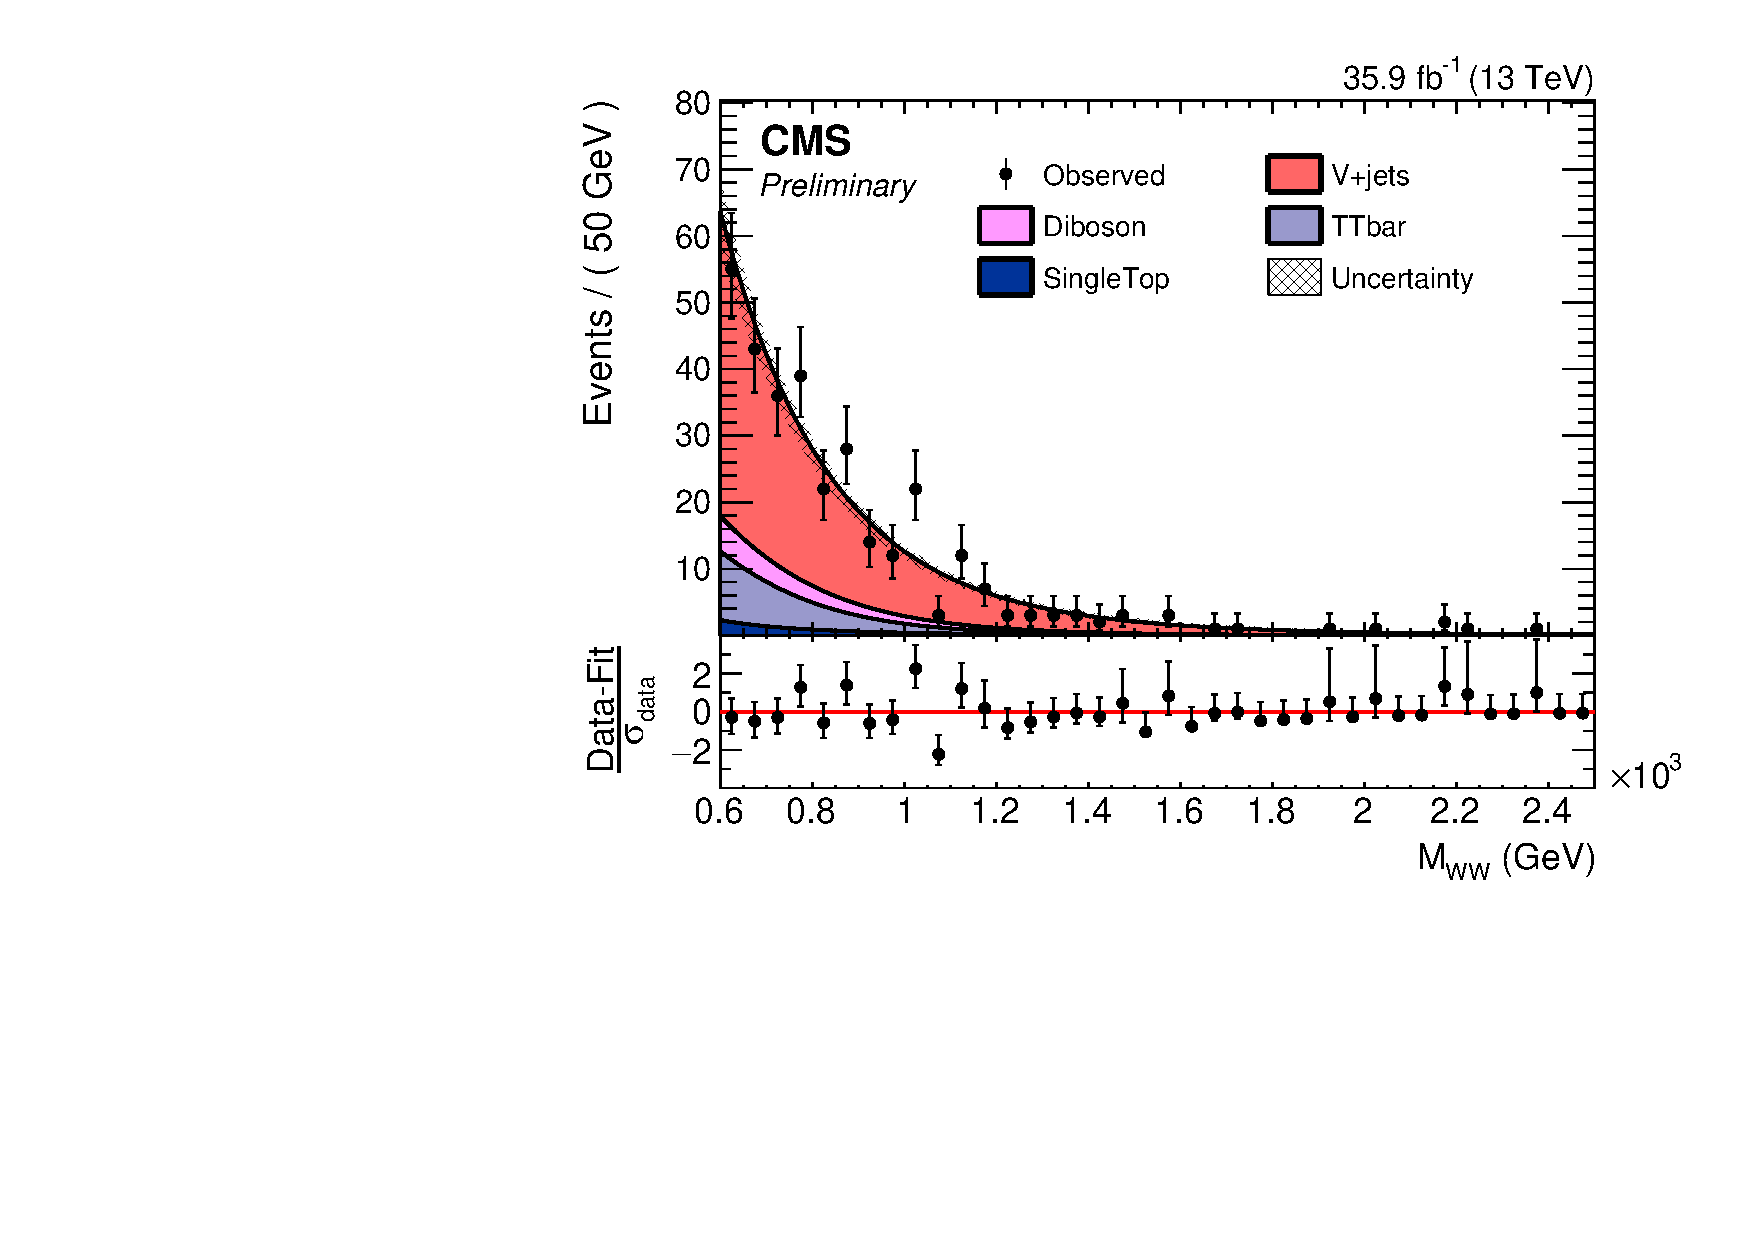
\includegraphics[width=0.48\textwidth]{Plots/BackgroundEstimation/WV/m_lvj_fitting/m_lvj_sb_lo_WJets0_xww__with_pull.pdf}
%	 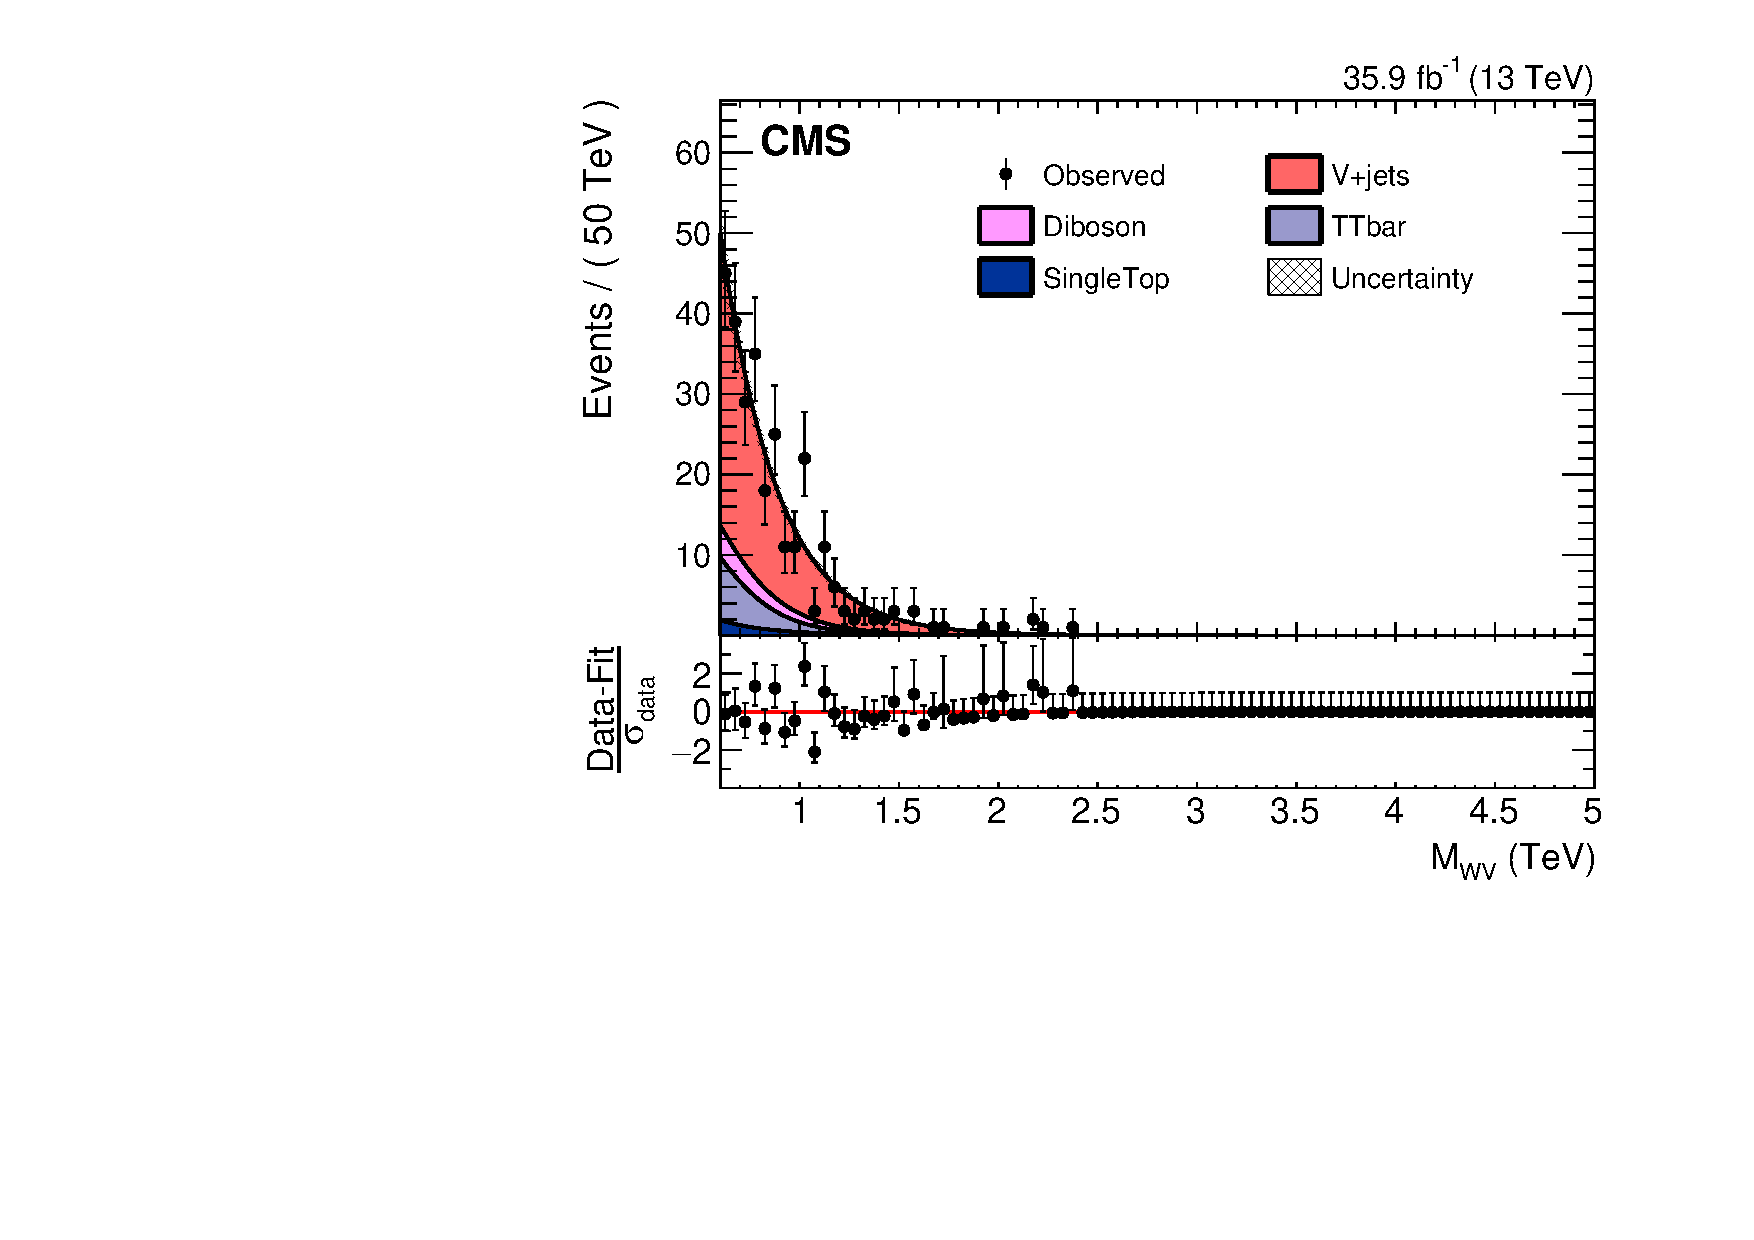
\includegraphics[width=0.48\textwidth]{Plots/BackgroundEstimation/WV/m_lvj_fitting/m_lvj_sb_lo_WJets01_xww__with_pull.pdf}\\
%	 \includegraphics[width=0.48\textwidth]{Plots/BackgroundEstimation/WV/DibosonBoostedElMuCuts13TeV_WjetControlRegion_Tighter_CHS_mass_lvj_type0_PuppiAK8_SBR.pdf}
%	 \includegraphics[width=0.48\textwidth]{Plots/BackgroundEstimation/WV/Cross_Check_DataMC_WithWjet_Corr.pdf}
%	 \end{tabular}
%	 \caption{Top: Both distribution are with corrected shape and normalization for W+Jets and other backgrounds shape are taken from fit function fitted to MC. Bottom (left): All backgrounds are taken from MC. Bottom (right): W+jet shape and normalization is taken after correction from data while all other backgrounds are taken from MC.}
%	 \label{fig:DataMCForMWW}
%\end{figure}

The statistical uncertainties from the fits in the sideband region are propagated to the final prediction. The statistical uncertainty in the alpha-ratio values due to limited number of simulated events are also propagated to the result. The $W+$jet prediction is also performed with an alternative function as shown above (Figure~\ref{fig:DataMCForMWW}) and the difference from the nominal prediction is taken as a systematic uncertainty.    

The normalization of the $W+$jet background in the sideband region is cross-checked by performing a fit to the $m_{V}$ distribution, excluding the signal region. The following parametric functions are used: 

\begin{description}
	\item [V+jets] $f_{User1} = \Big(1-\frac{x}{500}\Big)^p_0/\Big(\frac{x}{500}\Big)^p_1$ 
	\item [V+jets (alternative function)] $f_{ErfExp} = e^{(cx)}. \frac{1}{2}.\Big(1+Erf\big(\frac{x-offset}{width}\big)\Big)$
	\item [TTbar] $f_{2Gaus\_ErfExp} = f_1 \times \Big[e^{(cx)}. \frac{1}{2}.\Big(1+Erf\big(\frac{x-offset}{width}\big)\Big)\Big] + f_2 \times Gaus(x,\mu_1,\sigma_1) + f_3\times Gaus(x,\mu_2,\sigma_2) $
	\item [Single Top, Diboson] $f_{ExpGaus} = f_1 \times e^{(cx)} + Gaus(x,\mu,\sigma) $
\end{description}

The resulting shapes are shown in Figure~\ref{fig:mW_1}. The shown error band is determined by evaluating the fitted functions many times for several points along the x axis with the fitted parameters randomized according to their resulting uncertainty. The extracted fit parameters are summarized in Table~\ref{Table:BackgroundEst_fitPars}. These templates are then used to fit the $m_{V}$ distribution, excluding the signal region. The normalization and shape of the  $W$+jets process is floated in the fit. The other background processes are fixed to the SM predictions. The resulting fit is shown in Figure~\ref{fig:Wjet_SR_SBR_Comp}. The resulting normalization of the $W+$jet distribution agrees with the normalization obtained from the $m_{WV}$ fit.

% 1) 0xfc21990 RooRealVar::
\begin{table}[h!]
	\centering
	\begin{tabular}{||c | c||} 
	 \hline
	  parameter & Values \\
	 \hline \hline
	 \multicolumn{2}{|c|}{W+jets ($f_{User1}$)}\\
	 \hline
	 $p_0$		&	25.0479 $\pm$ 0.885452\\
	 $p_1$		&	-4.03783 $\pm$ 0.328605\\
	 $N$		&	478.191 $\pm$ 35.4216\\
	 \hline \hline
	 \multicolumn{2}{|c|}{W+jets (alternate function, $f_{ErfExp}$)}\\
	 \hline
	 c 			&	-0.0228734 $\pm$ 0.00217427\\
	 offset 	&	50.9183 $\pm$ 2.56036\\
	 width 		&	13.7415 $\pm$ 3.89626\\
	 $N$		&	460.073 $\pm$ 34.2282\\
	 \hline \hline
	 \multicolumn{2}{|c|}{Diboson, $f_{ExpGaus}$}\\
	 \hline 
	 $f_1$		&	0.452621 $\pm$ 0.0175585\\
	 c 			&	-0.00625601 $\pm$ 0.00115951 \\
	 $\mu$		&	82.3131 $\pm$ 0.39325\\
	 $\sigma$	&	10 $\pm$ 9.41247e-07\\
	 $N$		&	87.2154 $\pm$ 1.89749\\
	 \hline \hline
	 \multicolumn{2}{|c|}{TTbar, $f_{2Gaus\_ErfExp}$}\\
	 \hline 
	 $f_1$		&	0.320894 $\pm$ 0.0891809\\
	 c 			&	-0.0254783 $\pm$ 0.00692614\\
	 offset 	&	79.35 (constant)\\
	 width 		&	30.1227 $\pm$ 5.73131\\
	 $f_2$		&	0.67125 (constant)\\
	 $\mu_1$	&	82.7893 $\pm$ 0.609335\\
	 $\sigma_1$	&	8.51989 $\pm$ 0.780058\\
	 $f_3$		&	1.0 (constant)\\
	 $\mu_2$	&	$\mu_1$ + 6.9129 \\
	 $\sigma_2$	&	$\sigma_1$ + 3.6819\\
	 $N$		&	152.598 $\pm$ 4.8036\\
	 \hline \hline
	 \multicolumn{2}{|c|}{Single-Top, $f_{ExpGaus}$}\\
	 \hline 
	 $f_1$		&	0.471434 $\pm$ 0.080531\\
	 c 			&	-0.00367233 $\pm$ 0.00476394 \\
	 $\mu$		&	82.6023 $\pm$ 1.16547\\
	 $\sigma$	&	8.25865 $\pm$ 1.01946\\
	 $N$		&	35.5749 $\pm$ 2.98679\\
	 \hline 
	\end{tabular}
 	\caption{Extracted fit parameters for the functions describing the $m_{V}$ distributions.}
 	\label{Table:BackgroundEst_fitPars}
\end{table}


\begin{figure}[htbp] 
	 \centering 
	 \begin{tabular}{cc}
	 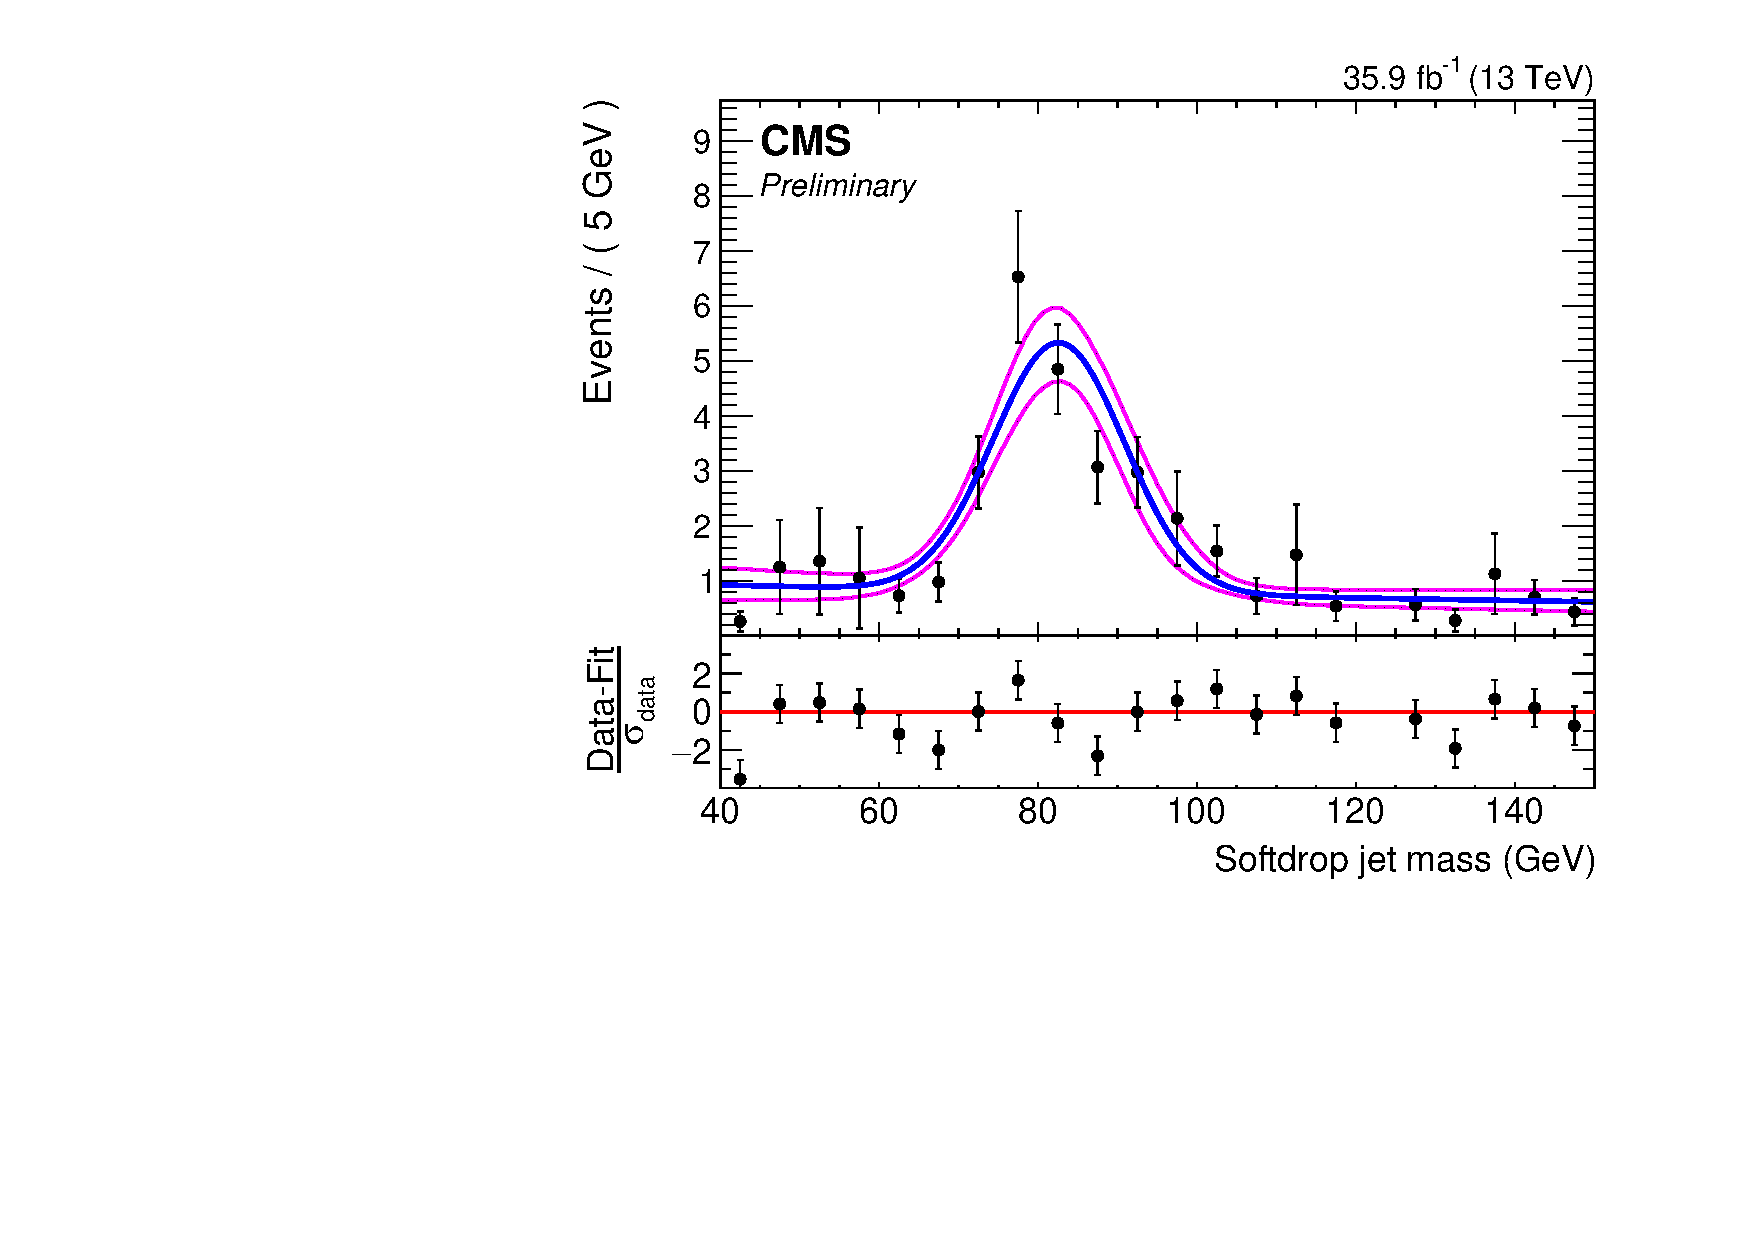
\includegraphics[width=0.45\textwidth]{Plots/BackgroundEstimation/WV/m_j_fitting/_STop_xwwWWTree_STop_ExpGaus_with_pull.pdf}
	 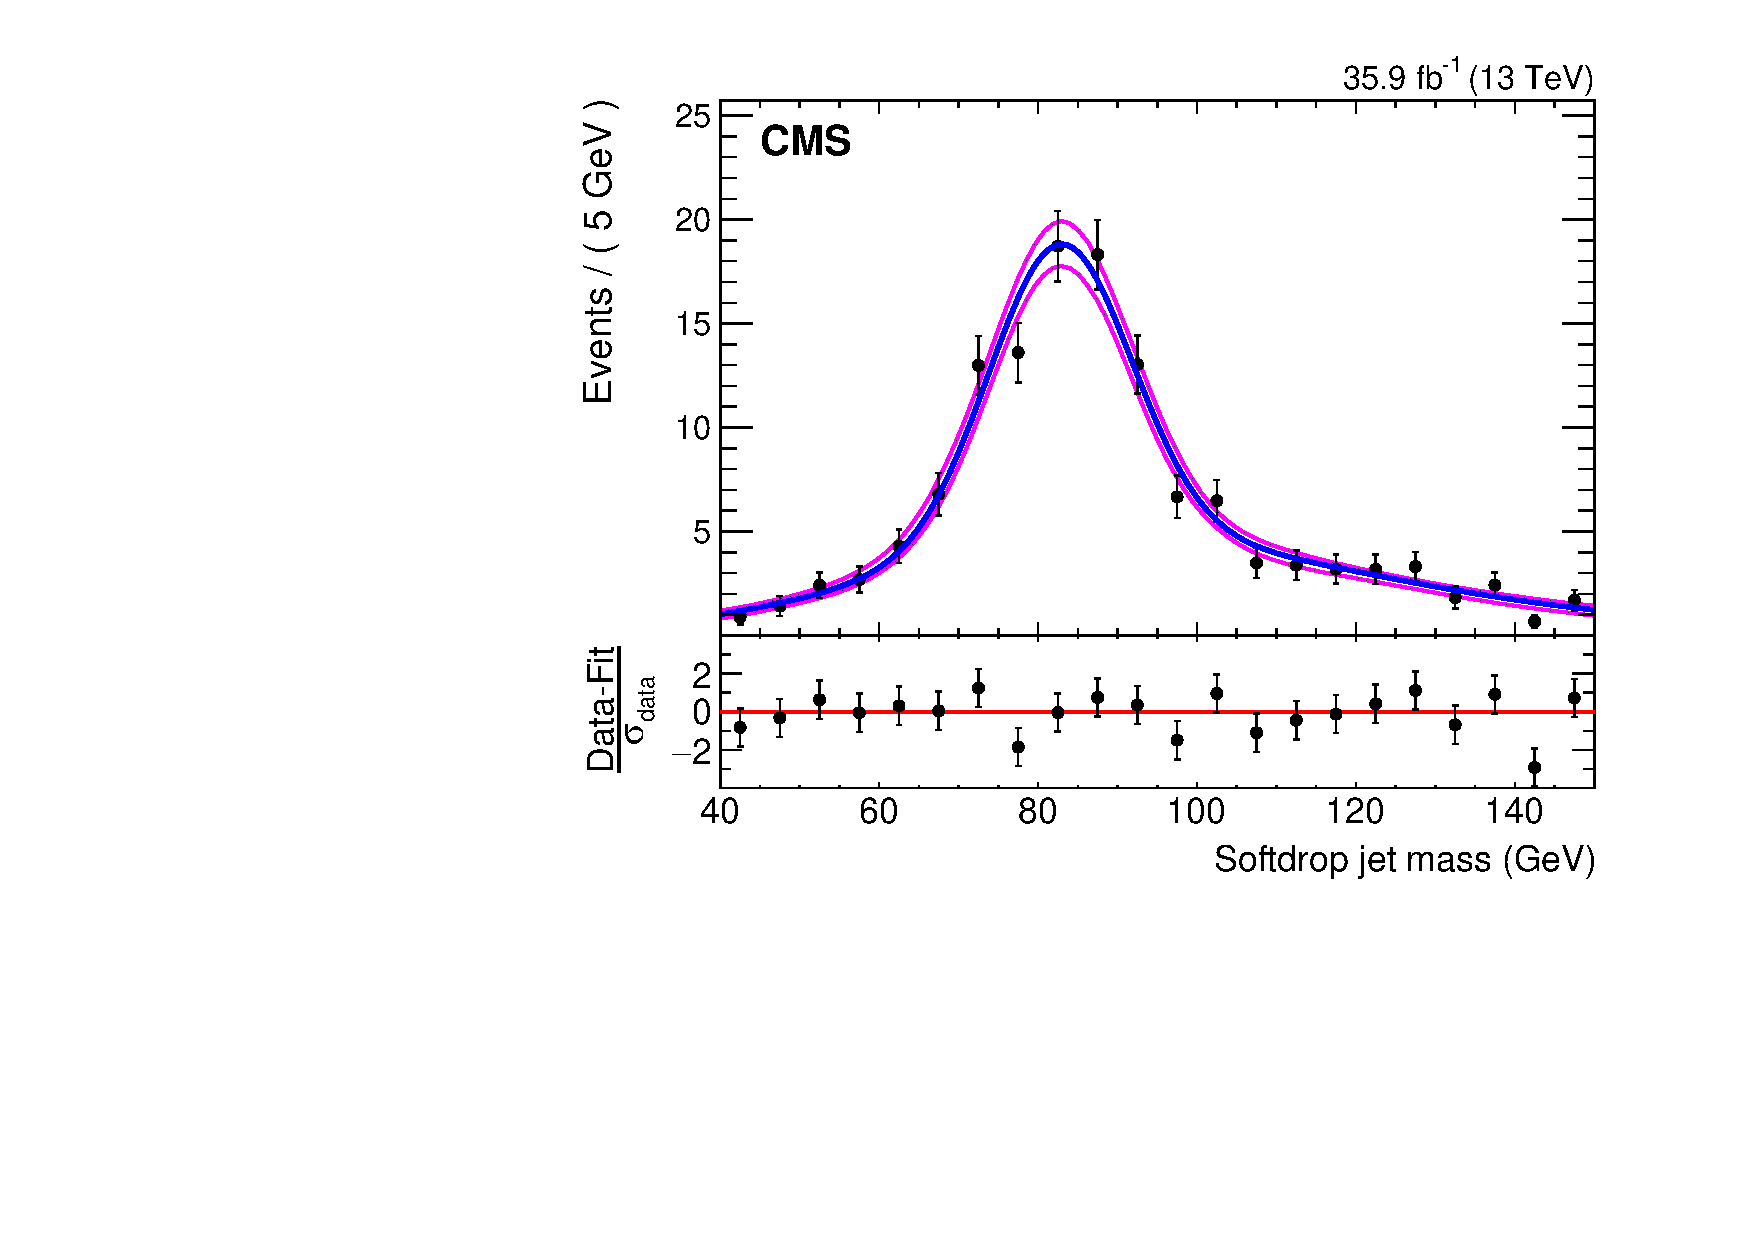
\includegraphics[width=0.45\textwidth]{Plots/BackgroundEstimation/WV/m_j_fitting/_TTbar_xwwWWTree_TTbar_2Gaus_ErfExp_with_pull.pdf}\\
	 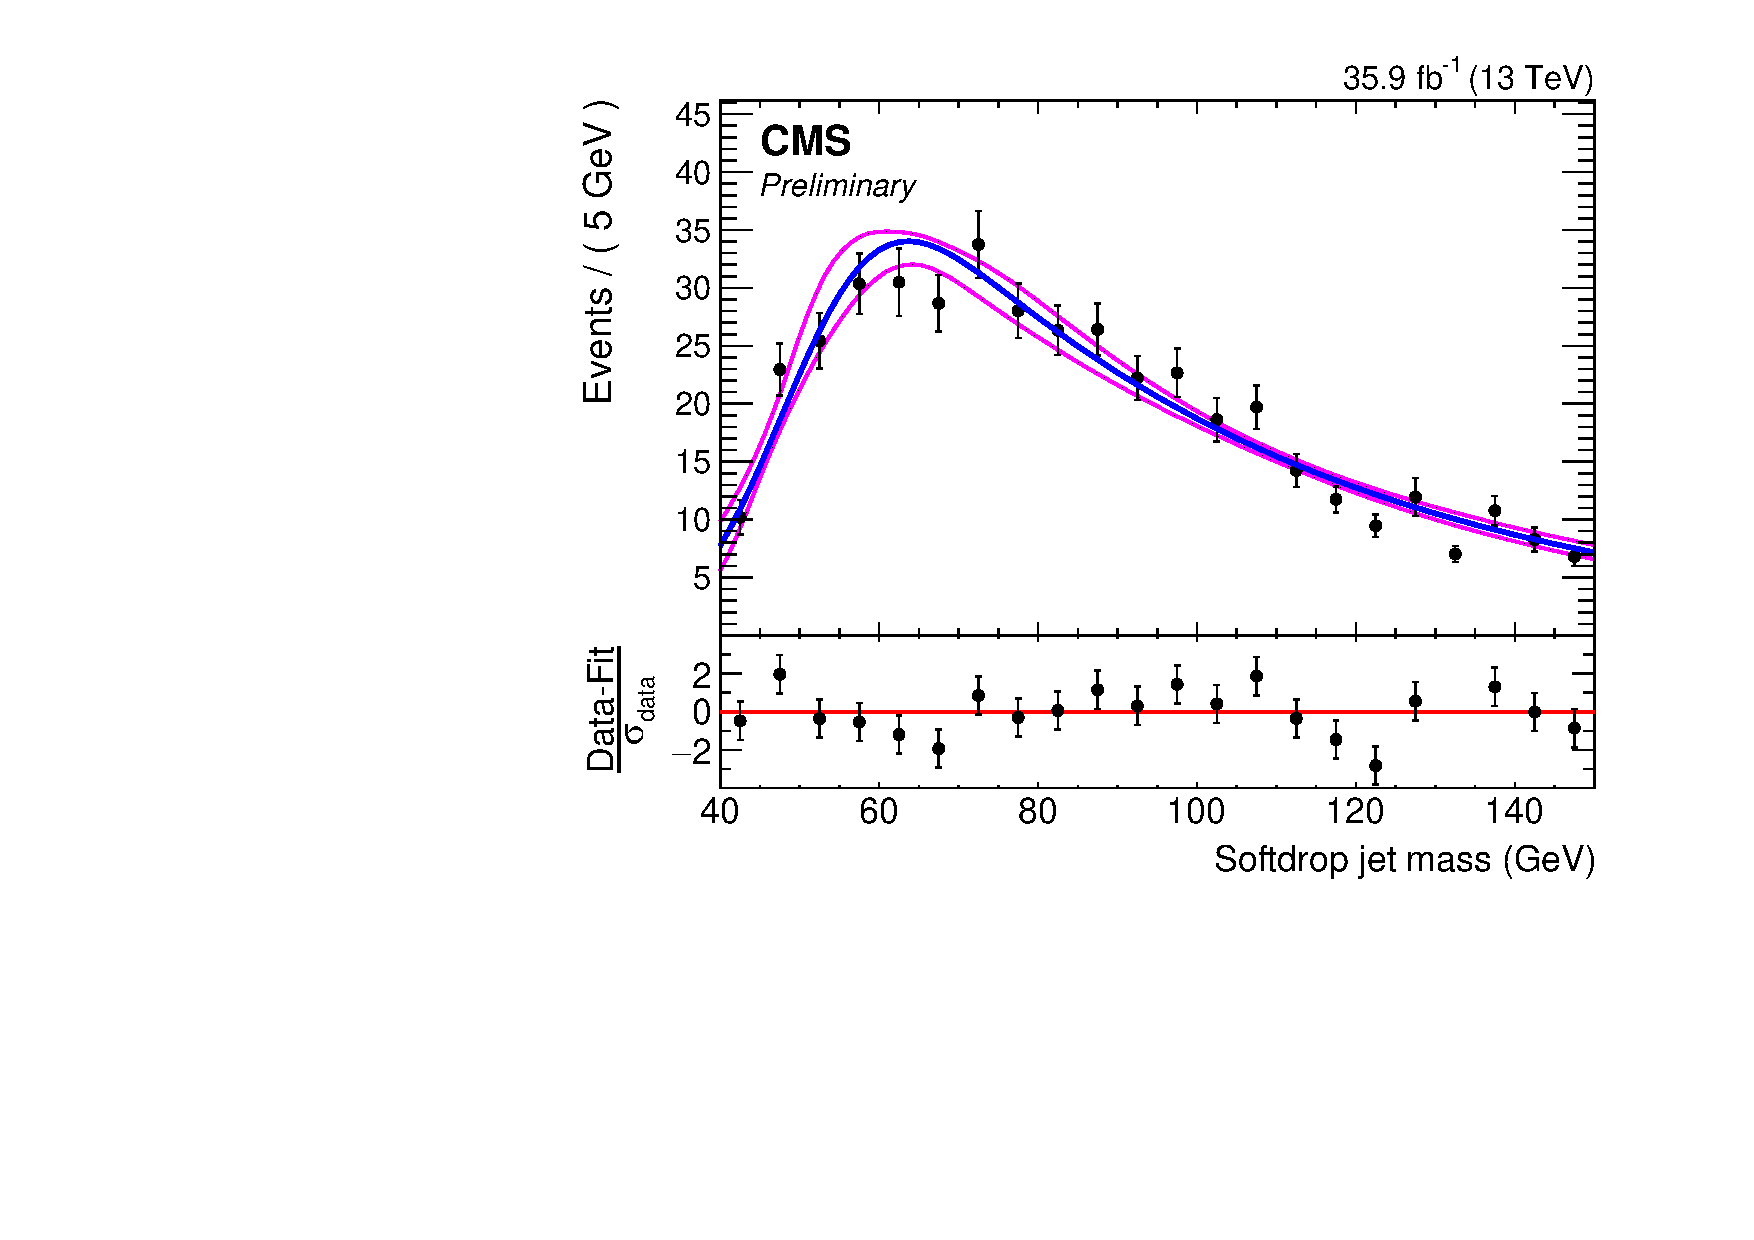
\includegraphics[width=0.45\textwidth]{Plots/BackgroundEstimation/WV/m_j_fitting/_WJets01_xwwWWTree_VJets_ErfExp_with_pull.pdf}
	 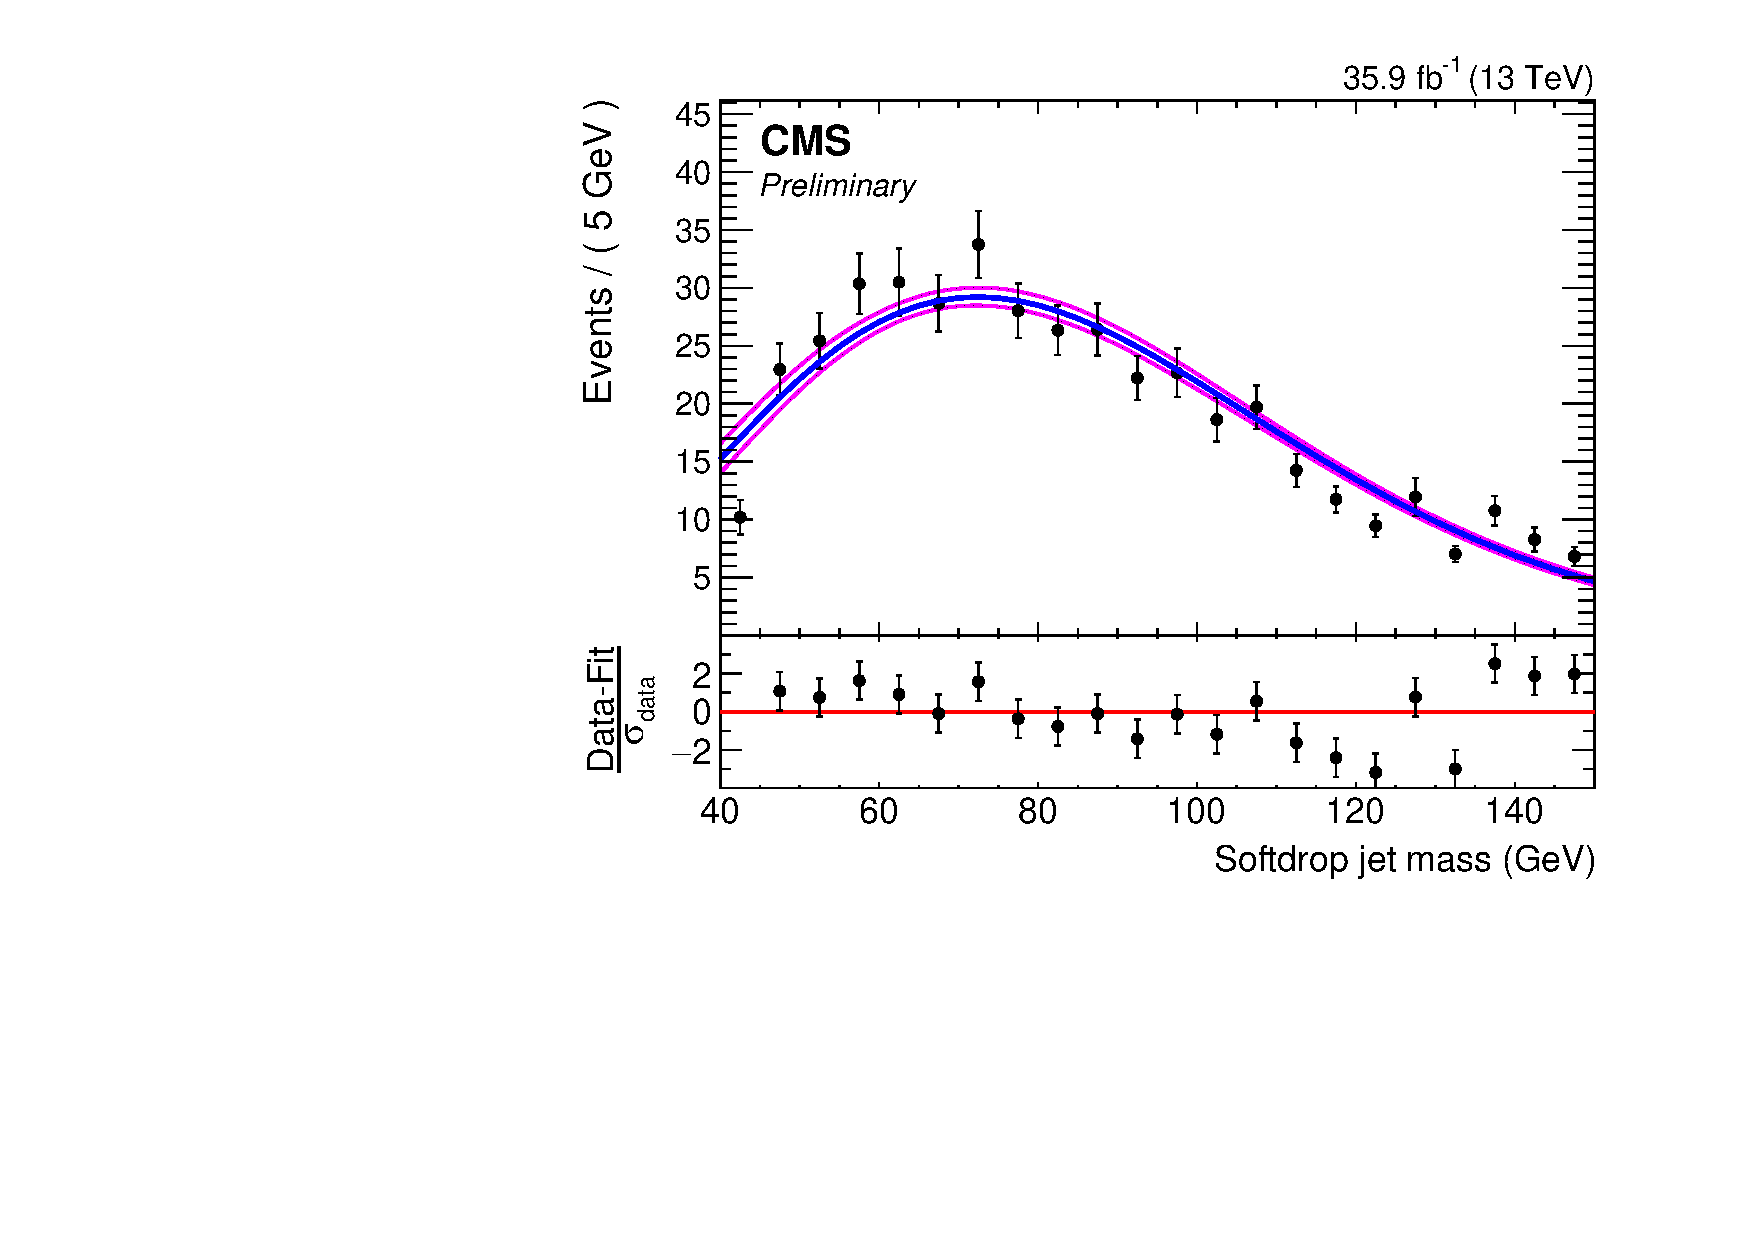
\includegraphics[width=0.45\textwidth]{Plots/BackgroundEstimation/WV/m_j_fitting/_WJets0_xwwWWTree_VJets_User1_with_pull.pdf}\\
	 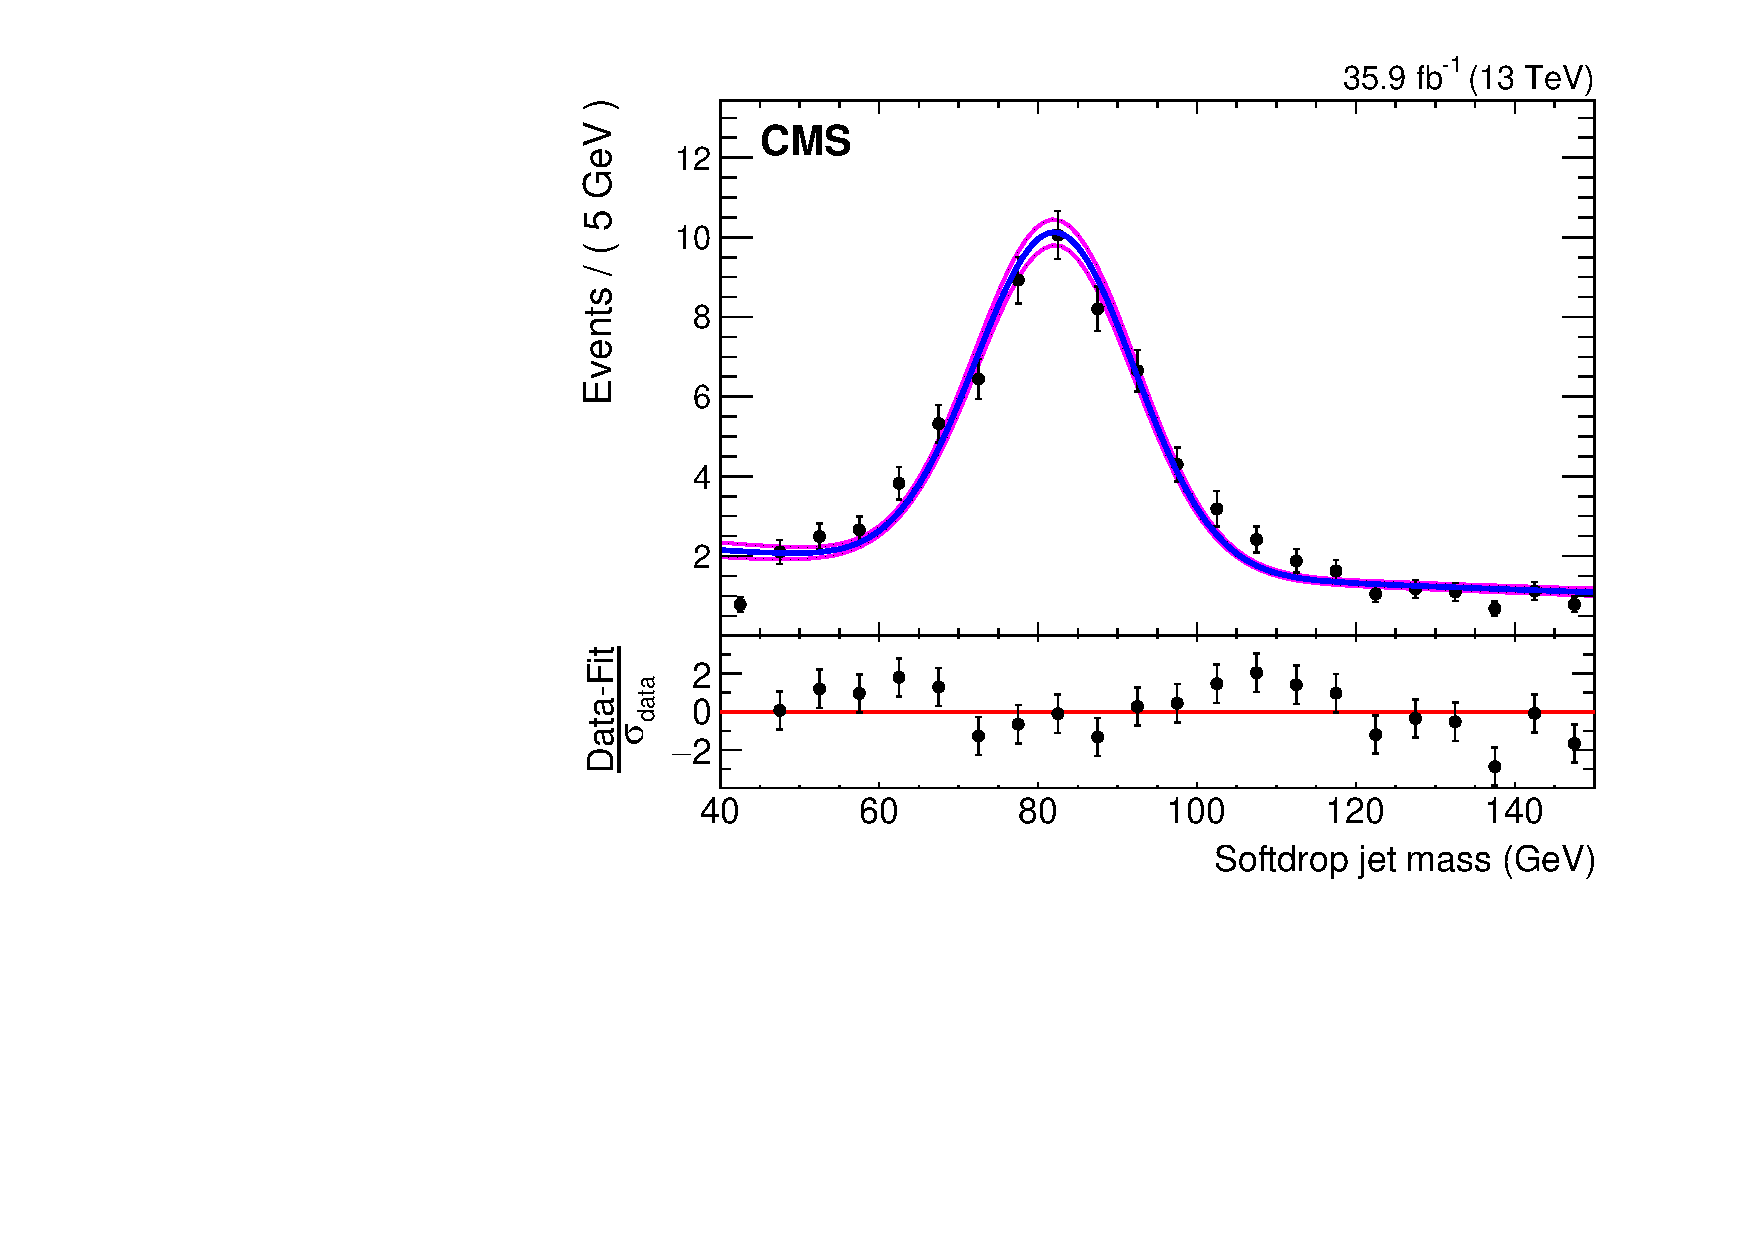
\includegraphics[width=0.45\textwidth]{Plots/BackgroundEstimation/WV/m_j_fitting/_VV_xwwWWTree_VV_EWK_QCD_ExpGaus_with_pull.pdf}
	 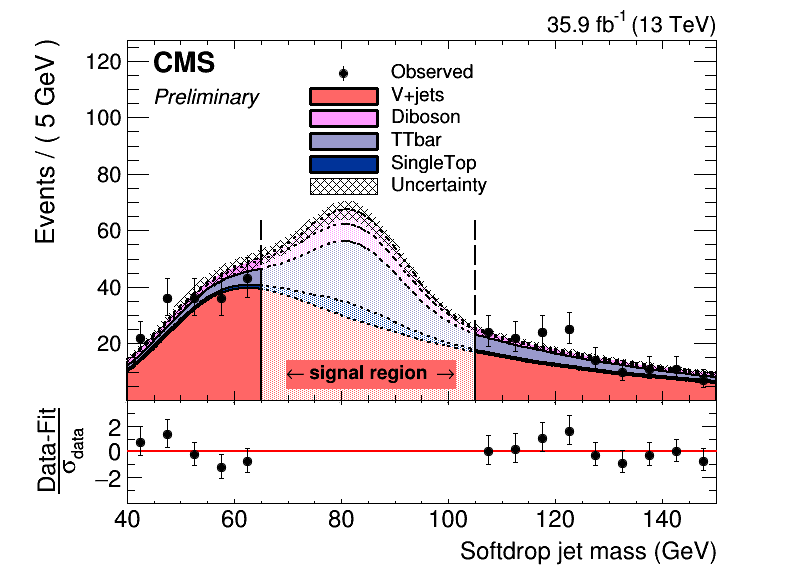
\includegraphics[width=0.45\textwidth]{Plots/BackgroundEstimation/WV/m_j_fitting/m_j_sideband_WJets01_xww__with_pull.png}\\
	 \end{tabular}
	 \caption{MC fit distribution for $m_{V}$. Top Left: Single top, Top right: TTbar, Middle left: Wjets with $f_{ErfExp}$, Middle right: Wjets with $f_{User1}$, Bottom: Diboson distribution }
	 \label{fig:mW_1}
\end{figure}


\begin{figure}[htbp] 
	 \centering 
	 \begin{tabular}{cc}
	 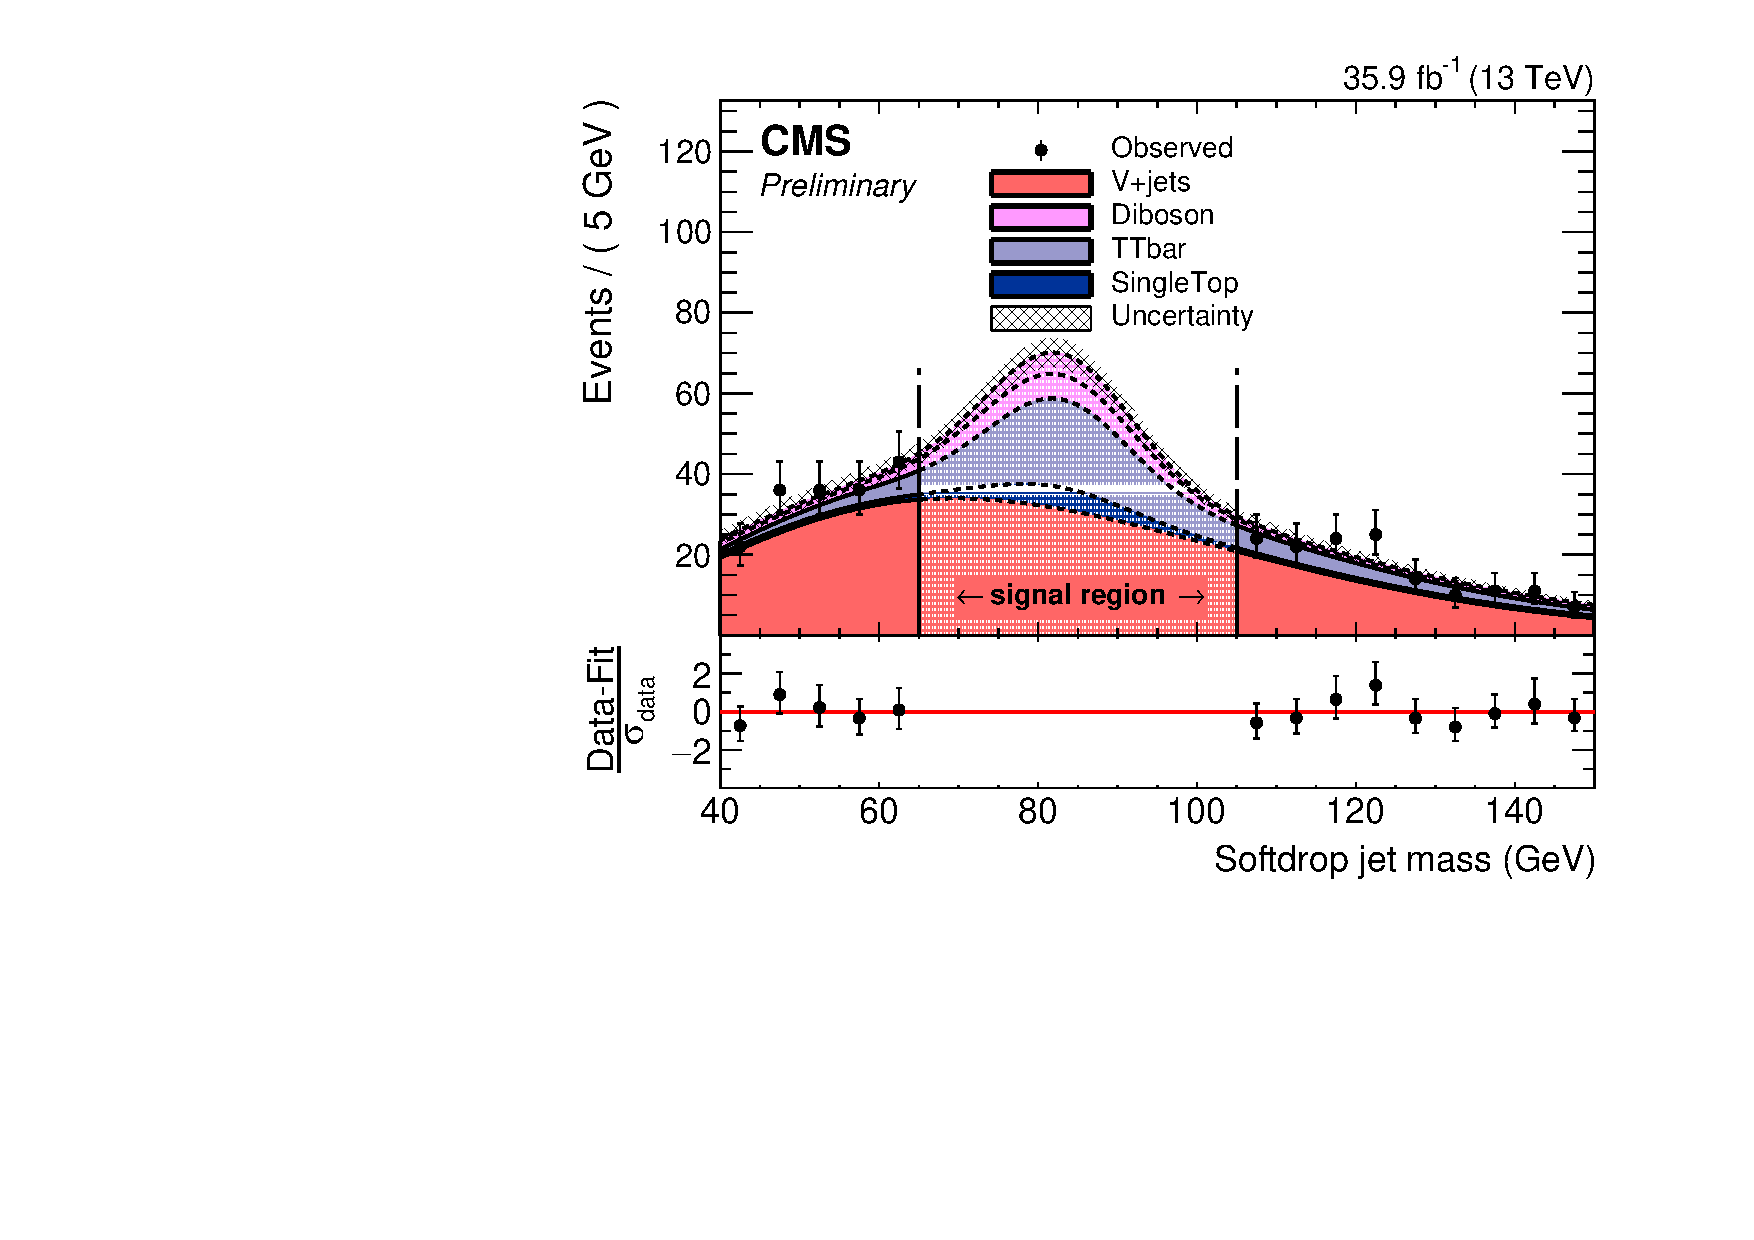
\includegraphics[width=0.48\textwidth]{Plots/BackgroundEstimation/WV/m_j_fitting/m_j_sideband_WJets0_xww__with_pull.pdf}
	 \end{tabular}
	 \caption{Result of the normalization fit in the $m_{V}$ spectrum.}
	 \label{fig:Wjet_SR_SBR_Comp}
\end{figure}


\subsection{Closure Test}
The closure of the background estimation method is checked. The contribution of the $W+jet$ process is estimated in $105~GeV<~m_{WV}<125~GeV$ sideband region by repeating the background estimation above using a reduced sideband region given by requiring $40~GeV < m_{V} < 65~GeV$ or $125~GeV < m_{V} < 150~GeV$. Figure~\ref{fig:closure} shows (left) that the prediction of the background processes in $105~GeV<~m_{WV}<125~GeV$ sideband region is in good agreement with the data. For comparison, the predictions taken from simulation are also shown (right). 

\begin{figure}[htbp] 
	 \centering 
	 \begin{tabular}{cc}
	 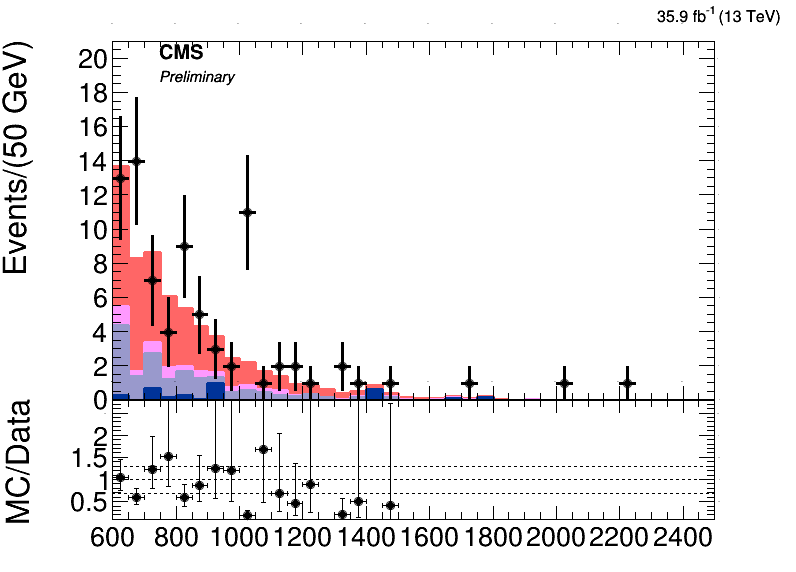
\includegraphics[width=0.48\textwidth]{Plots/BackgroundEstimation/WV/signal_region_Closure_test_AfterCorrShape_38bins.png}
         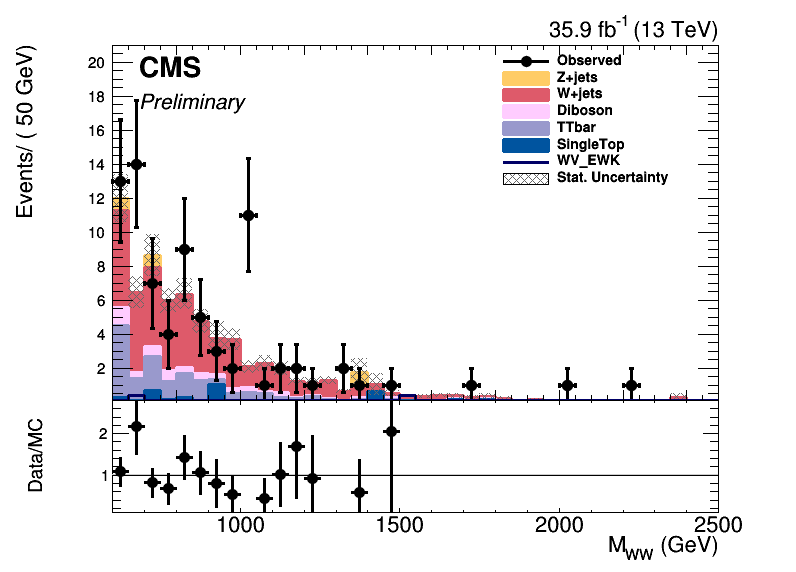
\includegraphics[width=0.48\textwidth]{Plots/BackgroundEstimation/WV/DibosonBoostedElMuCuts13TeV_WjetControlRegion_Tighter_CHS_mass_lvj_type0_PuppiAK8_ClosureTest_SignalRegion.png}  
	 \end{tabular}
	 \caption{The data and predicted $m_{WV}$ distribution obtained from the alpha-ratio method (left) and simulation (right).}
	 \label{fig:closure}
\end{figure}


\section{$Z+$jets}
The $Z+$jet background process prediction in the $Z V$ final state is performed using the alpha-ratio method descriped above. The methods to obtain the prediction and the corresponding systematic uncertainties are identical to what was done for the $W+$jet prediction in the $W V$ final state. Figure~\ref{fig:zvfits} shows the corresponding fit of the $m_{ZV}$ distribution in the sideband region in the $Z V$ final state.  

\begin{figure}[htbp] 
	 \centering 
	 \begin{tabular}{cc}
	 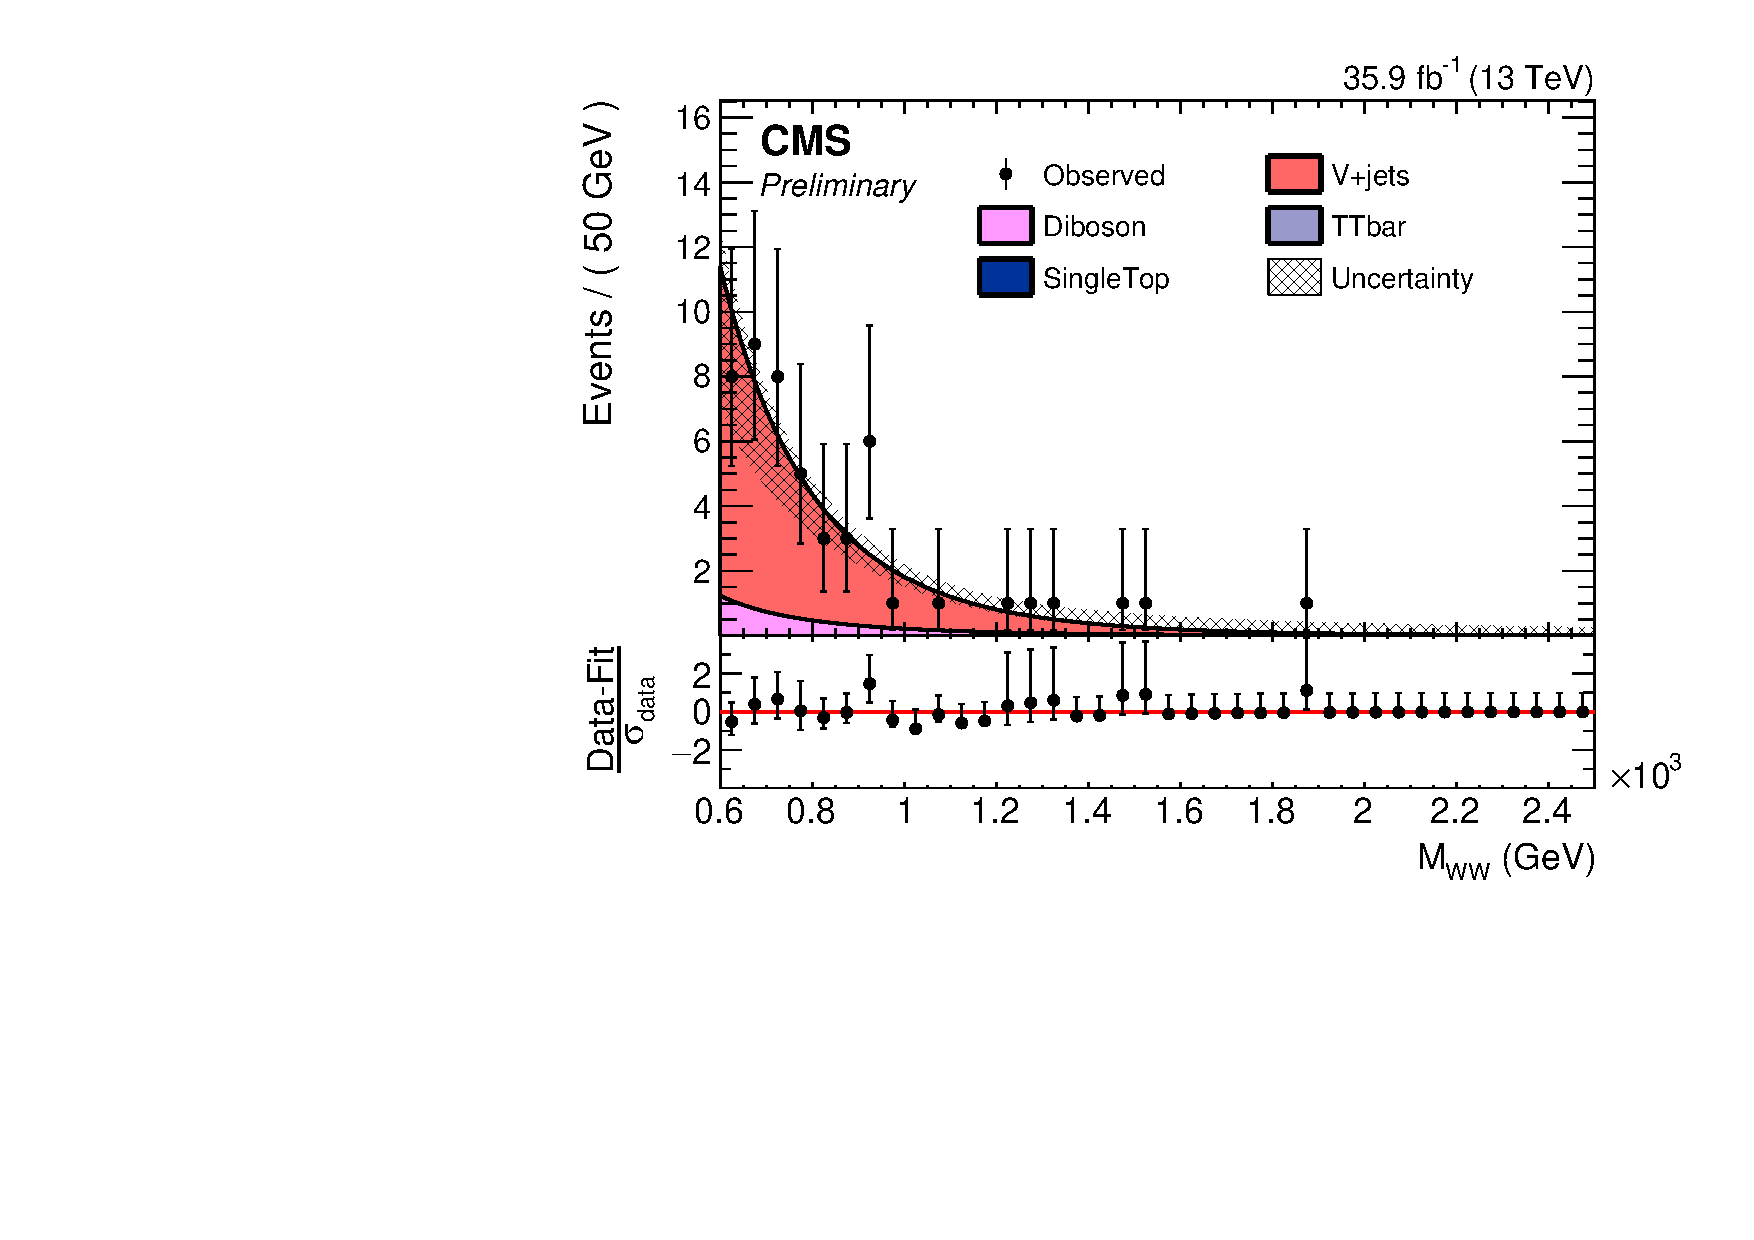
\includegraphics[width=0.48\textwidth]{Plots/BackgroundEstimation/ZV/m_lvj_fitting/m_lvj_sb_lo_WJets0_xww__with_pull.pdf}
	 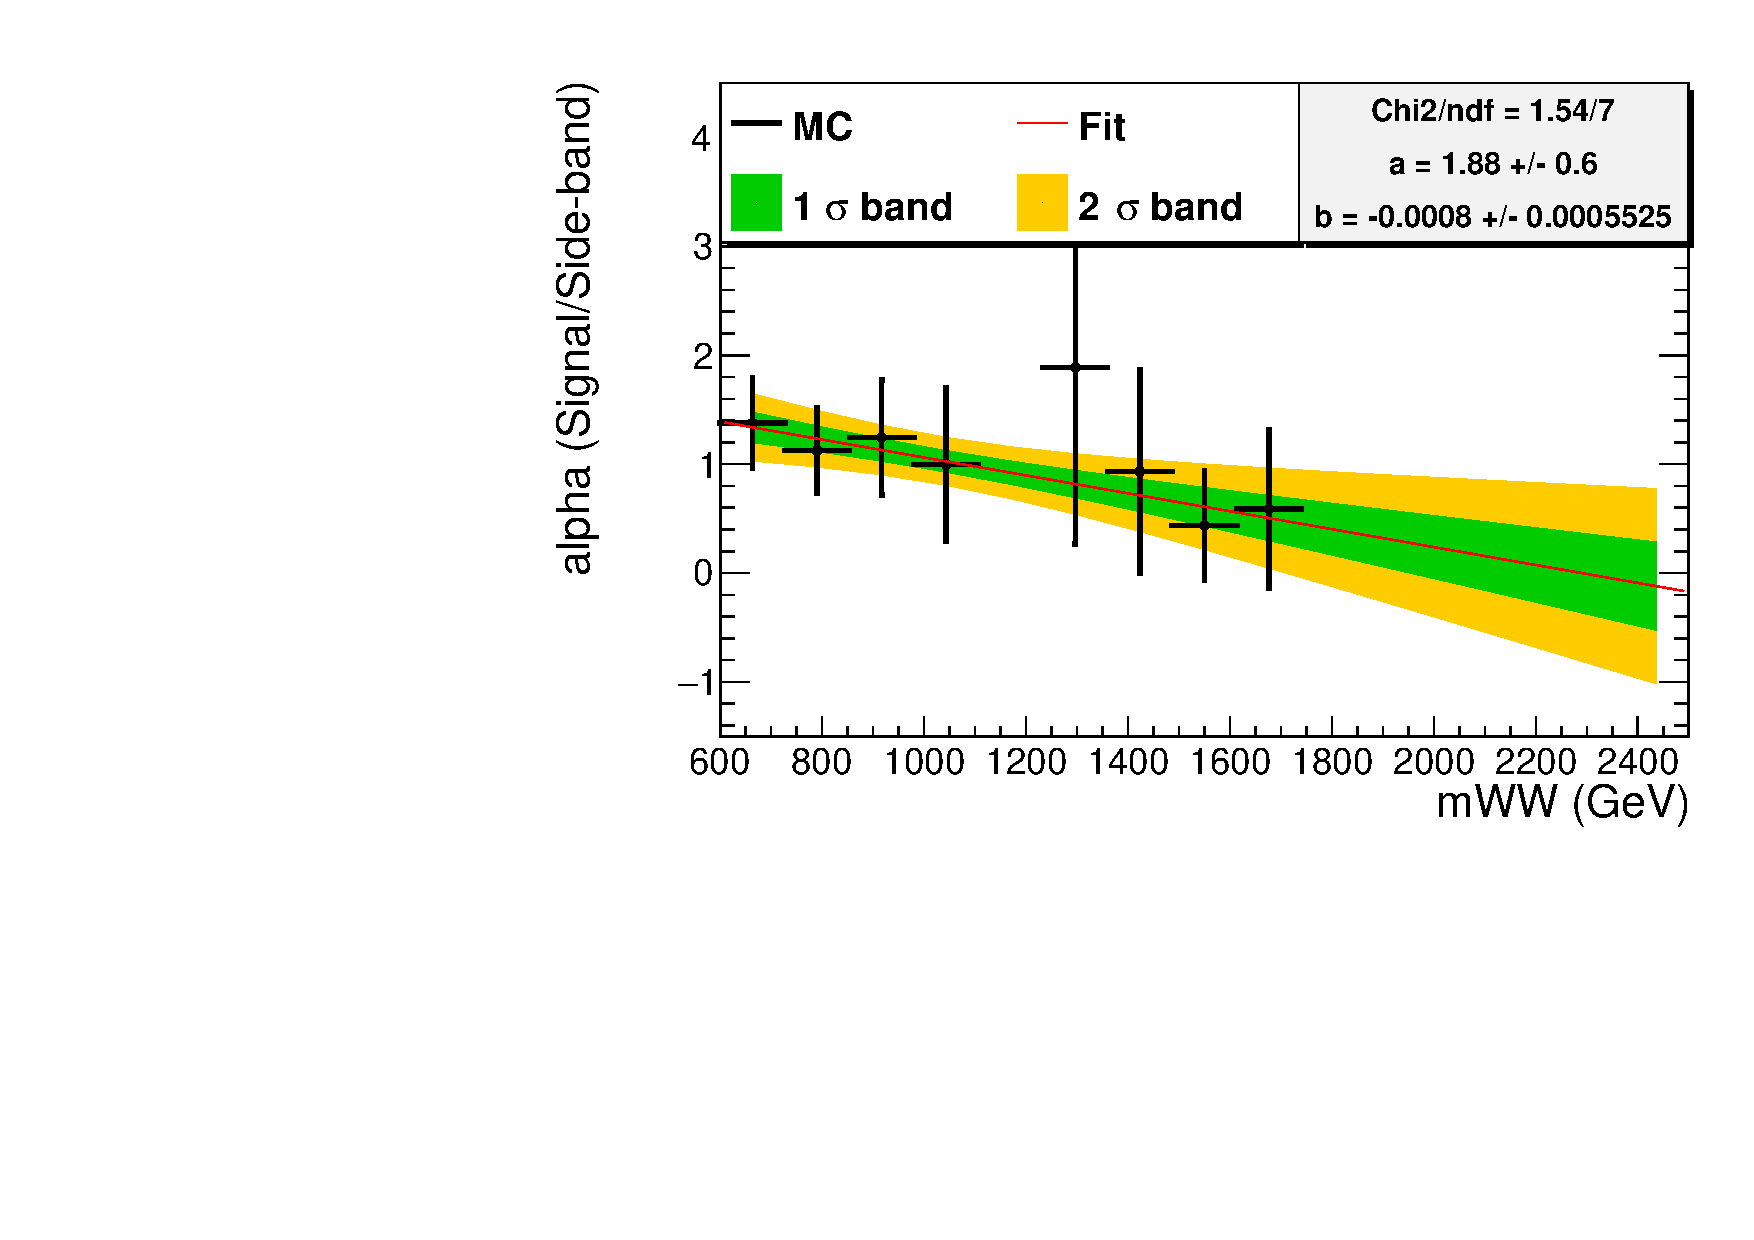
\includegraphics[width=0.48\textwidth]{Plots/BackgroundEstimation/ZV/ZVchannel_AlphaDistribution_AfterFit.pdf}
	 \end{tabular}
	 \caption{The data distribution and the corresponding fit of the $m_{ZV}$ distribution in the sideband region (left).Alpha-ratio value distribution (right).}
	 \label{fig:zvfits}
\end{figure}
% % chapter background_estimation (end)